\documentclass[a4paper,12pt]{report}
\usepackage{a4wide}

%\documentclass[a5paper,10pt]{book}
%\usepackage[top=23mm, bottom=18mm, left=15mm, right=25mm]{geometry}
%\geometry{papersize={170mm,220mm}}


\usepackage[utf8x]{inputenc}
\usepackage[danish]{babel}

\usepackage{xr-hyper} %Externe hyper-ref
\usepackage[colorlinks=true, hyperindex=true, linkcolor=minmblaa, citecolor=minmblaa, urlcolor=minmblaa]{hyperref}
\hypersetup{colorlinks=true,filecolor=minmblaa,bookmarksnumbered=true} %Til hyperreferencer. Referencer med farver
\usepackage{needspace} % giver mulighed for at kræve at der skal være et antal tomme linier på siden før ellers indsættes et sideskift.
\usepackage{framed} %Bokse
\usepackage{wrapfig}

\usepackage{amsmath,amsfonts,amssymb,amsthm,mathtools} %Matematikpakker

\setlength{\parindent}{0mm} %Ingen Indhak i første linje i afsnit

\usepackage{color} %Farvepakke

\usepackage{array}
\usepackage{colortbl}
\usepackage{multirow} %Til at flette rækker i tabeller.

\usepackage{verbatim,mhchem}



	% DOWNLOAD FRA: http://sarovar.org/frs/?group_id=52&release_id=97
	% Læg i directory for hoved TEX fil
%\usepackage[draft]{pdfdraftcopy}
%\draftstring{Licens: Kasper Langt Mellemnavn Skårhøj}
%\draftfontsize{30}
	%\draftfontfamily{hlh}
	%\draftangle{45}
	%\definecolor{mycolor}{rgb}{.825,.855,1}
	%\draftcolor{mycolor}
	%\draftfontattrib



% = Sidehoved =
\usepackage{fancyhdr}
\pagestyle{fancy}
\renewcommand{\sectionmark}[1]{\markright{\protect\titlegraphic{dturoed}\textcolor{dtugraa}{\thesection~\MakeUppercase{#1}}}} % \thesection.\
\fancyhead{}
\fancyfoot{}
\fancyhead[R]{\titlefont\thepage}
\fancyhead[C]{}
\fancyhead[L]{\titlefont \small eNote \MakeUppercase{~\thechapter}~\hspace*{1ex}\rightmark}
\renewcommand\headrulewidth{0pt}
\fancypagestyle{plain}{\fancyfoot[C]{}}% {\titlefont\footnotesize\thepage}}
\setlength{\headheight}{15pt}


% = Længder
%\newlength{\envtblsep}\setlength{\envtblsep}{1\FrameSep}
\newlength{\obsl}\setlength{\obsl}{\textwidth-1.2cm-13.2pt}

% Includes:

% =     Fonts (select one)    =
\usepackage{mathpazo}\linespread{1.05} % Palatino needs more leading (space between lines)
\usepackage{bm} % bold math, must be loaded after the fontpackages

% % Til overskrifter
\DeclareTextFontCommand{\th}{\fontencoding{T1}\fontfamily{phv}\fontseries{b}\selectfont}
\newcommand\titlefont{\fontencoding{T1}\fontfamily{phv}\selectfont}


% =     PGF grafik      =
\usepackage{tikz}
\newcommand\titlegraphic[1]{%
\tikz[baseline] %
\draw[thick,color=#1]
(0pt  ,-0.25em) -- (0pt  ,0.85em)
(2.5pt,-0.25em) -- (2.5pt,0.85em)
(5pt  ,-0.25em) -- (5pt  ,0.85em)
(7.5pt,-0.25em) -- (7.5pt,0.85em);\hspace*{0.8ex} %
}

\newcommand\titlegraphicwide[1]{%
\tikz[baseline] %
\draw[line width=0.8mm,color=#1]
(0pt  ,-0.25em) -- (0pt  ,0.85em)
(4.5pt,-0.25em) -- (4.5pt,0.85em)
(9pt  ,-0.25em) -- (9pt  ,0.85em)
(13.5pt,-0.25em) -- (13.5pt,0.85em);\hspace*{0.8ex} %
}


% =      Title Layout      =
\usepackage{titlesec}
\makeatletter
\titleformat{\chapter}
	[display] % Shape
	{\titlefont\Huge\flushleft} % Title and label format
	{\titlefont\LARGE\bfseries \titlegraphicwide{dturoed}\textcolor{dtugraa}{\@chapapp~\thechapter}} % label
	{0.9em} % label/title separation
	{} % before code
	[] % after code
\makeatother
\titleformat{\section}
	[hang] % Shape
	{\titlefont\Large\flushleft} % Title and label format
	{\thesection} % label
	{0.9em} % label/title separation
	{} % before code
	[] % after code
\titleformat{\subsection}
	[hang] % Shape
	{\titlefont\large} % Title and label format
	{\thesubsection} % label
	{0.9em} % label/title separation
	{} % before code
	[] % after code
\titlespacing{\subsection}{0pt}{*6}{*1.5}
\titleformat{\subsubsection}
	[hang] % Shape
	{\titlefont} % Title and label format
	{\thesubsubsection} % label
	{0.9em} % label/title separation
	{} % before code
	[] % after code



% = Farver
\definecolor{dturoed}{rgb}{0.6, 0.0, 0.0}
\definecolor{dtugraa}{rgb}{0.5, 0.5, 0.5}	% Lidt mørkere. Korrekt = 0.4
\definecolor{mingroenstreg}{rgb}{0.4,0.8,0}	% Sekundærfarve 14 : 102/204/0	(Forårsgrøn) -> Eksempler
\definecolor{mingroen}{rgb}{0.32,0.64,0}		% Sekundærfarve 14, 80% mørkere (tekst)
\definecolor{minorangestreg}{rgb}{1,0.6,0}		% Sekundærfarve 1 : 255/153/0	(Orange) -> Opgaver
\definecolor{minorange}{rgb}{0.8,0.48,0}		% Sekundærfarve 1 , 80% mørkere (tekst)

\definecolor{minblaa}{rgb}{0.2,0.4,0.8}	% Sekundærfarve 13 , 51/102/204 	( Blå -> Definitioner etc)
\definecolor{minmblaa}{rgb}{0.16,0.32,0.64}	% Sekundærfarve 13 , 80% mørkere (tekst)
\definecolor{thmbackground}{rgb}{0.97,.97, 0.99}	% Farve 13 - lys baggrund

\definecolor{mingraastreg}{rgb}{.5,.5,.5}
\definecolor{hvadbackground}{rgb}{0.97,.97, 0.97}
\definecolor{sumgul}{rgb}{1,1,.8}

\definecolor{hjmopgfarve}{rgb}{.96,1,.96}


% = Counter
\newcounter{evncount}[chapter]
\setcounter{evncount}{0}
\renewcommand{\theevncount}{\thechapter.\arabic{evncount}}
\renewcommand{\theequation}{\thechapter-\arabic{equation}}


% = Eksempler = example =
\newenvironment{example}[1][]{
	\refstepcounter{evncount}
	\setlength{\obsl}{\textwidth-1.2cm-13.2pt-9pt} % fix width of the info envirnment%
	\def\FrameCommand{ 
		\textcolor{mingroenstreg}{\vrule width 4pt} 
		\hspace{5pt} 
	}%
	\MakeFramed{\advance\hsize-\width \FrameRestore}%
	\needspace{3\baselineskip}
	\titlegraphic{mingroen}
	\textcolor{mingroen}{
		\th{Eksempel \theevncount \hspace*{5mm} #1}
	} 
	\vspace*{3mm}%
	\begin{small}
	\par
}
{
	\end{small}
	\endMakeFramed
}


% = Opgaver = exercise =
\newenvironment{exercise}[1][]{
	\refstepcounter{evncount}
	\setlength{\obsl}{\textwidth-1.2cm-13.2pt-9pt}% fix width of the info envirnment%
	\def\FrameCommand{
		\textcolor{minorangestreg}{\vrule width 4pt}
		\hspace{5pt}
	}%
	\MakeFramed{\advance\hsize-\width \FrameRestore}%
	\needspace{3\baselineskip}
	\titlegraphic{minorange}
	\textcolor{minorange}{
		\th{Opgave \theevncount \hspace*{5mm} #1}
	} 
	\vspace*{3mm}%
	\begin{small}
	\par
}
{
	\end{small}
	\endMakeFramed
}


% = Bevis
\newenvironment{bevis}{
	\setlength{\obsl}{\textwidth-1.2cm-13.2pt-9pt} % fix width of the info envirnment%
	\def\FrameCommand{
		\textcolor{mingraastreg}{\vrule width 4pt} 
		\hspace{5pt}
	}%
	\MakeFramed{\advance\hsize-\width \FrameRestore}%
	\needspace{3\baselineskip}
	\titlegraphic{black}
	\textcolor{black}{
		\th{Bevis}
	}
	\vspace*{3mm}%
	\begin{small}
	\par
}
{
	\bevisslut 
	\end{small}
	\endMakeFramed
}


% = Definition =
\newenvironment{definition}[1][]{
	\vspace{4mm}
	\pagebreak[1]
	\setlength{\obsl}{\textwidth-1.2cm-2\FrameSep-13.2pt}%
	\def\FrameCommand{
		\fboxsep=\FrameSep\fcolorbox{minblaa}{thmbackground}
	}
	\begin{minipage}{\textwidth}
	\MakeFramed{\advance\hsize-\width\FrameRestore}
	\refstepcounter{evncount}
	\titlegraphic{minblaa}
	\textcolor{minmblaa}{
		\th{Definition \theevncount \hspace*{5mm} #1}
	}
	\vspace*{3mm}
	\par
}
{
	\endMakeFramed 
	\end{minipage}
	\vspace{4mm}
}


% = Theorem =
\newenvironment{theorem}[1][]{
	\vspace{4mm}
	\pagebreak[1]%
	\setlength{\obsl}{\textwidth-1.2cm-2\FrameSep-13.2pt}%
	\def\FrameCommand{
		\fboxsep=\FrameSep\fcolorbox{minblaa}{thmbackground}
	}%
	\begin{minipage}{\textwidth}
	\MakeFramed{\advance\hsize-\width\FrameRestore}%
	\refstepcounter{evncount}
	\titlegraphic{minblaa}
	\textcolor{minmblaa}{
		\th{Sætning \theevncount \hspace*{5mm} #1}
	}
	\vspace*{3mm}
	\par
}
{
	\endMakeFramed 
	\end{minipage}
	\vspace{4mm}
}


% = Lemma =
\newenvironment{lemma}[1][]{
	\vspace{4mm}
	\pagebreak[1]
	\setlength{\obsl}{\textwidth-1.2cm-2\FrameSep-13.2pt}%
	\def\FrameCommand{
		\fboxsep=\FrameSep \fcolorbox{minblaa}{thmbackground}
	}
	\begin{minipage}{\textwidth} 
	\MakeFramed{\advance\hsize-\width \FrameRestore}
	\refstepcounter{evncount}
	\titlegraphic{minblaa}
	\textcolor{minmblaa}{
		\th{Hjælpesætning \theevncount \hspace*{5mm} #1}
	}
	\vspace*{3mm}
	\par
}
{
	\endMakeFramed 
	\end{minipage}
	\vspace{4mm}
}


% = Corollary =
\newenvironment{corollary}[1][]{
	\vspace{4mm}
	\pagebreak[1]
	\setlength{\obsl}{\textwidth-1.2cm-2\FrameSep-13.2pt}%
	\def\FrameCommand{
		\fboxsep=\FrameSep \fcolorbox{minblaa}{thmbackground}
	}
	\begin{minipage}{\textwidth} 
	\MakeFramed{\advance\hsize-\width \FrameRestore}
	\refstepcounter{evncount}
	\titlegraphic{minblaa}
	\textcolor{minmblaa}{
		\th{Følgesætning \theevncount \hspace*{5mm} #1}
	}
	\vspace*{3mm}
	\par
}
{
	\endMakeFramed 
	\end{minipage}
	\vspace{4mm}
}


% = Metode = method
\newenvironment{method}[1][]{
	\vspace{4mm}
	\pagebreak[1]
	\setlength{\obsl}{\textwidth-1.2cm-2\FrameSep-13.2pt}%
	\def\FrameCommand{
		\fboxsep=\FrameSep \fcolorbox{black}{hvadbackground}
	}
	\begin{minipage}{\textwidth} 
	\MakeFramed{\advance\hsize-\width \FrameRestore}
	\refstepcounter{evncount}
	\titlegraphic{black}
	\textcolor{black}{
		\th{Metode \theevncount \hspace*{5mm} #1}
	}
	\vspace*{3mm}
	\par
}
{
	\endMakeFramed
	\end{minipage}
	\vspace{4mm}
}


% = Forklaring = explain =
\newenvironment{explain}[1][]{
	\vspace{4mm}
	\pagebreak[1]
	\setlength{\obsl}{\textwidth-1.2cm-2\FrameSep-13.2pt}%
	\def\FrameCommand{
		\fboxsep=\FrameSep \fcolorbox{black}{hvadbackground}
	}
	\MakeFramed{\advance\hsize-\width \FrameRestore}
	\refstepcounter{evncount}
	\titlegraphic{black}
	\textcolor{black}{
		\th{Forklaring \theevncount \hspace*{5mm} #1}
	}
	\vspace*{3mm}
	\par
}
{
	\endMakeFramed
	\vspace{4mm}
}


% = Bemærkning = remark =
\newenvironment{remark}[1][]{
	\vspace{4mm}
	\pagebreak[1]
	\setlength{\obsl}{\textwidth-1.2cm-2\FrameSep-13.2pt}%
	\def\FrameCommand{
		\fboxsep=\FrameSep \fcolorbox{black}{hvadbackground}
	}
	\begin{minipage}{\textwidth} 
	\MakeFramed{\advance\hsize-\width \FrameRestore}
	\refstepcounter{evncount}
	\titlegraphic{black}
	\textcolor{black}{
		\th{Bemærkning \theevncount \hspace*{5mm} #1}
	}
	\vspace*{3mm}
	\par
}
{
	\endMakeFramed 
	\end{minipage}
	\vspace{4mm}
}







% = OBS! = obs =
\newenvironment{obs}{\vspace{4mm}\par%
\begin{tabular}{m{1.2cm}<{\hspace*{2mm}}@{}|m{\obsl}@{}}\hspace*{-4pt}\raggedleft
\includegraphics[width=1.1cm]{../Strukturfiler/FIGS/Alert01} & \begin{minipage}{\obsl}}{\end{minipage}\\ \end{tabular}\vspace{4mm}\par}


% = INFO = info =
\newenvironment{info}{\vspace{4mm}\par%
\begin{tabular}{m{1.2cm}<{\hspace*{2mm}}@{}|m{\obsl}@{}}\hspace*{-4pt}\raggedleft
\includegraphics[width=1.1cm]{../Strukturfiler/FIGS/Info01} & \begin{minipage}{\obsl}}{\end{minipage}\\ \end{tabular}\vspace{4mm}\par}


% = THINK= think =
\newenvironment{think}{\vspace{4mm}\par%
\begin{tabular}{m{1.2cm}<{\hspace*{2mm}}@{}|m{\obsl}@{}}\hspace*{-4pt}\raggedleft
\includegraphics[width=0.7cm]{../Strukturfiler/FIGS/ChessPiece} & \begin{minipage}{\obsl}}{\end{minipage}\\ \end{tabular}\vspace{4mm}\par}


% = AHA= aha =
\newenvironment{aha}{\vspace{4mm}\par%
\begin{tabular}{m{1.2cm}<{\hspace*{2mm}}@{}|m{\obsl}@{}}\hspace*{-4pt}\raggedleft
\includegraphics[width=1.1cm]{../Strukturfiler/FIGS/Think} & \begin{minipage}{\obsl}}{\end{minipage}\\ \end{tabular}\vspace{4mm}\par}


% = BUILDUP= build =
\newenvironment{build}{\vspace{4mm}\par%
\begin{tabular}{m{1.2cm}<{\hspace*{2mm}}@{}|m{\obsl}@{}}\hspace*{-4pt}\raggedleft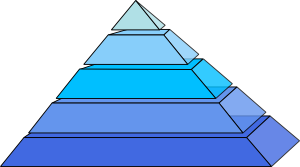
\includegraphics[width=1.1cm]{../Strukturfiler/FIGS/BluePyramid} & \begin{minipage}{\obsl}}{\end{minipage}\\ \end{tabular}\vspace{4mm}\newline}


% = Forudsætning = basis
\newenvironment{basis}{\begin{flushleft} \begin{itshape} }{\end{itshape} \end{flushleft}}


% = Opsummering =
\newenvironment{summary}{\clearpage\pagecolor{sumgul}\section{Opsummering}}{\newpage\pagecolor{white}}











% = Counter
\newcounter{opgavecount}[section]
\setcounter{opgavecount}{0}
\newcounter{spgcount}[opgavecount]
\setcounter{spgcount}{0}
\renewcommand{\thespgcount}{\alph{spgcount})}



% = EXERCISE = (DIVIDER)

\newcommand{\exercisebegin}[1][]{\bigskip\needspace{3\baselineskip}\refstepcounter{opgavecount}\titlegraphic{mingroen}\textcolor{mingroen}{\th{Opgave \theopgavecount \hspace*{1cm} #1}}\medskip\par}

% = QUIZEXERCISE = (DIVIDER)

\newcommand{\quizexercisebegin}[1][]{\bigskip\needspace{3\baselineskip}\refstepcounter{opgavecount}\titlegraphic{mingroen}\textcolor{mingroen}{\th{Quiz-Opgave \theopgavecount \hspace*{1cm} #1}}\medskip\par}

% = QUESTION =

\newenvironment{question}{\refstepcounter{spgcount}\begin{itemize}\item[\thespgcount]}{\end{itemize}\hspace*{\fill}}

% = VINK =

\newenvironment{vink}{\begin{tabular}{m{.9cm}<{\hspace*{2mm}}@{}|m{\obsl}@{}}\hspace*{-4pt}\raggedleft
\includegraphics[width=.9cm]{../Strukturfiler/FIGS/Think} & \begin{minipage}{\obsl}}{\end{minipage}\\ \end{tabular}\medskip\\}
	
% = FACIT =

\newenvironment{facit}{\begin{tabular}{m{.9cm}<{\hspace*{2mm}}@{}|m{\obsl}@{}}\hspace*{-4pt}\raggedleft
\includegraphics[width=.9cm]{../Strukturfiler/FIGS/Check} & \begin{minipage}{\obsl}}{\end{minipage}\\ \end{tabular}\medskip\\}








\newcommand{\afsnit}[1]{\bigskip\th{\titlegraphic{mingroen}\textcolor{mingroen}{#1}} \\ \rule[7pt]{.4\textwidth}{1pt} \vspace*{-2.5mm}\par}

% (DIVIDER):
\newcommand{\ugedagdatotitel}[4]{\pagebreak[4]\section{Semesteruge #1 -- #2 Dag \hspace*{1mm} (#3)} \vspace*{-4mm} \rule[5pt]{\textwidth}{1pt}\vspace*{-2.5mm} \begin{center}\large{\th{#4}}\end{center} \fancyhead[C]{\th{Semesteruge #1}}}

\newenvironment{skema}[1]{\definecolor{shadecolor}{rgb}{0.96,.98, 1.0} \setlength{\FrameSep}{6pt} \renewcommand{\FrameHeightAdjust}{10pt} \vspace*{-4pt}\begin{shaded} \begin{tabular}{#1}}{\end{tabular} \end{shaded} \vspace*{-7pt}}


% ========================

% MAKROER

%\newenvironment{matr}[1][]{\hspace*{-.8mm}\left[\hspace*{-1mm}\begin{array}{#1}}{\end{array}\hspace*{-1mm}\right]\hspace*{-.8mm}}
\newcommand{\bevisslut}{\begin{scriptsize} \begin{flushright} $ \blacksquare $ \end{flushright} \end{scriptsize}}

\newcommand{\tref}[2]{\hyperref[#1]{#2 \ref*{#1}}}
\newcommand{\thref}[2]{\hyperref[#1]{#2}}

\newcommand{\refA}[1]{\colorbox{yellow}{\ref{#1}}}
\newcommand{\hrefA}[2]{\colorbox{yellow}{\href{#1}{#2}}}
\newcommand{\trefA}[2]{\colorbox{yellow}{\hyperref[#1]{#2 \ref*{#1}}}}
\newcommand{\threfA}[2]{\colorbox{yellow}{\hyperref[#1]{#2}}}

\newenvironment{matr}[1]{\hspace*{-.8mm}\begin{bmatrix}\hspace*{-1mm}\begin{array}{#1}}{\end{array}\hspace*{-1mm}\end{bmatrix}\hspace*{-.8mm}}
\newcommand{\transp}{\hspace*{-.6mm}^{\top}}

\newcommand{\maengde}[2]{\left\lbrace \hspace*{-1mm} \begin{array}{c|c} #1 & #2 \end{array} \hspace*{-1mm} \right\rbrace}

\newenvironment{eqnalign}[1]{\setlength{\arraycolsep}{1.3pt}\begin{equation}\begin{array}{#1}}{\end{array}\end{equation}\par}
\newcommand{\eqnl}{\setlength{\arraycolsep}{1.3pt}}

\newcommand{\matind}[3]{{_\mathrm{#1}\mathbf{#2}_\mathrm{#3}}}
\newcommand{\vekind}[2]{{_\mathrm{#1}\mathbf{#2}}}
\newcommand{\jac}[2]{{\mathrm{Jacobi}_\mathbf{#1} (#2)}}
\newcommand{\diver}[2]{{\mathrm{div}\mathbf{#1} (#2)}}
\newcommand{\rot}[1]{{\mathbf{rot}\mathbf{(#1)}}}

\newcommand{\am}{\mathrm{am}}
\newcommand{\gm}{\mathrm{gm}}
\newcommand{\E}{\mathrm{E}}
\newcommand{\Span}{\mathrm{span}}
\newcommand{\mU}{\mathbf{U}}

\newcommand{\ms}{\medskip\\}
\newcommand{\bs}{\bigskip\\}

\newcommand{\mA}{\mathbf{A}}
\newcommand{\mB}{\mathbf{B}}
\newcommand{\mC}{\mathbf{C}}
\newcommand{\mD}{\mathbf{D}}
\newcommand{\mE}{\mathbf{E}}
\newcommand{\mF}{\mathbf{F}}
\newcommand{\mK}{\mathbf{K}}
\newcommand{\mI}{\mathbf{I}}
\newcommand{\mM}{\mathbf{M}}
\newcommand{\mN}{\mathbf{N}}
\newcommand{\mQ}{\mathbf{Q}}
\newcommand{\mT}{\mathbf{T}}
\newcommand{\mV}{\mathbf{V}}
\newcommand{\mW}{\mathbf{W}}
\newcommand{\mX}{\mathbf{X}}
\newcommand{\ma}{\mathbf{a}}
\newcommand{\mb}{\mathbf{b}}
\newcommand{\mc}{\mathbf{c}}
\newcommand{\md}{\mathbf{d}}
\newcommand{\me}{\mathbf{e}}
\newcommand{\mn}{\mathbf{n}}
\newcommand{\mr}{\mathbf{r}}
\newcommand{\mv}{\mathbf{v}}
\newcommand{\mw}{\mathbf{w}}
\newcommand{\mx}{\mathbf{x}}
\newcommand{\mxb}{\mathbf{x_{bet}}}
\newcommand{\my}{\mathbf{y}}
\newcommand{\mz}{\mathbf{z}}
\newcommand{\reel}{\mathbb{R}}
\newcommand{\mL}{\bm{\Lambda}} %Lambda-matrix
\newcommand{\mnul}{\bm{0}}
\newcommand{\trap}[1]{\mathrm{trap}(#1)}
\newcommand{\Det}{\operatorname{Det}}
\newcommand{\adj}{\operatorname{adj}}
\newcommand{\Ar}{\operatorname{Areal}}
\newcommand{\Vol}{\operatorname{Vol}}
\newcommand{\Rum}{\operatorname{Rum}}
\newcommand{\diag}{\operatorname{\bf{diag}}}
\newcommand{\bidiag}{\operatorname{\bf{bidiag}}}
\newcommand{\spanVec}[1]{\mathrm{span}\{#1\}}
\newcommand{\Div}{\operatorname{Div}}
\newcommand{\Rot}{\operatorname{\mathbf{Rot}}}

\newcommand{\Jac}{\operatorname{Jacobi}}
\newcommand{\Tan}{\operatorname{Tan}}
\newcommand{\Ort}{\operatorname{Ort}}
\newcommand{\Flux}{\operatorname{Flux}}
\newcommand{\Cmass}{\operatorname{Cm}}
\newcommand{\Imom}{\operatorname{Im}}
\newcommand{\Pmom}{\operatorname{Pm}}
\newcommand{\IS}{\operatorname{I}}
\newcommand{\IIS}{\operatorname{II}}
\newcommand{\IIIS}{\operatorname{III}}
\newcommand{\Le}{\operatorname{L}}
\newcommand{\app}{\operatorname{app}}
\newcommand{\M}{\operatorname{M}}
\newcommand{\re}{\mathrm{Re}}
\newcommand{\im}{\mathrm{Im}}

\newcommand{\compl}{\mathbb{C}} %de komplekse tal
\newcommand{\e}{\mathrm{e}} %eksponentialfunktionen. lodret 'e', og altså ikke kursiv ligesom andre bogstaver.





% Medialink: SCREEN: (QRcode) + thumbnail image + link på kodenummer (til qr.dtu.dk)
\newcommand{\onlinemedia}[3]{
	\begin{wrapfigure}{r}{3.2cm} 
		\vspace{-30pt} 
		\vspace{#1pt} 
		\begin{flushright} 
			\includegraphics[width=3cm]{qr/#2.png} 
			\tiny 
			\href{http://qr.dtu.dk/#2}{#2: #3}
			\normalsize  
		\end{flushright} 
		\vspace{-10pt} 
	\end{wrapfigure}
}
\newcommand{\onlinemediathumb}[3]{
	\begin{wrapfigure}{r}{3.2cm} 
		\vspace{-30pt} 
		\vspace{#1pt} 
		\begin{flushright} 
			\includegraphics[width=3cm]{qr/#2.png} 
			\includegraphics[width=3cm]{qr/#2_thumb.png} 
			\tiny 
			\href{http://qr.dtu.dk/#2}{#2: #3}
			\normalsize  
		\end{flushright} 
		\vspace{-10pt} 
	\end{wrapfigure}
}



% Index:
\usepackage{makeidx}
\makeindex
\newcommand\ind[2]{\index{#1}\textbf{\textit{\textcolor{black}{#2}}}}

% ###SERVER_EXCLUDE_BEGIN###
\externaldocument[NUID17-]{../../enoten/TN01-Talrum/Talrum}
\externaldocument[NUID1-]{../../enoten/TN02-Ligningssystemer/TNdriver}
\externaldocument[NUID2-]{../../enoten/TN03-Matricer_og_Matrixalgebra/Matricer_og_matrixalgebra}
\externaldocument[NUID3-]{../../enoten/TN04-Kvadratiske_matricer/TNdriver}
\externaldocument[NUID11-]{../../enoten/TN05-Determinanter/Determinanter}
\externaldocument[NUID12-]{../../enoten/TN06-GeometriskeVektorer/GeometriskeVektorer}
\externaldocument[NUID18-]{../../enoten/TN07-Vektorrum/VektorRum}
\externaldocument[NUID21-]{../../enoten/TN08-LinAfbildninger/LinAfbildninger}
\externaldocument[NUID23-]{../../enoten/TN09-Egenvaerdier_og_egenvektorer/TNdriver}
\externaldocument[NUID24-]{../../enoten/TN10-Diagonalisering_med_egenvektorer/TNdriver}
\externaldocument[NUID10-]{../../enoten/TN11-1.ordens_differentialligninger/TNdriver}
\externaldocument[NUID13-]{../../enoten/TN12-1.ordens_differentialligningssystemer/TNdriver}
\externaldocument[NUID14-]{../../enoten/TN13-2.ordens_differentialligninger/TNdriver}
\externaldocument[NUID27-]{../../enoten/TN14-Elemenataere_funktioner/Elementaere_Funktioner}
\externaldocument[NUID28-]{../../enoten/TN15-Funktioner2Variable/Funktioner_To_Variable}
\externaldocument[NUID29-]{../../enoten/TN16-Gradienter_og_Tangentplaner/Gradienter_og_Tangentplaner}
\externaldocument[NUID32-]{../../enoten/TN17-Taylor_formler/Taylor_Formler}
\externaldocument[NUID33-]{../../enoten/TN18-Taylor_2Var/Taylor_2Var}
\externaldocument[NUID34-]{../../enoten/TN19-SymMat/SymmetriskeMatricer}
\externaldocument[NUID35-]{../../enoten/TN20-KegleSnit/Keglesnit}
\externaldocument[NUID36-]{../../enoten/TN21-Riemann_Integral/Riemann_01}
\externaldocument[NUID37-]{../../enoten/TN22-Plan_Int/Plan_Int_01}
\externaldocument[NUID39-]{../../enoten/TN23-Flade_Int/Flade_Rum_Int_01}
\externaldocument[NUID40-]{../../enoten/TN24-Vektorfelter/Vektorfelter_01}
\externaldocument[NUID41-]{../../enoten/TN25-Flux/Flux_02}
\externaldocument[NUID42-]{../../enoten/TN26-Gauss/Gauss_01}
\externaldocument[NUID128-]{../../enoten/TN27-Stokes/Stokes_01}
\externaldocument[NUID43-]{../../enoten/TN29-KomplekseTal/KomplekseTal}

\externaldocument[NUID6-]{../../E-math-opgaver/Opgaver/opgU123}
\externaldocument[NUID19-]{../../E-math-opgaver/Opgaver/opgU45}
\externaldocument[NUID20-]{../../E-math-opgaver/Opgaver/opgU678}
\externaldocument[NUID25-]{../../E-math-opgaver/Opgaver/opgU910SD}
\externaldocument[NUID31-]{../../E-math-opgaver/OpgaverF11-U123/opgF123}
% \externaldocument[NUID9-]{../../E-math-opgaver/Opgaver/Dagsordner E10}
% ###SERVER_EXCLUDE_END###


% Begin document and set alternative chapter title:
\begin{document}
\renewcommand{\chaptername}{eNote}

\setcounter{chapter}{7} %SÆT DETTE TAL TIL 1 MINDRE END DET AKTUELLE TRANSFERNOTE-NUMMER!!

%%%%%%%%%%%%%%%%%%%%%%%%%%%%%%%%%%%%%%%%%%%%%
%%%%%%%%%%%%%%%%%%%%%%%%%%%%%%%%%%%%%%%%%%%%%
%%% HERFRA SKAL DU SKRIVE ELLER INDSÆTTE %%%%
%%% DEN FIL DU ØNSKER %%%%%%%%%%%%%%%%%%%%%%%
%%%%%%%%%%%%%%%%%%%%%%%%%%%%%%%%%%%%%%%%%%%%%
%%%%%%%%%%%%%%%%%%%%%%%%%%%%%%%%%%%%%%%%%%%%%
\chapter{Lineære Afbildninger} \label{tn8}

\begin{basis}
Denne eNote undersøger en vigtig type af afbildninger mellem vektorrum, nemlig lineære afbildninger. Det vises at kernen og billedrummet for lineære afbildninger er underrum i henholdsvis definitionsrummet og dispositionsrummet. Når der er valgt basis i definitionsrummet og i dispositionsrummet, kan spørgsmål vedrørende lineære afbildninger standardiseres, idet en lineær afbildning udtrykkes som et produkt mellem en såkaldt afbildningsmatrix og koordinaterne for de vektorer der ønskes afbildet. Da afbildningsmatricer afhænger af de to valgte baser, beskrives det hvordan afbildningsmatricerne ændres når en af baserne eller de begge udskiftes med andre. Forudsætninger for eNoten er viden om lineære ligningssystemer, se \tref{NUID1-tn2}{eNote}, matrixalgebra, se \tref{NUID2-tn3}{eNote} og vektorrum, se \tref{NUID18-tn7}{eNote}.
\end{basis}

\section{Om afbildninger}
En afbildning er en forskrift $f$ der til et element i en mængde $A$ knytter et element i en mængde $B$, og forskriften skrives $\,f:A\rightarrow B\,$. $A$ kaldes \ind{definitionsmængde}{definitionsmængden} og $B$ \ind{dispositionsmængde}{dispositionsmængden}.\bs
CPR-nummerering er en afbildning af mængden af statsborgere i Danmark ind i $\,\mathbb R^{10}\,$. Bemærk at der er en 10-dobbelt uendelig af elementer i dispositionsmængden $\,\mathbb R^{10}\,$, så vi har  heldigvis kun brug for en meget lille delmængde af dem, ca. fem millioner! De elementer i $\,\mathbb R^{10}\,$ som på et givet tidspunkt er i brug, er \ind{billedmængde}{billedmængden} for CPR-afbildningen.\bs   
En enkel type af afbildninger er elementære funktioner af typen $\,f:\,\mathbb R \rightarrow \mathbb R\,.$ Pilen udtrykker her at $\,f\,$ til ethvert reelt tal $x$ knytter et andet reelt tal $y=f(x)\,$. Betragt for eksempel den kontinuerte funktion:
\begin{equation}\label{funktion}
y=f(x)=\,\frac 12\,x^2-2\,.
\end{equation}
Her har forskriften form af en regneprocedure: Sæt tallet i anden, gang det med en halv og træk 2 fra. Elementære funktioner har en stor fordel ved at deres graf $\,\left\{\,(x,y)\,|\,y=f(x)\,\right\}\,$ kan tegnes og give et særligt overblik over afbildningen:
\begin{center}
		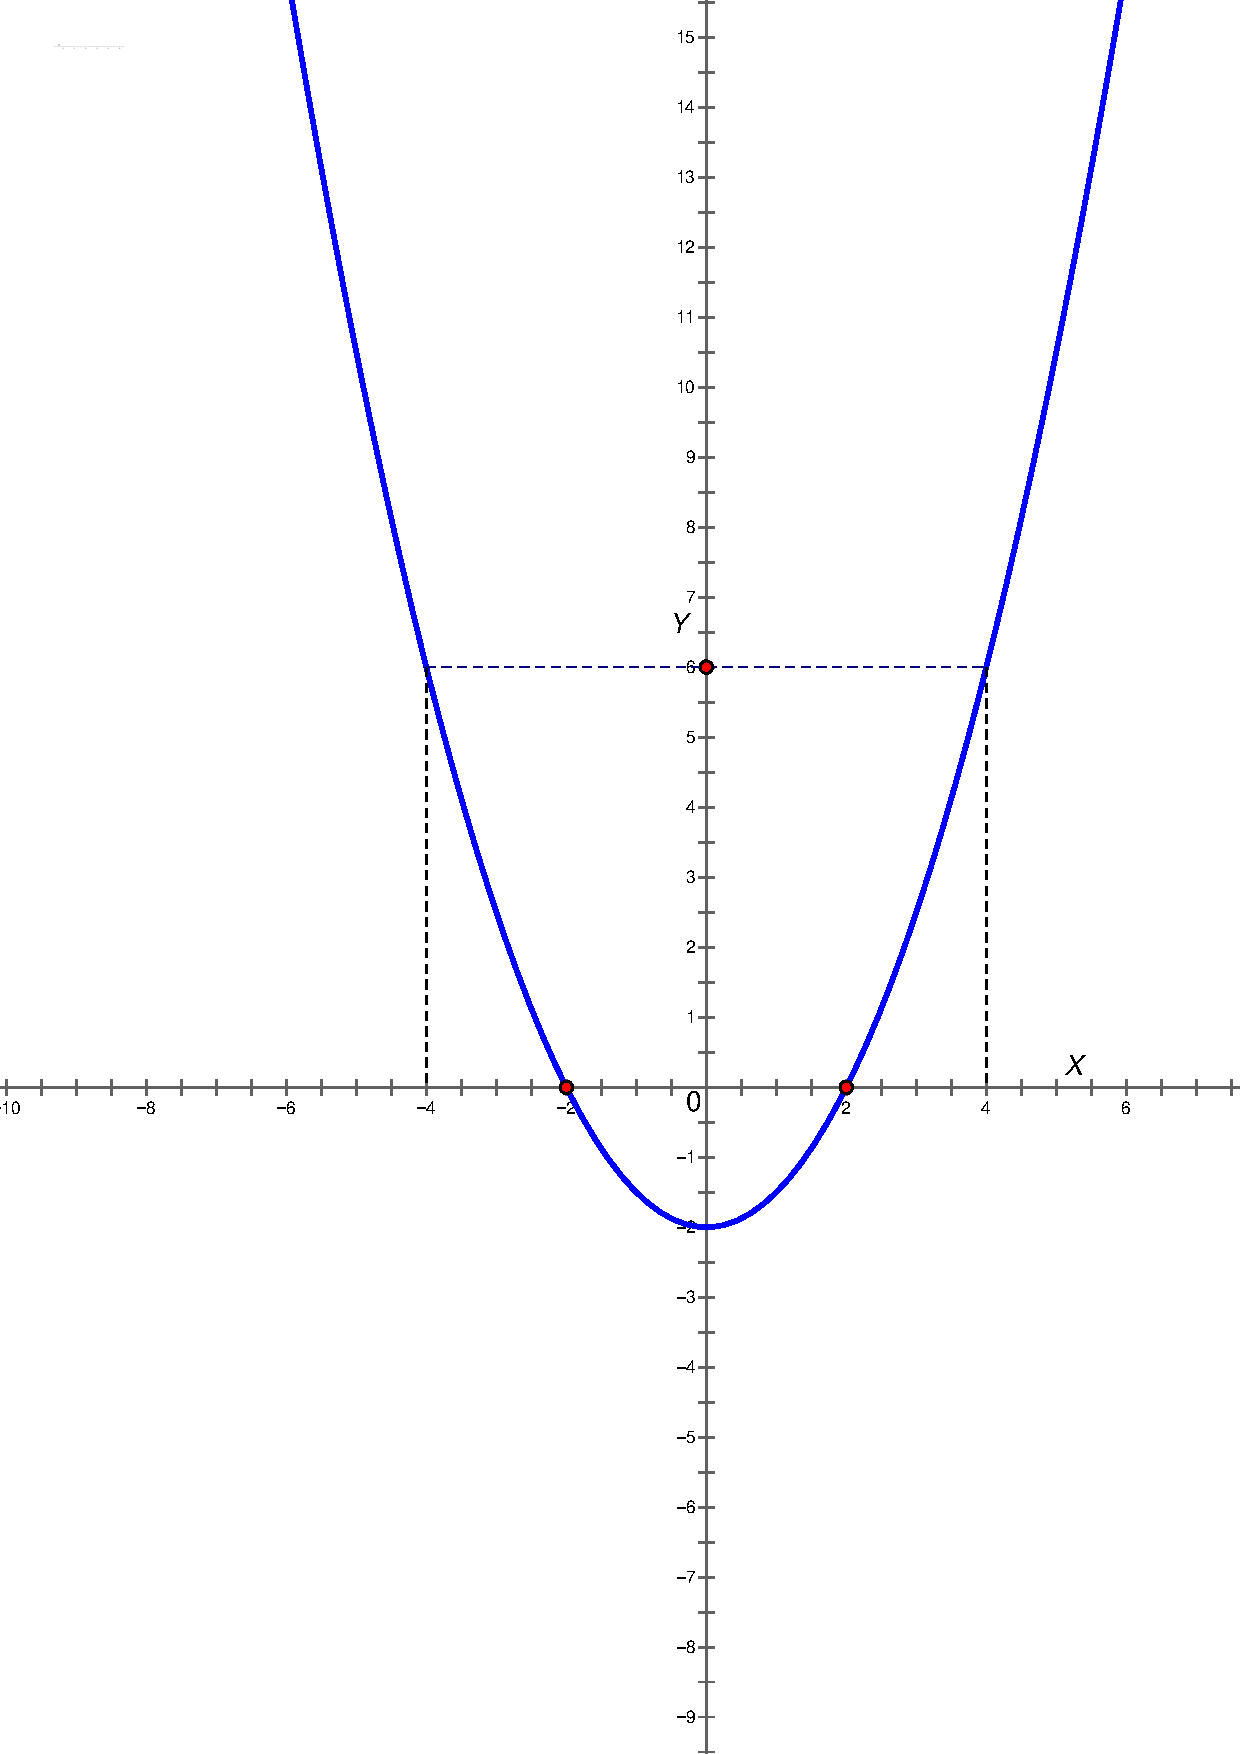
\includegraphics[trim=5.5cm 8.5cm 3cm
 9.5cm,width=0.45\textwidth,clip]{graf.pdf}
  \\Figur 8.1: Graf for elementær funktion%$y=f(x)=\,\frac12\,x^2-2\,.$		
\end{center}

Typiske spørgsmål i forbindelse med elementære funktioner, kommer igen i forbindelse med mere avancerede afbildninger. Lad os derfor indledningsvist kigge på nogle af de vigtigste:
\begin{enumerate}
\item
Bestem nulpunkterne for $f\,$. Det betyder at vi skal finde alle $x$ for hvilke $f(x)=0$. I eksemplet er svaret $x=-2$ og $x=2$. 
\item
Løs for et givet $b$ ligningen $f(x)=b\,$. For $b=6$ er der i eksemplet to løsninger: $x=-4$ og $x=4\,.$ 
\item
Bestem billedmængden (= værdimængden) for $f\,$. Vi skal finde alle de $b$ for hvilke ligningen $f(x)=b\,$ har en løsning. I eksemplet er billedmængden $\left[\,-2;\infty\,\right[$.
\end{enumerate}

I denne eNote ser vi på defintionsmængder, dispositionsmængder og billedmængder som er \textit{vektorrum}. Derfor præciseres mængdebegreberne til definitions\textit{rum}, dispositions\textit{rum} og billed\textit{rum}. En afbildning $\,f:V \rightarrow W\,$ knytter til enhver vektor $\mathbf x$ i \textit{definitionsrummet}  $V$ en vektor $\mathbf y=f(\mathbf x)$ i \textit{dispositionsrummet} $W\,$. Alle de vektorer i $W\,$ som er billede af en vektor i $V\,$ udgør \textit{billedrummet}.

\begin{example}[Afbildning fra vektorrum til vektorrum]\label{tn8.ex0_linAfb}
En afbildning $\,g:\mathbb R^{2\times 3}\rightarrow \mathbb R^{2\times 2}$ er givet ved
\begin{equation}
\mathbf Y = g(\mathbf X)=\mathbf X\,\mathbf X\transp\,.
\end{equation}
Der gælder for eksempel at 
$$g\Big (\begin{matr}{lll}1&0&2\\0&3&0\end{matr}\Big)
=\begin{matr}{lll}1&0&2\\0&3&0\end{matr}\,
\begin{matr}{ll}1&0\\0&3\\2&0\end{matr}
=\begin{matr}{ll}5&0\\0&9\end{matr}\,.$$
\end{example}

\section{Eksempler på lineære afbildninger i planen}

Vi undersøger i det følgende en afbildning $f\,$ der har mængden af geometriske vektorer i planen som både definitionsrum og dispositionsrum. For en given geometrisk vektor $\mx$ vil vi ved $\hat{\mathbf x}$ forstå dens \textit{tværvektor}. Afbildningen $f$ er da givet ved  
\begin{equation}
\mathbf y =f(\mathbf x)=2\,\hat{\mathbf x}\,.
\end{equation}
Til enhver vektor i planen er der altså knyttet dens tværvektor multipliceret (forlænget) med 2. På figur 8.2\, er der tegnet to vektorer $\mathbf u$ og $\mathbf v$ og deres billeder $f(\mathbf u)$ og $f(\mathbf v)$.

\begin{center}
		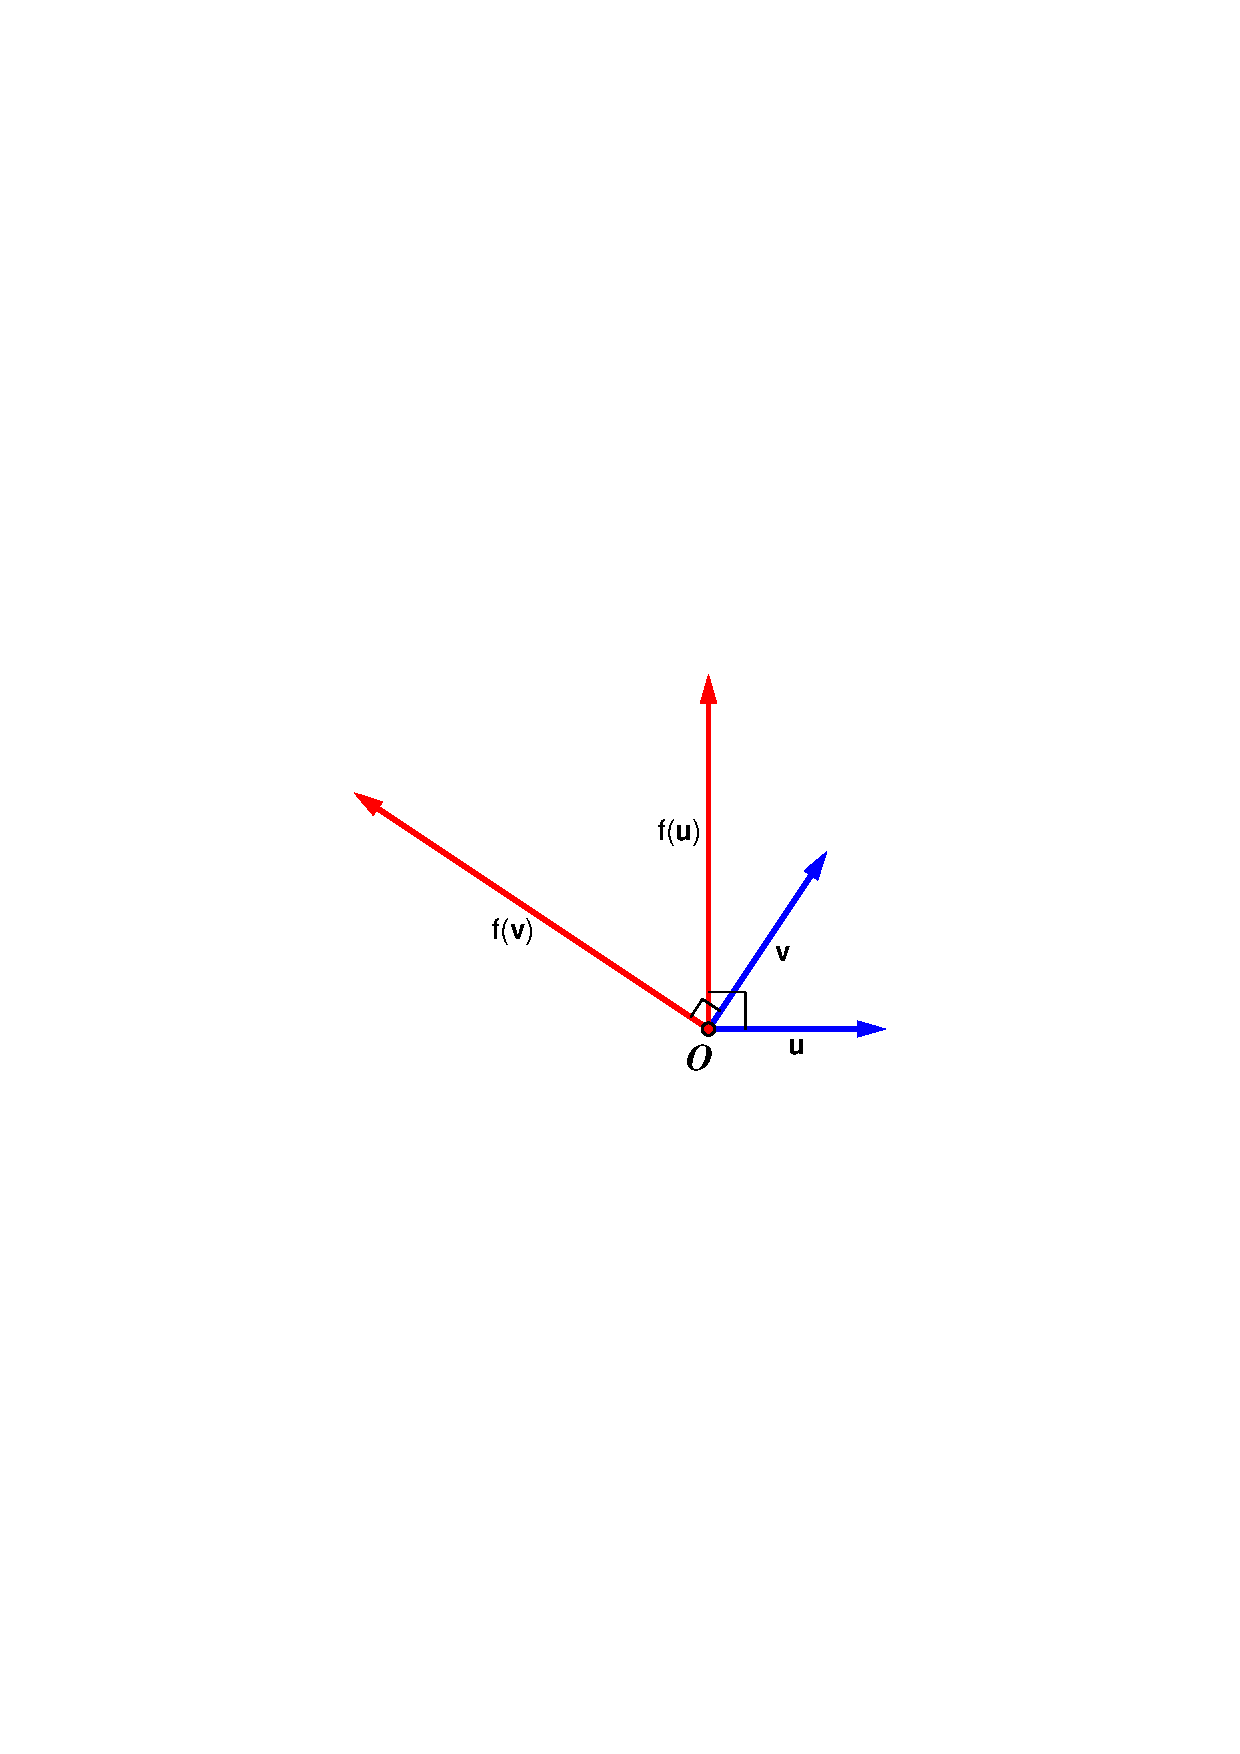
\includegraphics[trim=5cm 11cm 5cm
 11cm,width=0.40\textwidth,clip]{tvarVektor2.pdf}
  \\Figur 8.2: To vektorer (blå) og deres billeder (røde). 
\end{center}

Figur 8.2 giver anledning til et par interessante spørgsmål: Hvordan afbildes sumvektoren $\mathbf u +\mathbf v\,$? Mere præcist: Hvordan forholder billedvektoren $f(\mathbf u + \mathbf v)$ sig til de to billedvektorer $f(\mathbf u)$ og $f(\mathbf v)$? Og hvad er relationen mellem billedvektorerne $f(k\mathbf u)$ og  $f(\mathbf u)\,,$ når $k$ er er givet reelt tal?

\begin{center}
\begin{tabular}{cc}

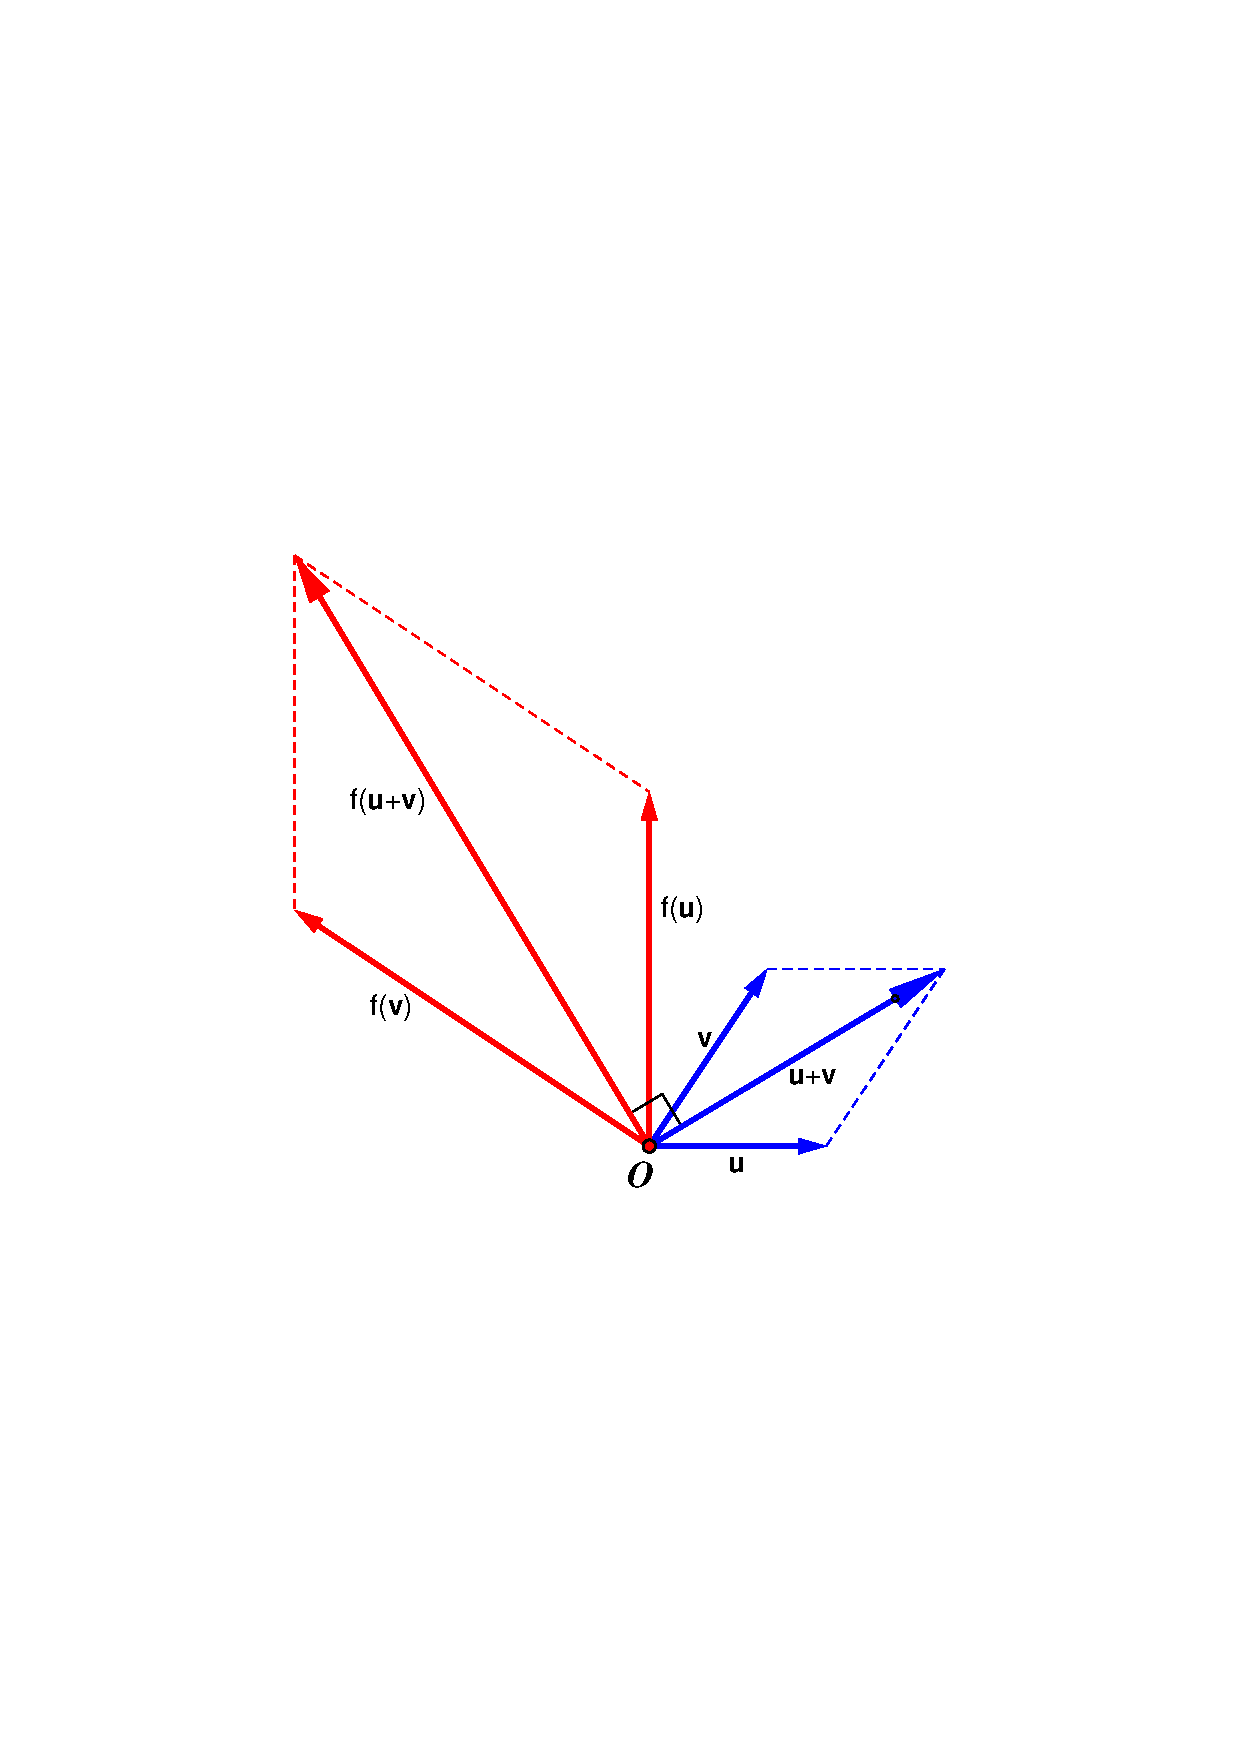
\includegraphics[trim=5cm 9.6cm 5cm
 9.5cm,width=0.40\textwidth,clip]{tvarVektor3.pdf}
&
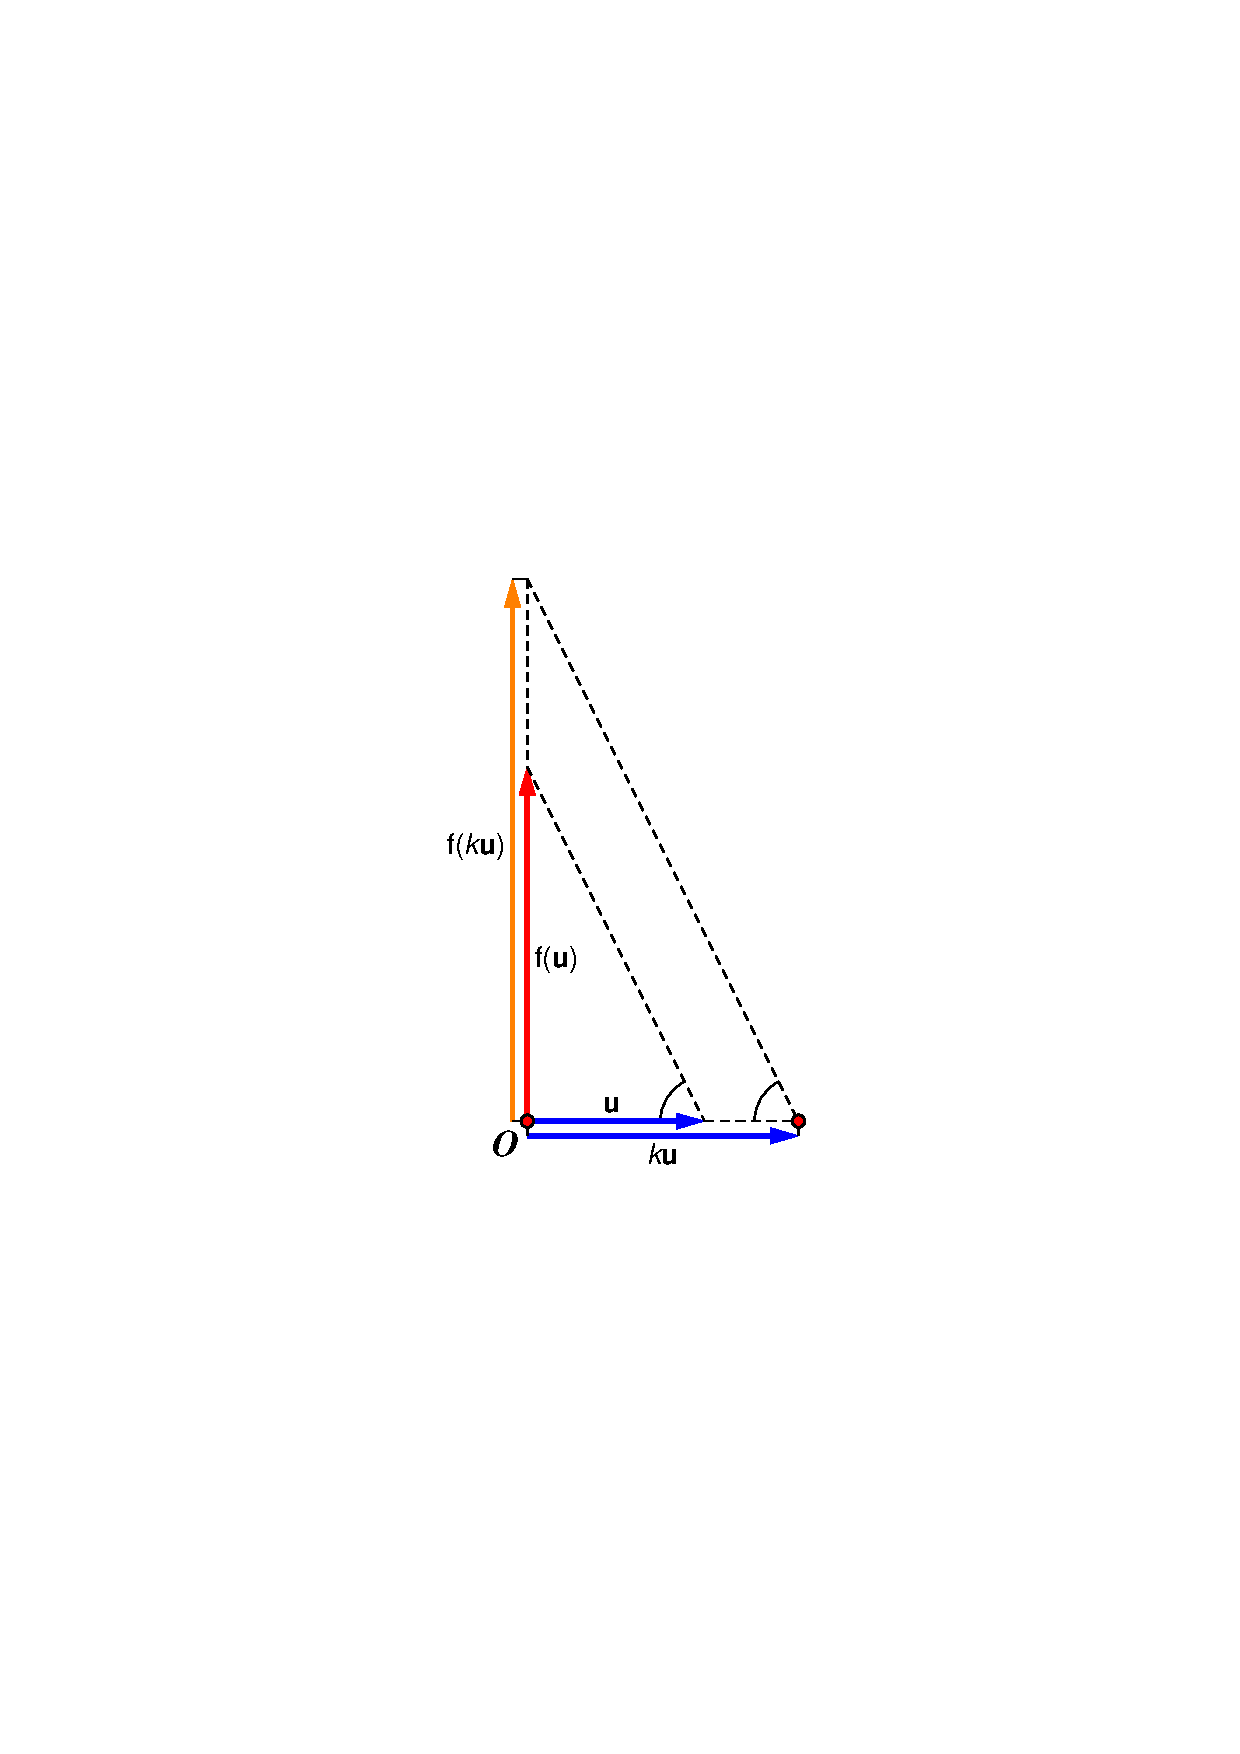
\includegraphics[trim=5cm 9.6cm 5cm
 9.5cm,width=0.40\textwidth,clip]{tvarVektor4.pdf}
\end{tabular}

Figur 8.3: Konstruktion af $f(\mathbf u + \mathbf v)$ og $f(k\mathbf u)\,.$

\end{center}

Som antydet på figur 8.3\, opfylder $f$ to meget enkle regler:
\begin{equation}\label{tn8.ex1_linAfb}
f(\mathbf u + \mathbf v)=f(\mathbf u) + f(\mathbf v) 
\,\,\,\mathrm{og}\,\,\,f(k\mathbf u)=k\,f(\mathbf u)\,.
\end{equation}

Ved hjælp af af de velkendte regneregler for tværvektorer
\begin{enumerate}
\item
$\widehat{\mathbf u + \mathbf v}=\hat{\mathbf u} + \hat{\mathbf v}$.
\item
$\widehat{k\mathbf u}=k\hat{\mathbf u}\,.$
\end{enumerate}
kan vi nu bekræfte påstanden (\ref{tn8.ex1_linAfb})\,:
\begin{align*}
f(\mathbf u + \mathbf v)&=2\widehat{\mathbf u + \mathbf v}=2(\hat{\mathbf u} + \hat{\mathbf v})=2\hat{\mathbf u} + 2\hat{\mathbf v}\\&=f(\mathbf u) + f(\mathbf v)\,.\\
f(k\mathbf u)&=2\widehat{k\mathbf u}=2k\hat{\mathbf u}=k(2\hat{\mathbf u})\\&
=k\,f(\mathbf u)\,.
\end{align*}

\begin{exercise}
En afbildning $f_1$ af plane vektorer er givet ved $f_1(\mv)=3\mv$, se figur 8.4:
\begin{center}
		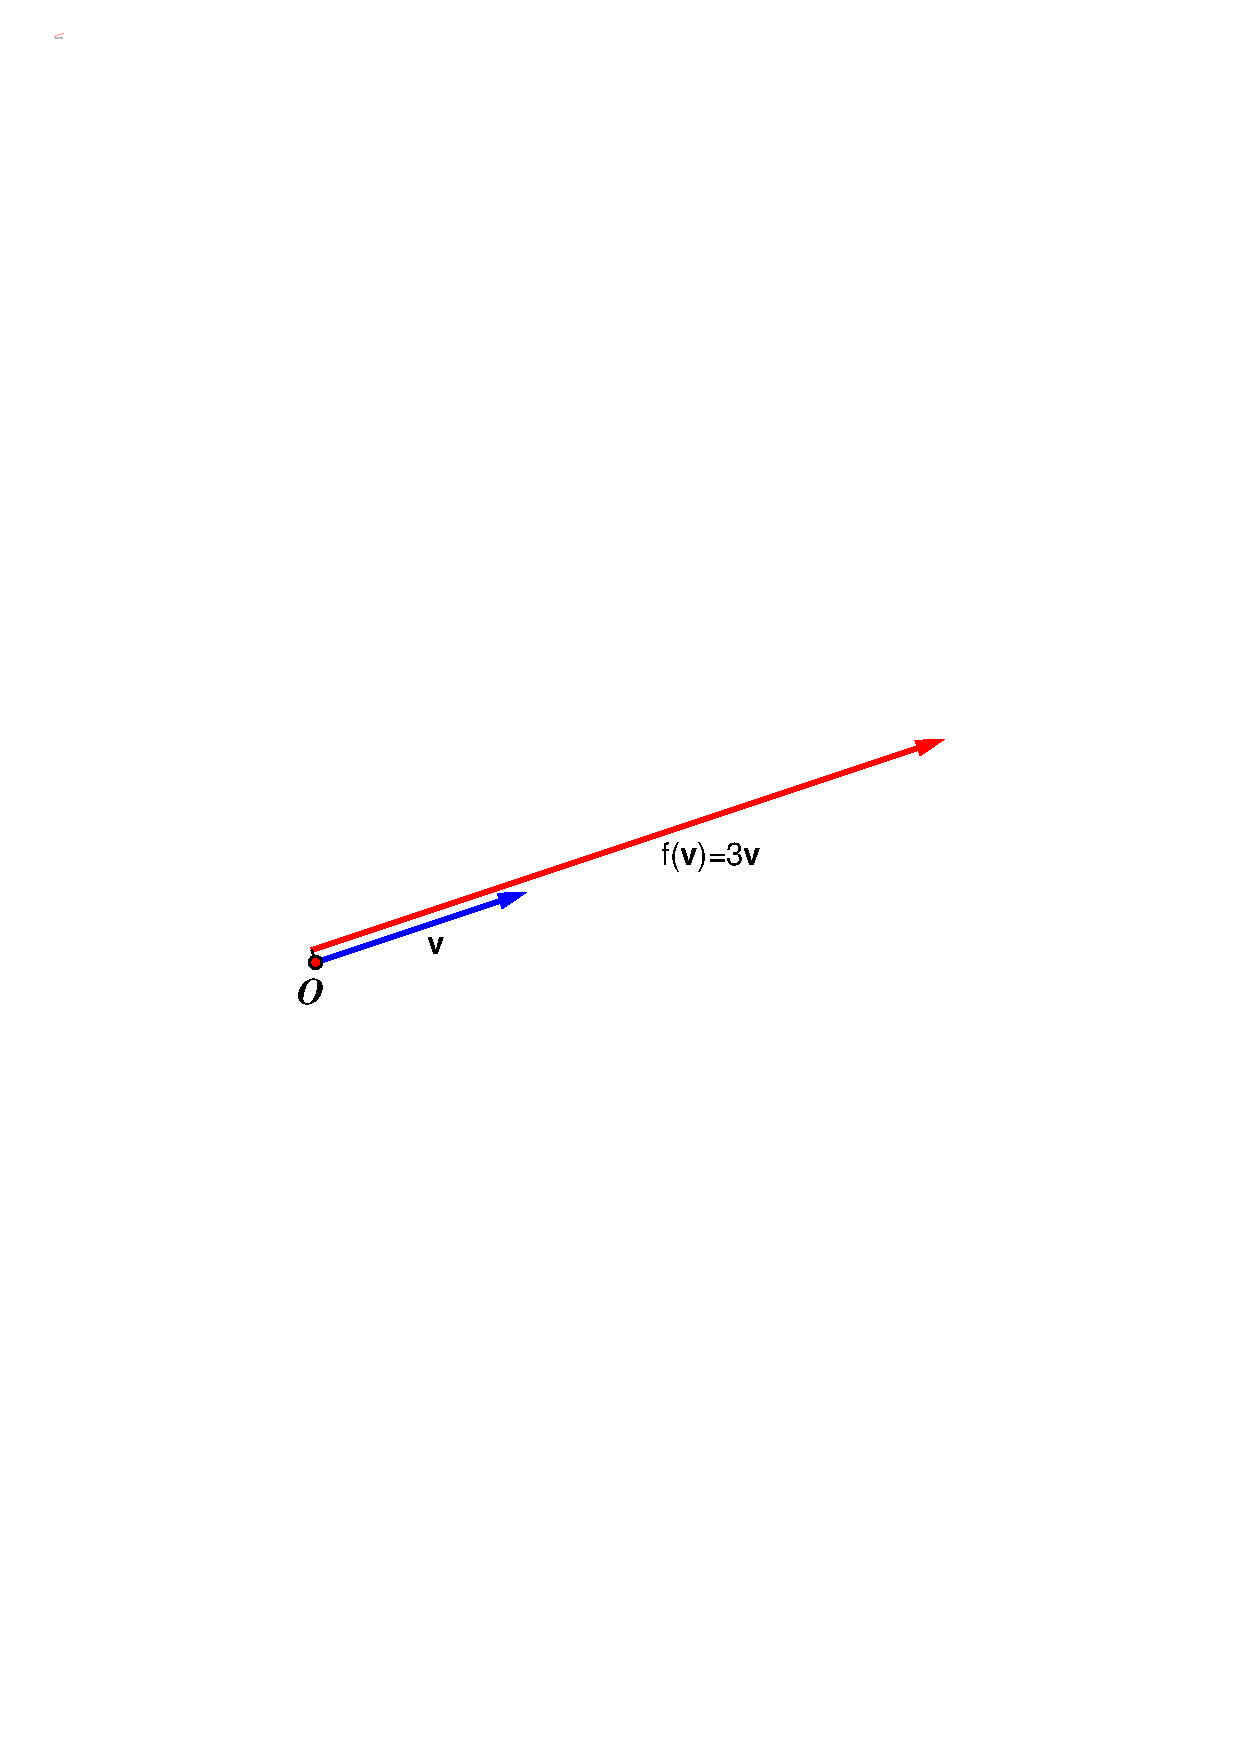
\includegraphics[trim=5cm 12cm 5cm
 12cm,width=0.40\textwidth,clip]{skalering.pdf}
  \\Figur 8.4: Skalering af vektor 
\end{center}
Tegn en figur der demonstrerer at $f_1$ opfylder reglerne (\ref{tn8.ex1_linAfb})\,.
\end{exercise}

\begin{exercise}
I planen er der givet en linje $l$ gennem Origo. En afbildning $f_2$ spejler vektorer afsat ud fra Origo i $l\,$, se figur 8.5:
\begin{center}
		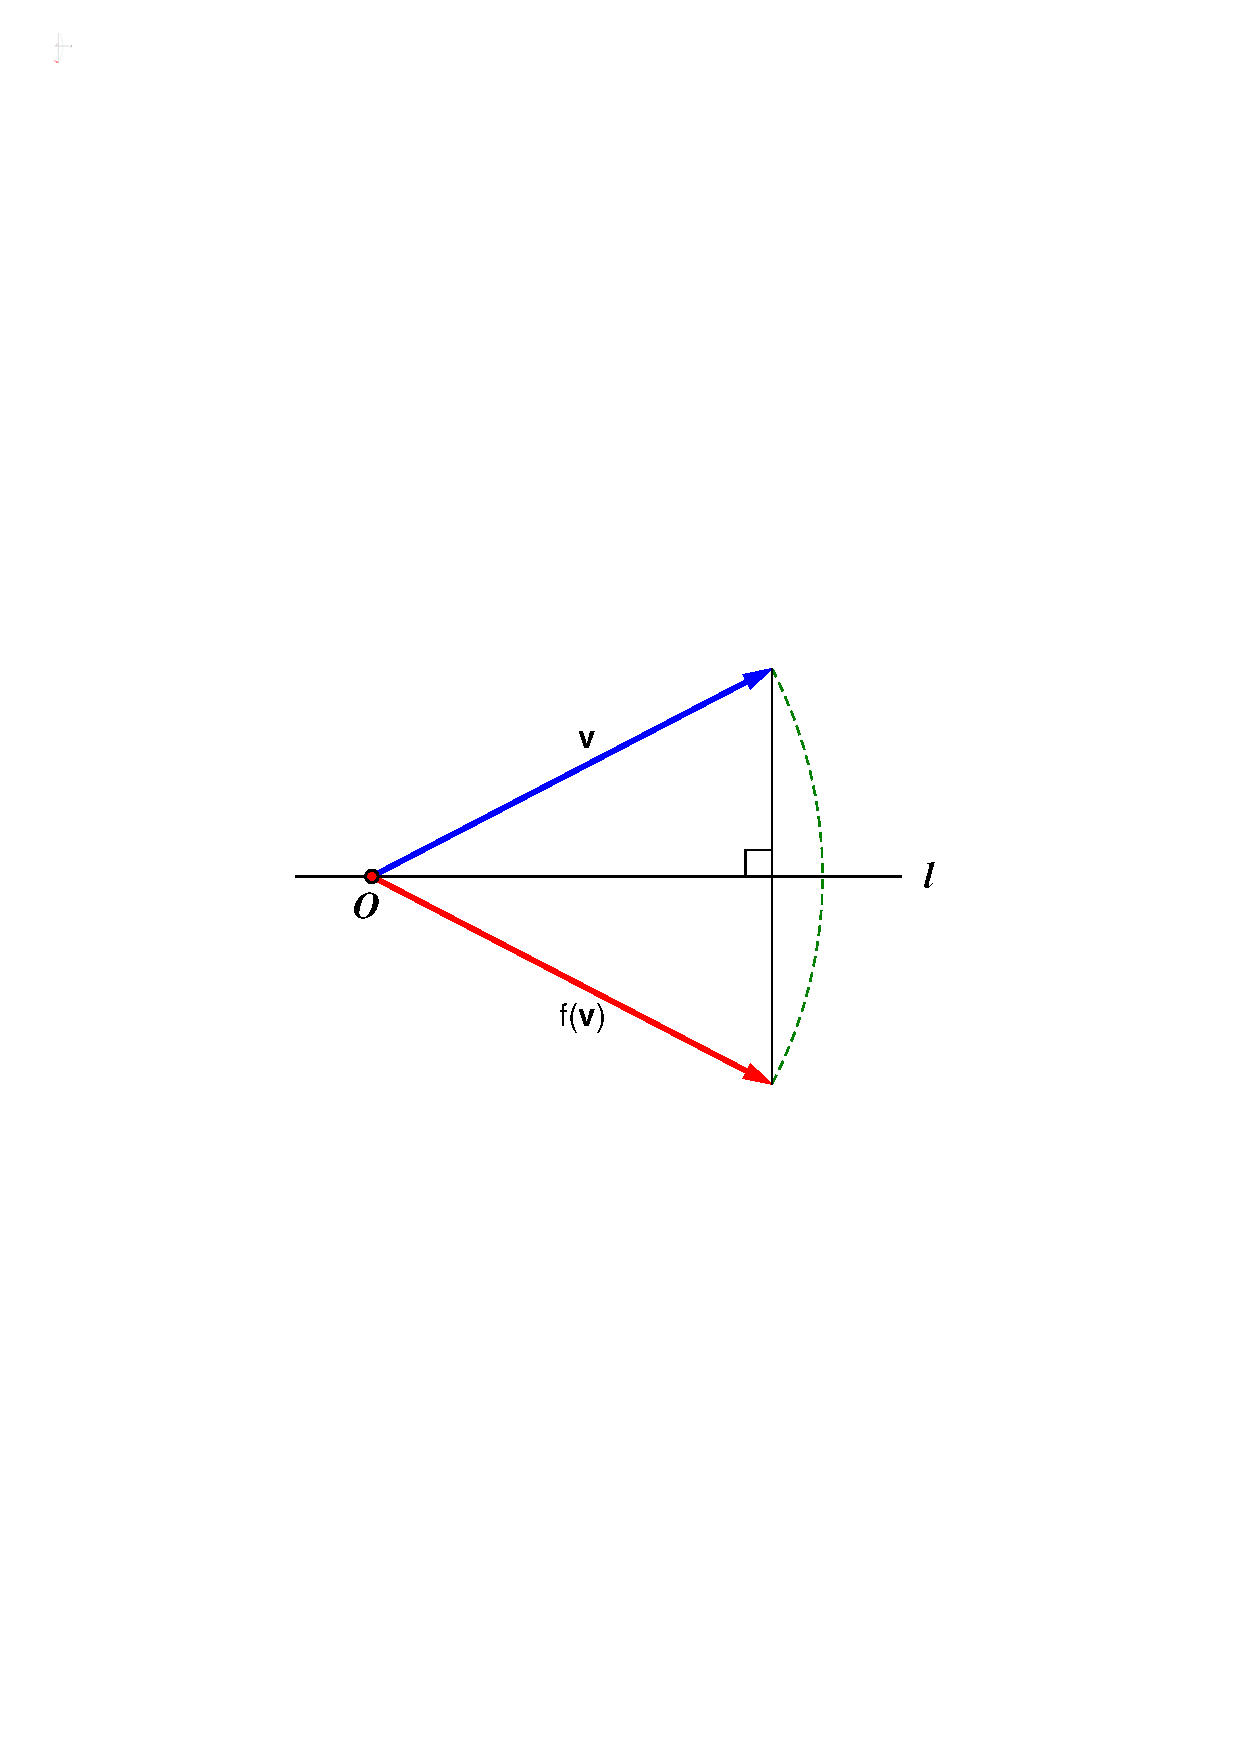
\includegraphics[trim=5cm 11cm 5cm
 11cm,width=0.40\textwidth,clip]{spejling.pdf}
  \\Figur 8.5: Spejling af vektor 
\end{center}
Tegn en figur der demonstrerer at $f_2$ opfylder reglerne (\ref{tn8.ex1_linAfb})\,.
\end{exercise}

\begin{exercise}\label{tn8.opgDrejning}
En afbildning $f_3$ drejer vektorer afsat ud fra Origo vinklen $t$ omkring Origo mod uret, se figur 8.6:
\begin{center}
		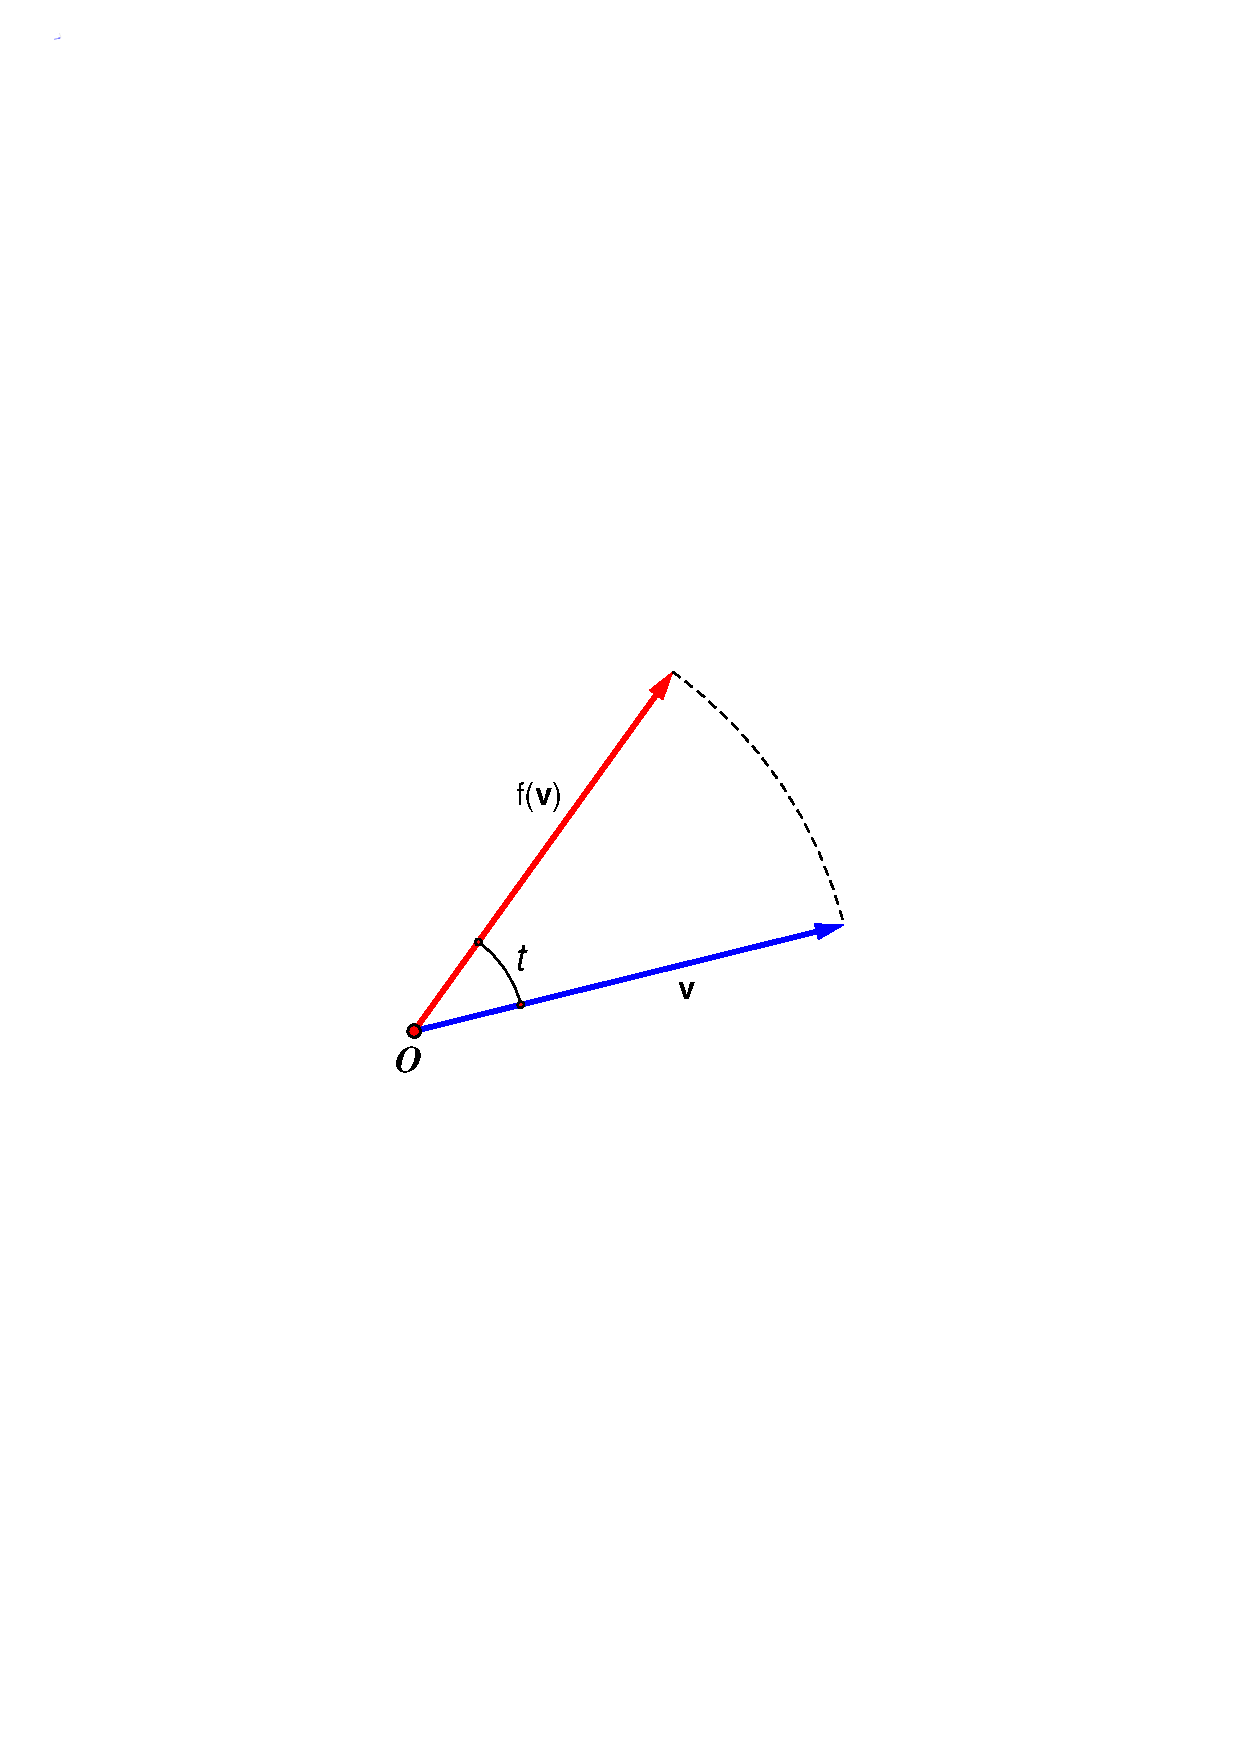
\includegraphics[trim=5cm 11cm 5cm
 11cm,width=0.40\textwidth,clip]{drejNY.pdf}
  \\Figur 8.6: Drejning af vektor 
\end{center}
Tegn en figur der demonstrerer at $f_3$ opfylder reglerne (\ref{tn8.ex1_linAfb})\,.
\end{exercise}

Alle afbildninger der har været berørt i dette afsnit er \textit{lineære}, fordi de opfylder (\ref{tn8.ex1_linAfb})\,. Vi tager nu spørgsmålet om lineære afbildninger mellem vektorrum op til generel behandling.

\section{Lineære afbildninger}

\begin{definition}[Lineær afbildning]\label{tn8.def_linAfb}
Lad $V$ og $W$ være to vektorrum. En afbildning $\,f:V\rightarrow W\,$ kaldes \ind{lineær}{lineær} hvis den for alle $\mathbf u,\mathbf v \in V$ og alle skalarer $k$ opfylder de følgende to \textit{linearitetsbetingelser}:\bs
\begin{tabular}{ll}
$L_1:$&$f(\mathbf u + \mathbf v)=f(\mathbf u) + f(\mathbf v)\,.$\\
$L_2:$&$f(k\mathbf u)=k\, f(\mathbf u)\,.$
\end{tabular}\bs
$V$ kaldes \textit{definitionsrummet} og $W$ \textit{dispositionsrummet} for $f\,$.
\end{definition}
\begin{aha}
Ved at sætte $k=0$ i linearitetsbetingelsen $\,L_2\,$ i definition \ref{tn8.def_linAfb}\,, ses det at
\begin{equation}
f(\mnul)=\mnul\,.
\end{equation}
Der gælder med andre ord for enhver lineær afbildning $\,f:V\rightarrow W\,$ at nul-vektoren i $V$ afbildes i nul-vektoren i $W\,$.
\end{aha}
\begin{aha}
Billedet af en linearkombination bliver på en meget enkel måde en linearkombination af billederne af de vektorer der indgår i den givne linearkombination:
\begin{equation}\label{tn8.billedLinkomb}
f(k_1\mv_1+k_2\mv_2+\ldots+k_p\mv_p)=
k_1f(\mv_1)+k_2f(\mv_2)+\ldots+k_pf(\mv_p)\,.
\end{equation}
Dette resultat fås ved gentagen anvendelse af $L_1$ og $L_2$.
\end{aha}

\begin{example}[Lineær afbildning] \label{tn8.exL1L2_1}
En afbildning $\,f:\mathbb R^2\rightarrow \mathbb R^4\,$ er givet ved forskriften
\begin{equation}
f(x_1,x_2)=(0,x_1,x_2,x_1+x_2)\,.
\end{equation}
$\reel^2$ og $\reel^4$ er vektorrum, og vi undersøger om $f$ er en lineær vektorrumsafbildning? Vi tester først venstresiden og højresiden af $L_1$ med vektorerne $(1,2)$ og $(3,4)$:
\begin{align*}
f(\,(1,2)+(3,4)\,)&=f(4,6)=(0,4,6,10)\,.\\
f(1,2)+f(3,4)&=(0,1,2,3)+(0,3,4,7)=(0,4,6,10)\,.
\end{align*}
Dernæst testes $L_2$ med vektoren (2,3) og skalaren 5:
\begin{align*}
f(\,5\cdot(2,3)\,)&=f(10,15)=(0,10,15,25)\,.\\
5\cdot f(2,3)&=5\cdot(0,2,3,5)=(0,10,15,25)\,.
\end{align*}
Undersøgelsen tyder på at $f$ er lineær. Dette vises nu generelt. Først testes $L_1$:
\begin{align*}
f(\,(x_1,x_2)+(y_1,y_2)\,)&=f(x_1+y_1,x_2+y_2)=(0,x_1+y_1,x_2+y_2,x_1+x_2+y_1+y_2)\,.\\
f(x_1,x_2)+f(y_1,y_2)&=(0,x_1,x_2,x_1+x_2)+(0,y_1,y_2,y_1+y_2)\\&=(0,x_1+y_1,x_2+y_2,x_1+x_2+y_1+y_2)\,.
\end{align*}
Dernæst testes $L_2$:
\begin{align*}
f(\,k\cdot(x_1,x_2)\,)&=f(k\cdot x_1,k\cdot x_2)=(0,k\cdot x_1,k\cdot x_2,k\cdot x_1+k\cdot x_2)\,.\\
k\cdot f(x_1,x_2)&=k\cdot(0,x_1,x_2,x_1+x_2)=(0,k\cdot x_1,k\cdot x_2,k\cdot x_1+k\cdot x_2)\,.
\end{align*}
Det ses at $f$ opfylder begge linearitetsbetingelser og derfor er lineær.
\end{example}

\begin{example}[Afbildning som ikke er lineær] \label{tn8.ex2_linAfb}
I eksempel \ref{tn8.ex0_linAfb} betragtede vi afbildningen $\,g:\mathbb R^{2\times 3}\rightarrow \mathbb R^{2\times 2}$ givet ved
\begin{equation}
\mathbf Y = g(\mathbf X)=\mathbf X\,\mathbf X\transp\,.
\end{equation}
At denne afbildning \textit{ikke} er lineær, kan man dokumentere ved at finde et eksempel hvor enten $L_1$ eller $L_2$ ikke gælder. Nedenfor gives et eksempel på en matrix $\mathbf X$ som ikke opfylder $\,g(2\mathbf X)=2\,g(\mathbf X)\,$:   

$$g\Big (2\begin{matr}{lll}1&0&0\\0&0&0\end{matr}\Big)
=g\Big (\begin{matr}{lll}2&0&0\\0&0&0\end{matr}\Big)
=\begin{matr}{lll}2&0&0\\0&0&0\end{matr}\,
\begin{matr}{ll}2&0\\0&0\\0&0\end{matr}
=\begin{matr}{ll}4&0\\0&0\end{matr}\,.$$
Men
$$2\,g\Big (\begin{matr}{lll}1&0&0\\0&0&0\end{matr}\Big)
=2\begin{matr}{lll}1&0&0\\0&0&0\end{matr}\,
\begin{matr}{ll}1&0\\0&0\\0&0\end{matr}
=2\begin{matr}{ll}1&0\\0&0\end{matr}
=\begin{matr}{ll}2&0\\0&0\end{matr}\,.$$
Derfor opfylder $g$ ikke linearitetsbetingelse $L_2$, og $g$ er derfor ikke lineær.
\end{example}

\begin{example}[Lineær afbildning]\label{tn8.ex3Linafb}
Der er givet en afbildning $f:P_2(\mathbb R) \rightarrow \mathbb R$ ved forskriften
\begin{equation}
f\big(\,P(x)\,\big)=P'(1)\,.
\end{equation}
Til ethvert andengradspolynomium er altså knyttet dets tangenthældning i $\,x=1\,$. Et vilkårligt andengradspolynomium $P$ kan opskrives ved $P(x)=a x^2+b x+c$. Da $\,P'(x)=2ax+b\,$ har vi:
$$f\big(\,P(x)\,\big)=2a+b\,.$$
Hvis vi sætter $P_1(x)=a_1x^2+b_1x+c_1$ og
$P_2(x)=a_2 x^2+b_2 x+c_2\,$, får vi
\begin{align*}
f\big(\,P_1(x)+P_2(x)\,\big)&=
f\big(\,(a_1+a_2)x^2+(b_1+b_2)x+(c_1+c_2)\,\big)\\&=
\big(\,2(a_1+a_2)+(b_1+b_2)\,\big)\\&=(2a_1+b_1)+(2a_2+b_2)\\&=
f\big(\,P_1(x)\,\big)+f\big(\,P_2(x)\,\big)\,.
\end{align*}
Endvidere for ethvert reelt tal $k$ og ethvert andengradspolynomium $P(x)$:
\begin{align*}
f\big(\,k\cdot P(x)\,\big)&=f\big(\,k\cdot ax^2+k\cdot bx+k\cdot c\,\big)\\&=(2k\cdot a+k\cdot b)=k\cdot(2a+b)\\&=k\cdot f\big(\,P(x)\,\big)\,.
\end{align*}
Det er hermed vist at $f$ opfylder linearitetsbetingelserne $L_1$ og $L_2\,$, og at $f$ dermed er en lineær afbildning.
\end{example}

\begin{exercise}
Ved $C^{\infty}(\mathbb R)$ forstås vektorrummet som består af alle funktioner $\,f:\mathbb R\rightarrow \mathbb R\,$ som kan differentieres et vilkårligt antal gange. Et eksempel (blandt uendeligt mange) er funktionen $f(x)=\sin(x)$. Betragt afbildningen $\mathrm D:C^{\infty}(\mathbb R)\rightarrow C^{\infty}(\mathbb R)$ som til en funktion $f(x)\in C^{\infty}(\mathbb R)$ knytter dens afledede:
$$\mathrm D\big(\,f(x)\,\big)=f'(x)\,.$$
Vis at $\mathrm D$ er en lineær afbildning. 
\end{exercise}
%\end{document}
\section{Kerne og billedrum}
Nulpunkterne for en elementær funktion $f:\mathbb R\rightarrow \mathbb R$ er alle de reelle tal $x$ som opfylder $f(x)=0\,$. Det tilsvarende begreb for lineære afbildninger kaldes \textit{kernen}. Billedmængden (eller værdimængden) for en elementær funktion $f:\mathbb R\rightarrow \mathbb R$ er alle de reelle tal $b$, hvortil der findes et reelt tal $x$ således at $f(x)=b\,$. Det tilsvarende begreb for lineære afbildninger kaldes \textit{billedrummet}. Lad os straks retfærdiggøre at ordet \textit{rum} optræder her. Kernen er et underrum i definitionsrummet og billedrummet er et underrum i dispositionsrummet. Dette vil blive uddybet nedenfor.

\begin{definition}[Kerne og billedrum]\label{tn8.defKerne}
Ved \ind{kerne}{kernen} for en lineær afbildning $\,f:V\rightarrow W\,$ forstås mængden:
\begin{equation}
\ker(f)=\left\{\,\mathbf x\in V\,|\,\,f(\mathbf x)=\mnul\in W\,\right\}\,.  
\end{equation}
Ved \ind{billedrum}{billedrummet} for $f$ forstås mængden:  
\begin{equation}\label{tn8_bildrum}
f(V)=\left\{\,\mathbf b\in W\,|\,\mathrm{Der\,\,findes\,\,mindst\,\,et}\,\, \mathbf x \in V\,\,\mathrm{hvor} \,\,f(\mathbf x)=\mb\,\right\}\,.
\end{equation}
\end{definition}

\begin{theorem}[Kernen og billedrummet er underrum]\label{tn8.thKernUrum}
Lad $\,f:V\rightarrow W\,$ være en lineær afbildning. Der gælder:
\begin{enumerate}
\item
Kernen for $f$ er et underrum i $V\,$.
\item
Billedrummet $f(V)$ er et underrum i $W\,$.  
\end{enumerate}
\end{theorem}

\begin{bevis}
1) Vi skal vise at kernen for $f$ opfylder stabilitetskravene, se \tref{NUID18-tn7.stabilNok}{sætning}. Antag at $\mathbf x_1 \in V$ og $\mathbf x_2 \in V$, og at $k$ er en vilkårlig skalar. Da der (med brug af $\,L_1\,$) gælder:
$$f(\mathbf x_1+\mathbf x_2)=f(\mathbf x_1)+f(\mathbf x_2)=\mnul+\mnul=\mnul\,,$$
er kernen for $f$ stabil med hensyn til addition. Da der endvidere (med brug af $\,L_2\,$) gælder:
$$
f(k\mathbf x_1)=k\,f(\mathbf x_1)=k\,\mnul=\mnul\,,$$
er kernen for $f$ også stabil med hensyn til multiplikation med skalar. Samlet er det dermed vist at kernen for $f$ er et underrum i $V\,$. \bs
2) Vi skal vise at billedrummet $f(V)$ opfylder stabilitetskravene. Antag at $\mathbf b_1 \in f(V)$ og $\mathbf b_2 \in f(V)$, og at $k$ er en vilkårlig skalar. Der findes ifølge definitionen, se (\ref{tn8.defKerne}), vektorer $\mathbf x_1\in V$ og $\mathbf x_2\in V$ der opfylder $f(\mathbf x_1)=\mb_1$ og $f(\mathbf x_2)=\mb_2\,$. Vi skal vise at der findes et $\mathbf x \in V$ så $f(\mathbf x)=\mb_1+\mb_2\,.$ Det gør der, for vi kan blot tage $\mathbf x=\mathbf x_1+\mathbf x_2\,$ så gælder
$$f(\mathbf x)=f(\mathbf x_1+\mathbf x_2)=f(\mathbf x_1)+f(\mathbf x_2)=\mb_1+\mb_2\,.
$$
Hermed er det vist at $f(V)$ er stabil med hensyn til addition. Vi skal nu på lignende måde vise at der findes et $\mathbf x \in V$ så $f(\mathbf x)=k\mb_1\,.$ Her vælger vi $\mathbf x = k\mathbf x_1\,,$ så gælder der 
$$f(\mathbf x)=f(k \mathbf x_1)=kf(\mathbf x_1)=k\mb_1\,,$$
hvoraf det fregår at $f(V)$ er stabil med hensyn til multiplikation med skalar. Samlet er det vist at $f(V)$ er et underrum i $W$.
\end{bevis}

Men hvorfor er det så interessant at kernen og billedrummet for en lineær afbildning er underrum? Svaret er at det bliver enklere at beskrive dem, når vi ved at de har vektorrumsegenskaber og dermed på forhånd kender deres struktur. Særlig elegant er det når vi kan bestemme kernen og billedmængden ved at angive en basis for dem. Dette forsøger vi i de næste to eksempler. 

\begin{example}[Bestemmelse af kerne og billedrum] \label{tn8.exKerne}
En lineær afbildning $f:\mathbb R^3 \rightarrow R^2$ er givet ved forskriften:
\begin{equation}
f(x_1,x_2,x_3)=(x_1+2x_2+x_3\,,-x_1-2x_2-x_3)\,.
\end{equation}
Vi ønsker at bestemme kernen for $f$ og billedrummet $f(\mathbb R^3)$. Bemærk at det er oplyst at $f$ er lineær, det behøver vi derfor ikke undersøge.\bs
\textbf{Bestemmelse af kernen}: \\
Vi skal løse ligningen
\begin{equation}\label{tn8.exKernea}
f(\mathbf x)=\mnul\Leftrightarrow
\begin{matr}{r}x_1+2x_2+x_3\\-x_1-2x_2-x_3\end{matr}
=\begin{matr}{r}0\\0\end{matr}\,.
\end{equation}
Dette er et lineært ligningssystem bestående af to ligninger med tre ubekendte. Det har totalmatricen
$$
\mT=
\begin{matr}{rrrr}
1&2&1&0\\-1&-2&-1&0 \end{matr}
\rightarrow \mathrm{trap}(\mT)=
\begin{matr}{rrrr}
1&2&1&0\\0&0&0&0 \end{matr}
$$
Vi ser at ligningssystemet har løsningsmængden
$$
\begin{matr}{r}x_1\\x_2\\x_3\end{matr}
=t_1\begin{matr}{r}-2\\1\\0\end{matr}
+t_2\begin{matr}{r}-1\\0\\1\end{matr}\,.$$
Løsningsmængden er udspændt af to lineært uafhængige vektorer. Vi kan derfor konkludere at kernen for $f$ er et 2-dimensionalt underrum i $\mathbb R^3$ som kan karakteriseres præcist ved en basis:
$$\mathrm{Basis\,\,for\,\,kernen:\,\,} \big(\,(-2,1,0),(-1,0,1)\,\big)\,.$$
\textbf{Bestemmelse af billedrummet}:\\
Vi skal finde alle de $\mb=(b_1,b_2)$ for hvilke følgende ligning har en løsning:
\begin{equation}\label{tn8.exKerneb}
f(\mathbf x)=\mb\Leftrightarrow \begin{matr}{r}x_1+2x_2+x_3\\-x_1-2x_2-x_3\end{matr}
=\begin{matr}{r}b_1\\b_2\end{matr}\,.
\end{equation}
Dette er et lineært ligningssystem bestående af to ligninger med tre ubekendte. Det har totalmatricen
$$
\mT=
\begin{matr}{rrrr}
1&2&1&b_1\\-1&-2&-1&b_2 \end{matr}
\rightarrow \mathrm{trap}(\mT)=
\begin{matr}{rrrr}
1&2&1&b_1\\0&0&0&b_1+b_2 \end{matr}
$$
Hvis $\,b_1+b_2=0\,,$ det vil sig hvis $\,b_1=-b_2\,$, har ligningssystemet uendeligt mange løsninger. Hvis derimod $\,b_1+b_2\neq 0$ er der ingen løsninger. Alle de $\mb=(b_1,b_2)\in \mathbb R^2$ som er billeder af mindst et $\mathbf x \in  R^3$ har åbenbart formen:
$$
\begin{matr}{r}b_1\\b_2\end{matr}=t\,\begin{matr}{r}-1\\1\end{matr}\,.$$
Vi konkluderer at $f(V)$ er et 1-dimensionalt underrum i $\mathbb R^2$ som kan karakteriseres præcist ved en basis:
$$\mathrm{Basis\,\,for\,\,billedrummet:\,\,}\big(\,(-1,1)\,\big)\,.$$
\end{example}

\begin{example}[Bestemmelse af kerne og billedrum]\label{tn8.kerneForFunktion}
I eksempel \ref{tn8.ex3Linafb} blev det vist at afbildningen $f:P_2(\mathbb R) \rightarrow \mathbb R$ givet ved forskriften
\begin{equation}
f\big(\,P(x)\,\big)=P'(1)\,.
\end{equation}
er lineær. Kernen for $f$ består af alle andengradspolynomier der opfylder $\,P'(1)=0\,$. Grafen for et par stykker af dem er vist på figur 8.7:

\begin{center}
		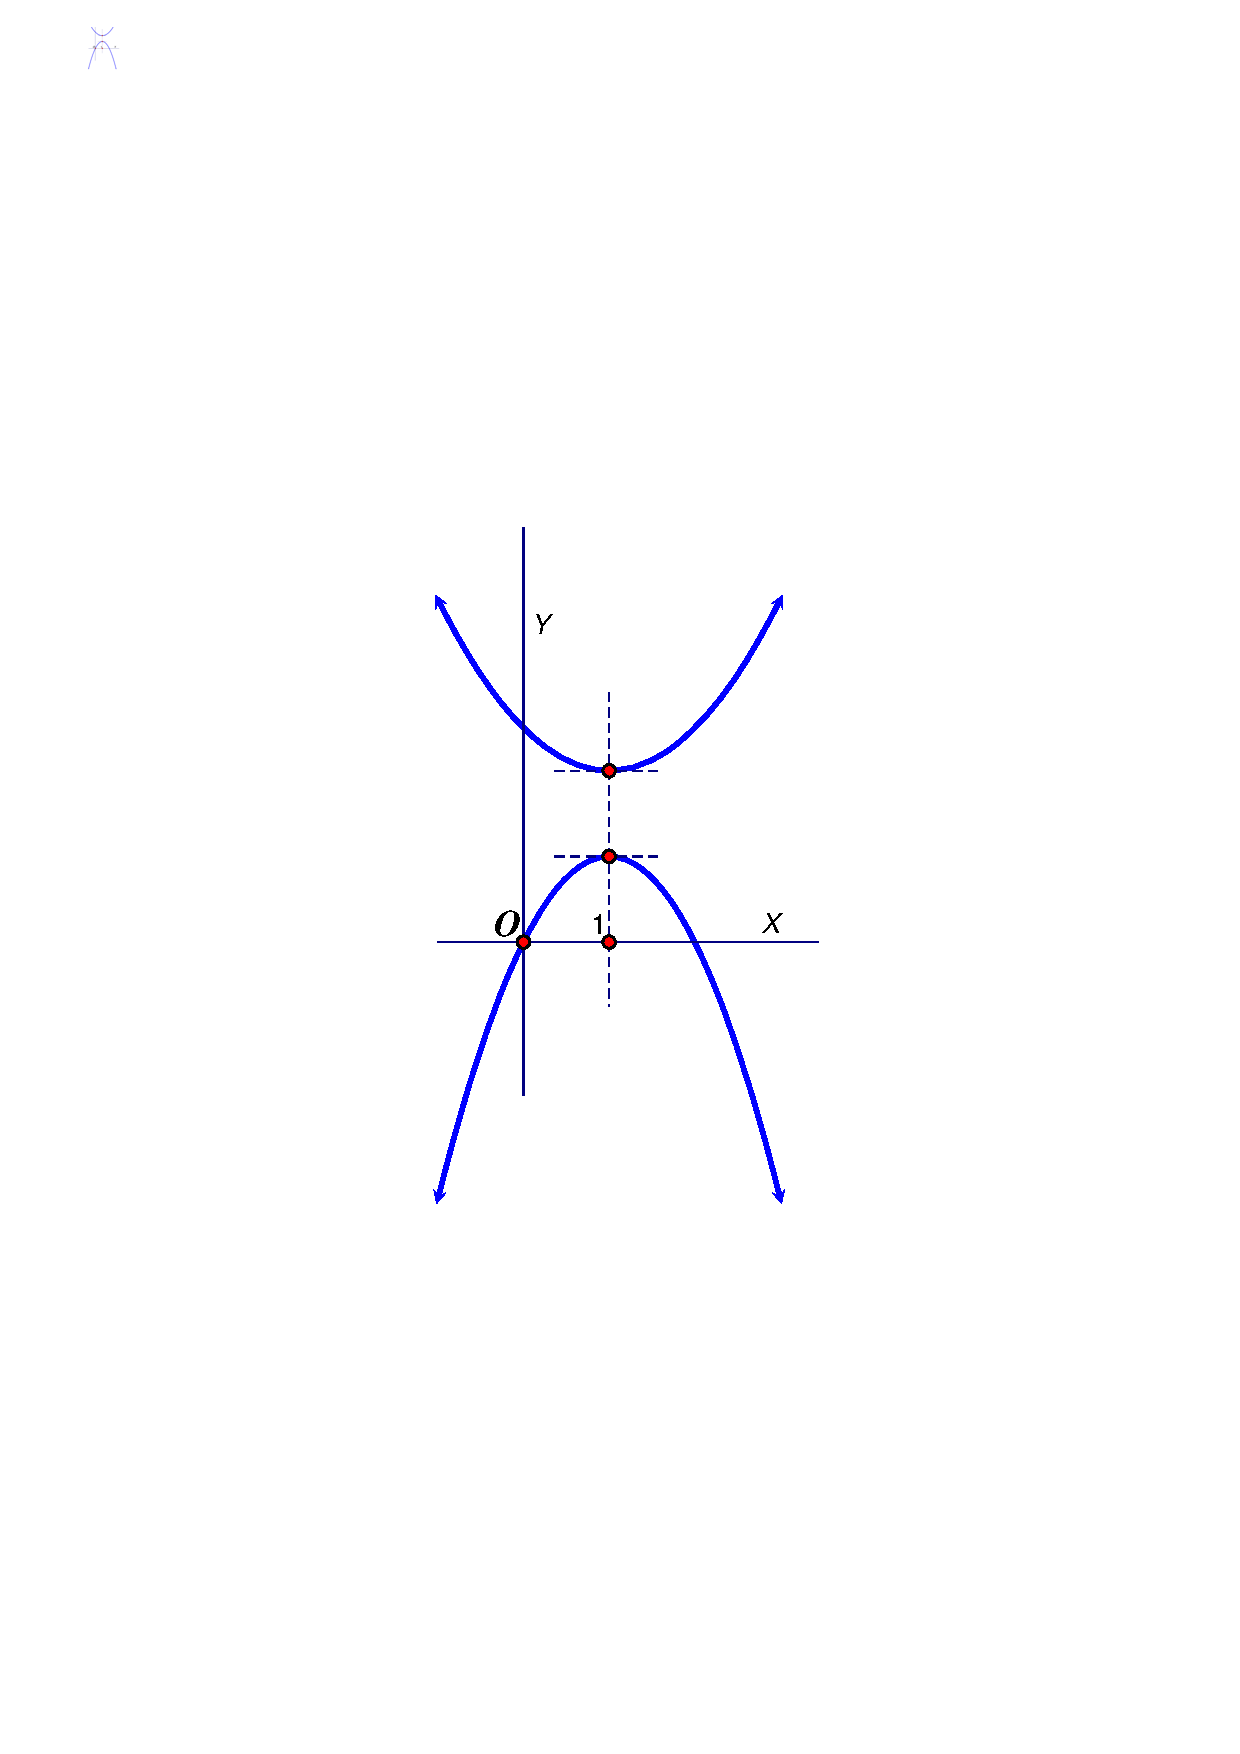
\includegraphics[trim=3cm 10cm 3cm
 10.3cm,width=0.55\textwidth,clip]{kernen.pdf}
  \\Figur 8.7: To vektorer i kernen 
\end{center}

\textbf{Bestemmelse af kernen}:\\
Idet $\,P'(x)=2ax+b\,$ får vi at $P(x)\in \ker(f)$ hvis og kun hvis
$$P'(1)=2a+b=0\,,$$
det vil sig hvis og kun hvis
$$b=-2a\,.$$
Et andengradspolynomium tilhører derfor kernen for $f\,$ hvis og kun hvis det har forskriften
$$P(x)=ax^2-2ax+c=a\cdot(x^2-2x)+c\cdot 1\,.$$
Vi ser at kernen er udspændt af de to lineært uafhængige polynomier $\,(x^2-2x)\,$ og $\,1\,$, og konkluderer at  $(\,x^2-2x\,,\,1\,)\,$ er en basis for kernen. Hermed er $\ker(f)$ bestemt.\bs

\textbf{Bestemmelse af billedrummet}:\\
For ethvert $k\in\mathbb R$ findes der andengradspolynomier $P(x)$ som opfylder $\,P'(1)=k\,$. Det gør for eksempel $\,P(x)=0x^2+kx+0=kx\,$. Vi konkluderer at billerummet $\,f\big(\,P_2(\mathbb R)\,\big)=\mathbb R\,.$
\end{example}

\section{Afbildningsmatrix}
Alle lineære afbildninger fra et endeligt dimensionalt definitionsrum $V$ til et endeligt dispositionsrum $W$ lader sig beskrive ved hjælp af en \textit{afbildningsmatrix}. Det handler dette afsnit om. Forudsætningen er blot at der vælges en basis for både $V$ og $W$, og at vi overgår fra vektorregning til regning med vektorernes koordinater med hensyn til de valgte baser. Den store fordel ved dette setup er at vi kan opstille generelle regnemetoder for alle lineære afbildninger mellem endeligt-dimensionale vektorrum. Det ser vi på senere afsnit, se afsnit \ref{tn8.secBrugAfbildnM}. Her drejer det sig hvordan man opstiller afbildningsmatricerne.\bs 
Vi begynder med at betragte en afbildning $\,f:\mathbb R^n\rightarrow \mathbb R^m\,$ som har form af et matrix-vektorprodukt:
\begin{equation}\label{tn8.afbMatrix1}
\mathbf y = f(\mathbf x)=\mA\,\mathbf x\,.
\end{equation}
Da det fremgår at $\mathbf x \in \reel^n$ og $\mathbf y \in  \reel^m$ giver forskriften \eqref{tn8.afbMatrix1} mening netop når $\mA$ er en $m\times n-$matrix. Ved at benytte  regneregler for matrixprodukt, se \tref{NUID2-tn3.regneregler2}{sætning}, opnår vi for ethvert valg af $\mathbf x_1\,,\mathbf x_2\in \reel^n$ og enhver skalar $k$:
$$f(\mathbf x_1+\mathbf x_2)=\mA\,(\mathbf x_1+\mathbf x_2)=
\mA\mathbf x_1+\mA\mathbf x_2=f(\mathbf x_1)+f(\mathbf x_2)\,,$$
$$f(k\mathbf x_1)=\mA\,(k\mathbf x_1)=k(\mA\,\mathbf x_1)=kf(\mathbf x_1)\,.$$
Vi ser at afbildningen opfylder linearitetsbetingelserne $L_1$ og $L_2\,$. Enhver afbildning af formen (\ref{tn8.afbMatrix1}) er derfor lineær.
\begin{example}[Afbildning ved hjælp af matrix]
Formlen:
$$\begin{matr}{r}y_1\\y_2\\y_3\end{matr}
=\begin{matr}{rr}1&2\\3&4\\5&6\end{matr}\,
\begin{matr}{r}x_1\\x_2\end{matr}
=\begin{matr}{r}x_1+2x_2\\3x_1+4x_2\\5x_1+6x_2\end{matr}$$
angiver en lineær afbildning fra vektorrummet $\mathbb R^2$ til vektorrummet $\mathbb R^3\,.$
\end{example}

Men også det modsatte gælder: Enhver lineær afbildning mellem endeligt-dimensionale vektorrum kan skrives som et matrix-vektorprodukt på formen (\ref{tn8.afbMatrix1}) hvis vi erstatter $\mathbf x$ og $\mathbf y$ med deres koordinatar med hensyn til en valgt basis i definitionsrummet henholdsvis dispositionsrummet. Dette viser vi i det følgende.\\

Vi betragter nu en lineær afbildning $\,f:V\rightarrow W\,$ hvor $V$ er et n-dimensionalt og $W$ et m-dimensionalt vektorrum, se figur 8.8:
\begin{center}
		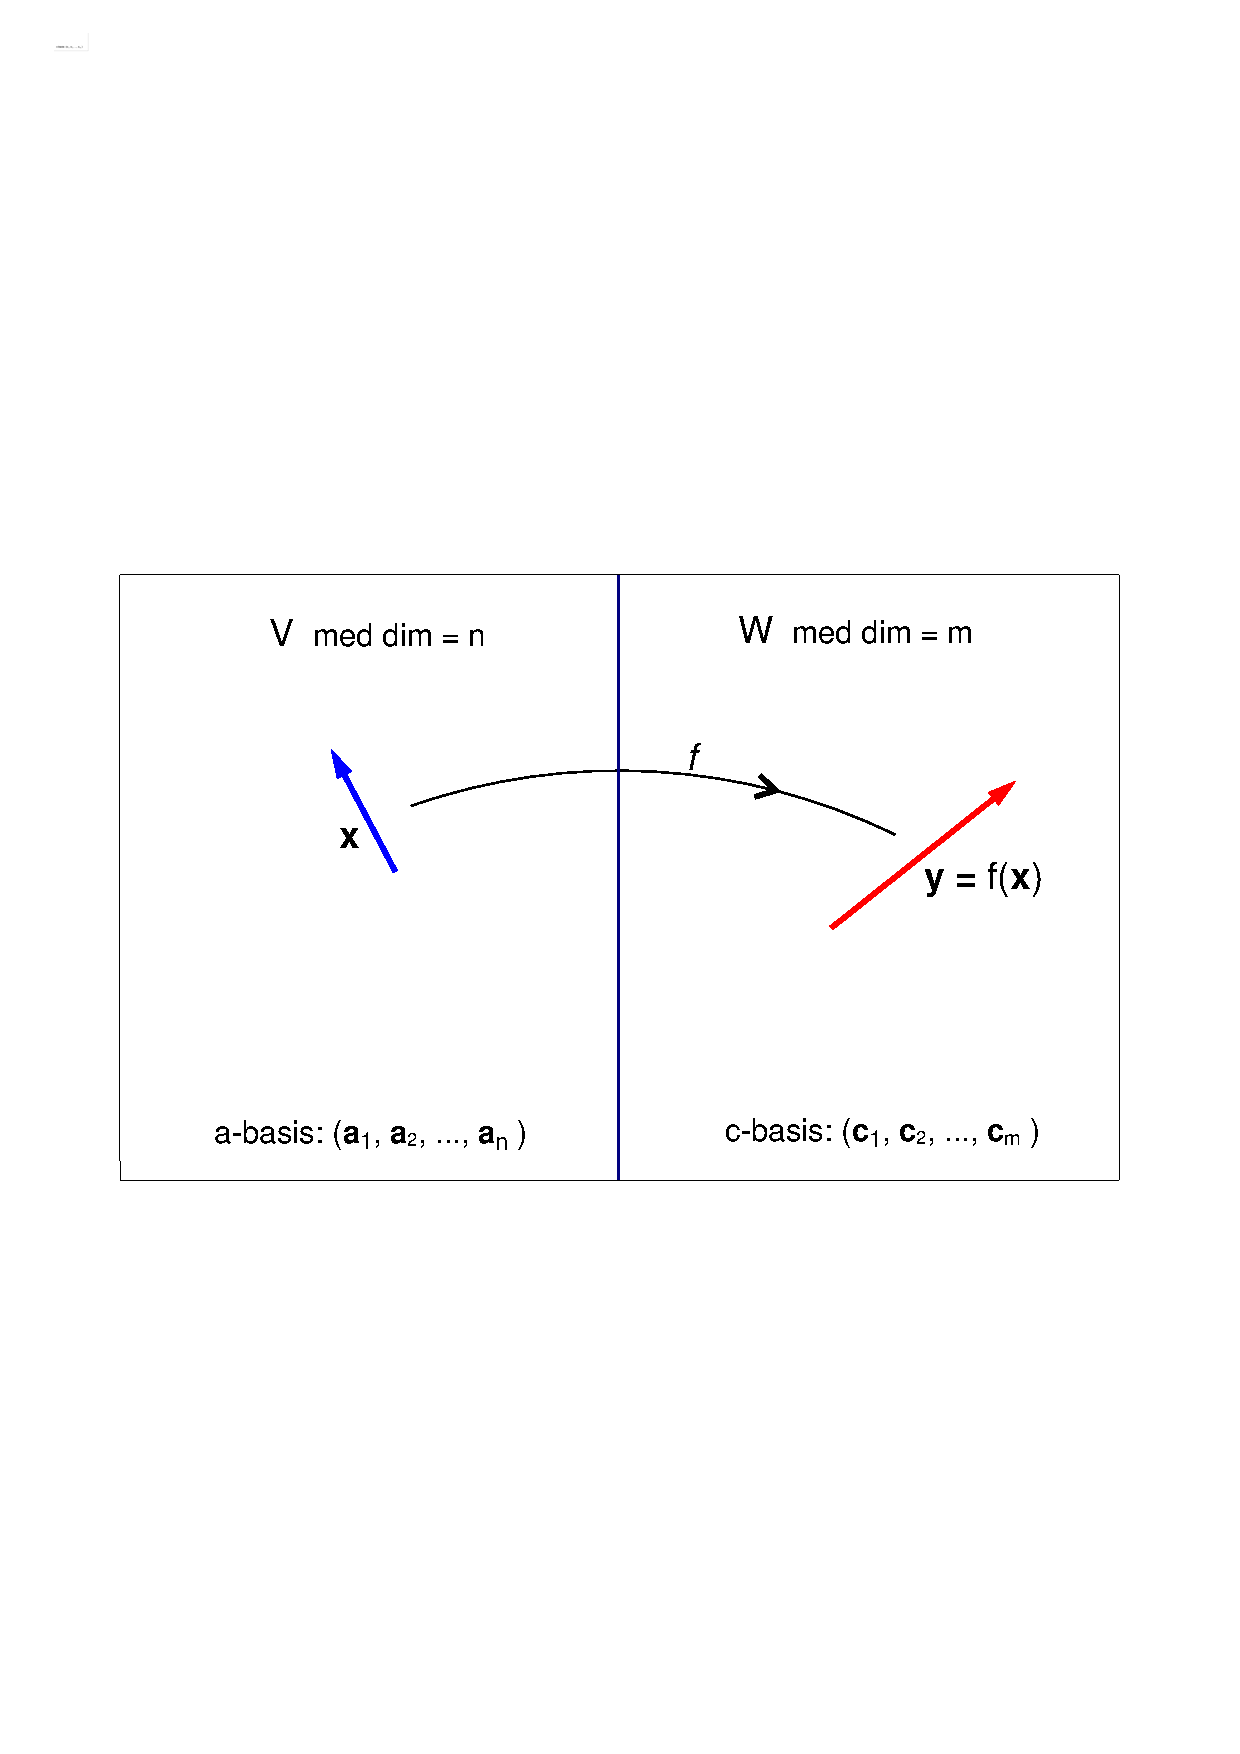
\includegraphics[trim=2cm 9cm 2cm
 9cm,width=0.60\textwidth,clip]{linAfbVW.pdf}
  \\Figur 8.8: Lineær afbildning 
\end{center}

For $V$ er der valgt en basis $a$ og for $W$ en basis $c$. Det betyder at en given vektor $\mathbf x \in V$ kan skrives som  en unik linearkombination af $a$-basisvektorerne, og at billedet $\mathbf y = f(\mathbf x)$ kan skrives som  en unik linearkombination af $c$-basisvektorerne:
$$\mathbf x=x_1\ma_1+x_2\ma_2+\ldots+x_n\ma_n\,\,\,\mathrm{og}\,\,\,
\mathbf y=y_1\mc_1+y_2\mc_2+\cdots+y_m\mc_m\,.$$
Det betyder at $(x_1,x_2,\ldots,x_n)$ er koordinatsæt for $\mathbf x$ med hensyn til $a$-basis, og at $(y_1,y_2,\ldots,y_m)$ er koordinatsæt for $\mathbf y$ med hensyn til $c$-basis.\\

Vi stiller nu spørgsmålet: Hvordan kan vi beskrive relationen mellem $a$-koordinatvektoren for vektor $\mathbf x \in V$ og $c$-koordinatvektoren for billedvektoren $\mathbf y$? Vi er med andre ord på jagt efter relationen mellem:

$$\vekind cy=\begin{matr}{r}y_1\\y_2\\ \vdots \\y_m\end{matr}\mathrm{\,\,\,og\,\,\,}
\vekind ax=\begin{matr}{r}x_1\\x_2\\ \vdots \\x_n\end{matr}\,.$$
Dette udvikler vi gennem de følgende omskrivninger hvor vi først, ved hjælp af $L_1$ og $L_2$, får opskrevet $\mathbf y$ som en linearkombination af billederne af $a$-vektorerne.
\begin{align*}
\mathbf y&=f(\mathbf x)\\
&=f(x_1\ma_1+x_2\ma_2+\cdots+x_n\ma_n)\\
&=x_1f(\ma_1)+x_2f(\ma_2)+\cdots+x_nf(\ma_n)\,.
\end{align*}
Herefter kan vi undersøge koordinatvektoreren for $\mathbf y$ med hensyn til $c$-basis, idet vi først bruger koordinatsætningen, se \tref{NUID18-tn7.koord_linearitet}{sætning}, og derefter definitionen på matrixvektor-produkt, se \tref{NUID2-tn3.prodvektor}{definition}.
\begin{align*}
\vekind cy&=\, _\mathrm c\big(\,x_1f(\ma_1)+x_2f(\ma_2)+\cdots+x_nf(\ma_n)\,\big)\\
&=x_1\,_\mathrm cf(\ma_1)+x_2\,_\mathrm cf(\ma_2)+\cdots+x_n\,_\mathrm cf(\ma_n)\\
&=\begin{matr}{rrrr}
_\mathrm cf(\ma_1)& _\mathrm cf(\ma_2)&\cdots&_\mathrm cf(\ma_n)\end{matr}\,\vekind ax\,.
\end{align*}

Matricen $\,\begin{matr}{rrrr}
_\mathrm cf(\ma_1)& _\mathrm cf(\ma_2)&\cdots&_\mathrm cf(\ma_n)\end{matr}\,$ i den sidste ligning kaldes \textit{afbildningsmatricen} for $f$ med hensyn til $a$-basis i $V$ og $c$-basis  i $W$.\\

Vi har hermed opnået dette vigtige resultat: Koordinatvektoren $\vekind cy$ kan opnås ved at man ganger afbildningsmatricen med koordinatvektoren $\vekind ax$. Resultaterne opsummerer vi nu i det følgende.

\begin{definition}[Afbildningsmatrix]\label{tn8.DefAfbMatrix}
Lad $f:V\rightarrow W$ være en lineær afbildning fra et $n$-dimensionalt vektorrum $ V $ til et $m$-dimensionalt vektorrum $W\,$. Ved \ind{afbildningsmatrix}{afbildningsmatricen} for $f$ med hensyn til basis $\,a\,$ i $V$ og basis $\,c\,$ i $W$ forstås $m\times n$-matricen:
\begin{equation}
\matind cFa = \begin{matr}{rrrr}
_\mathrm cf(\ma_1)& _\mathrm cf(\ma_2)&\cdots&_\mathrm cf(\ma_n)\end{matr}\,.
\end{equation}
Afbildningsmatricen for $f$ består dermed af de $n$ $c$-koordinatvektorer for billederne ved $f$ af de $n$ $a$-basisvektorer i $V\,$.
\end{definition}

Hovedopgaven for en afbildningsmatrix er naturligvis at kunne bestemme billeder i $W$ af vektorer i $V$, og den legitimeres af den følgende sætning som er en opsummering af undersøgelserne ovenfor.

\begin{theorem}[Hovedsætning om afbildningsmatrix]\label{tn8.ThAfbMatrix}
Lad $ V $ være et $n$-dimensionalt vektorrum med valgt basis $a$ og $ W $ et $m$-dimensionalt vektorrum med valgt basis $c\,.$ 
\begin{enumerate}
\item 
For en lineær afbildning $f:V\rightarrow W$ gælder at hvis $\,\mathbf y=f(\mathbf x)\,$ er billedet af en vilkårlig vektor $\,\mathbf x \in V\,,$ så gælder der:
\begin{equation}
\vekind cy=\matind cFa\,\vekind ax\, 
\end{equation}
hvor $\matind cFa$ er afbildningsmatricen for $f$ hensyn til basis $\,a\,$ i $V$ og basis $\,c\,$ i $W\,.$
\item
Antag omvendt at billederne $\,\mathbf y=g(\mathbf x)\,$ for en afbildning $g:V\rightarrow W$ kan fås på koordinatform ved
\begin{equation}
\vekind cy=\matind cGa\,\vekind ax\,
\end{equation}
hvor $\,\matind cGa \in \reel^{m\times n}\,,$ så er $g$ lineær, og $\matind cGa$ er afbildningsmatricen for $g$ hensyn til basis $\,a\,$ i $V$ og basis $\,c\,$ i $W\,.$.
\end{enumerate}
\end{theorem}

Herefter følger tre eksempler på opstilling og elementær brug af afbildningsmatricer. 

\begin{example}[Opstilling og brug af afbildningsmatrix] \label{tn8.brugAfbM3}
Drejning af plane vektorer afsat ud fra Origo er et enkelt eksempel på en lineær afbildning, se opgave \ref{tn8.opgDrejning}. Lad $v$ være en vilkårlig vinkel, og lad $f$ være den lineære afbildning der drejer en vilkårlig vektor vinkel $v$ omkring Origo mod uret, se figur 8.9.
\begin{center}
		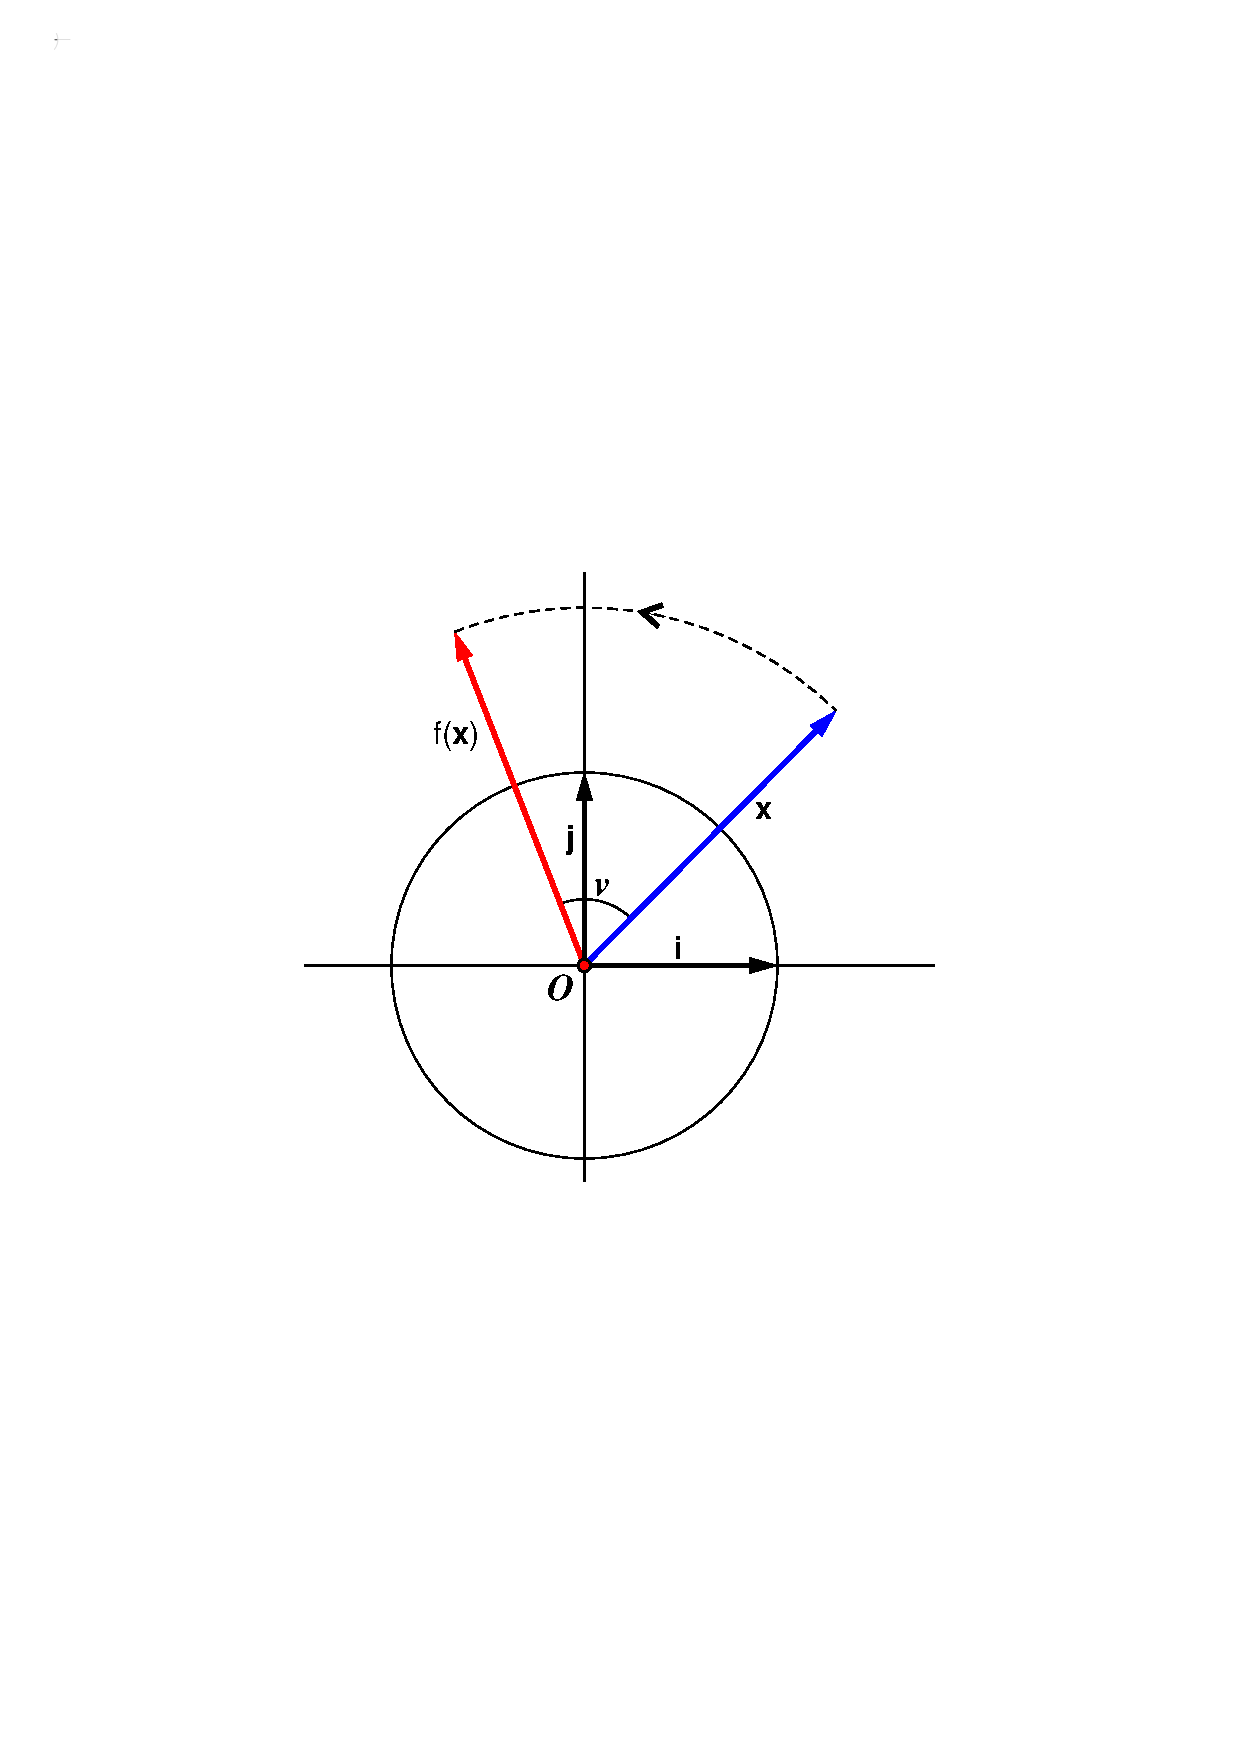
\includegraphics[trim=2cm 9cm 2cm
 9cm,width=0.60\textwidth,clip]{drejning.pdf}
  \\Figur 8.9: Lineær drejning omkring Origo 
\end{center}

Vi ønsker at bestemme afbildningsmatricen for $f$ med hensyn til standardbasen for vektorer i planen. Vi har derfor brug for billederne af basisvektorerne $\mathbf i$ og $\mathbf j\,$, se figur 8.10.
\begin{center}
		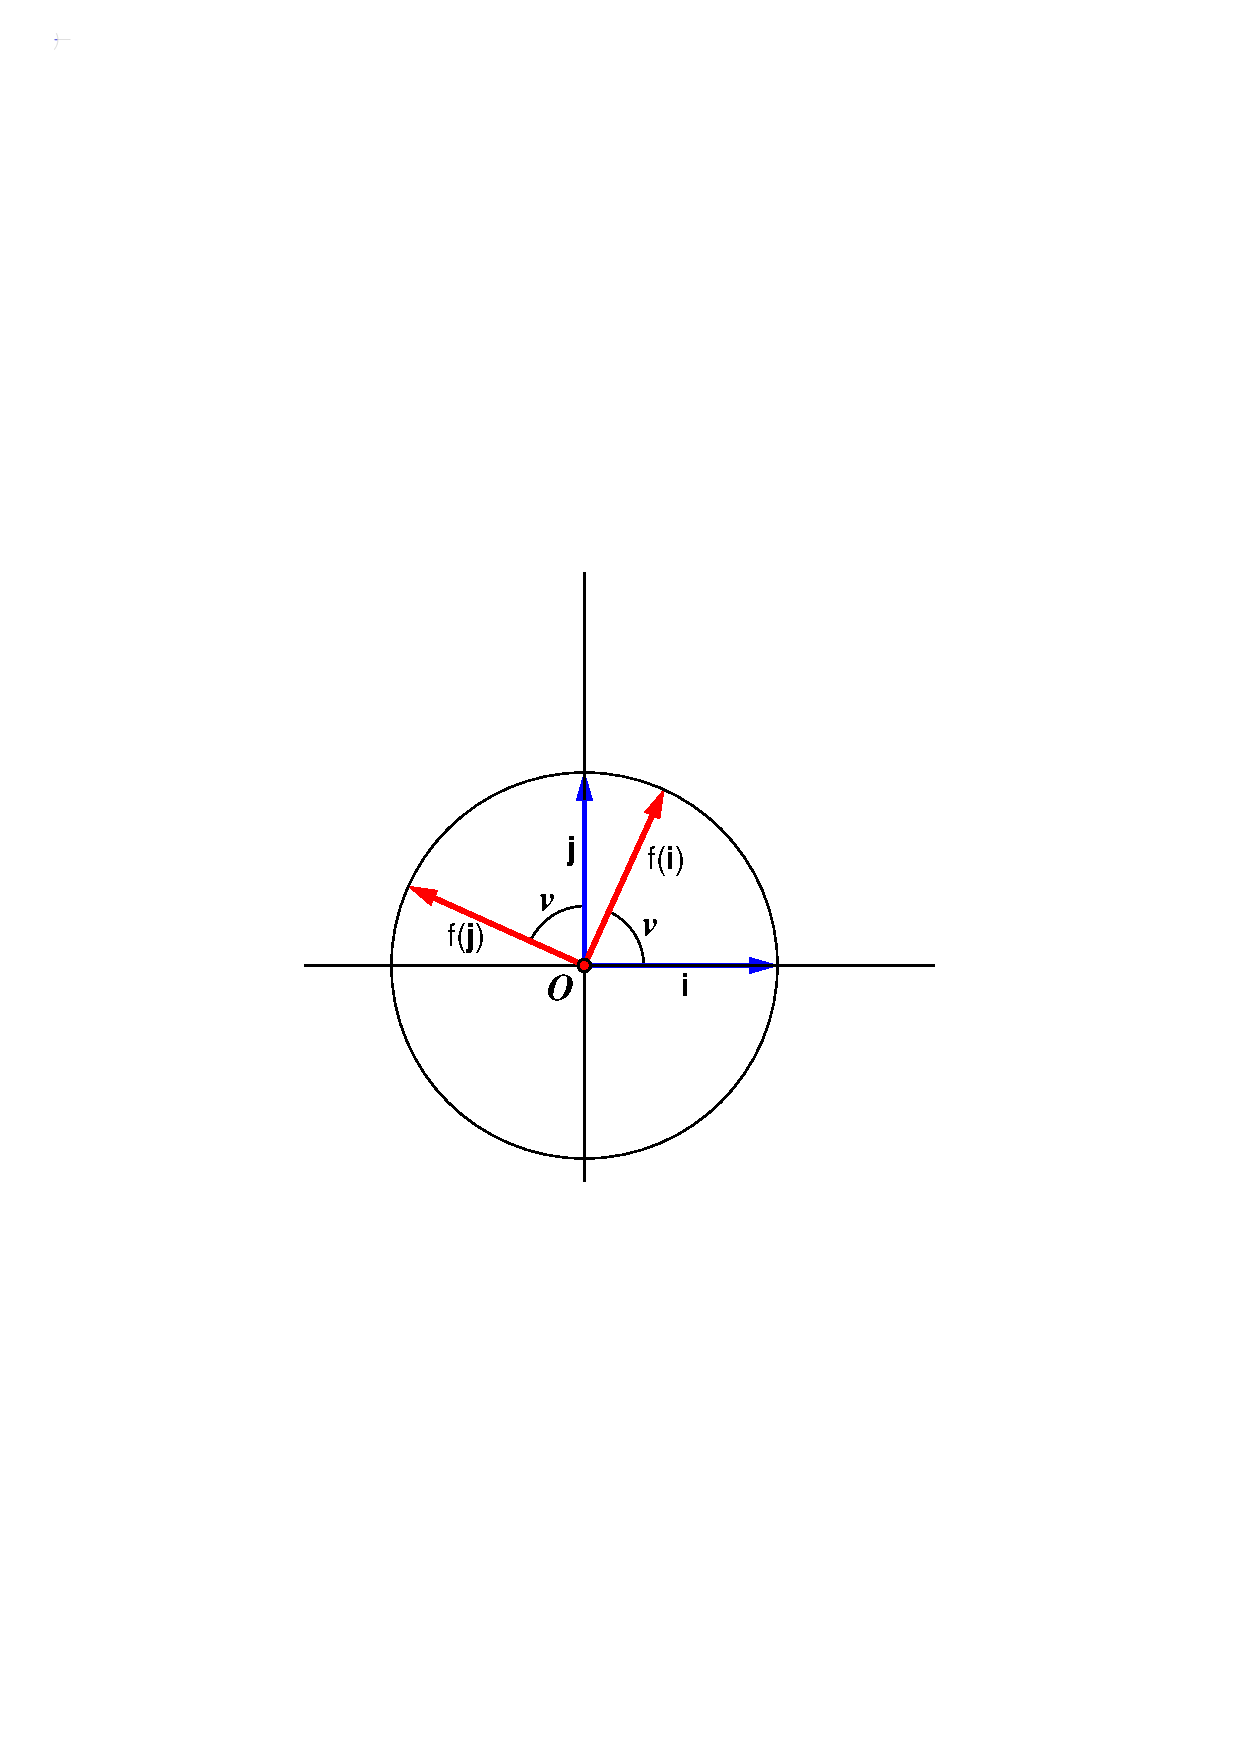
\includegraphics[trim=2cm 9cm 2cm
 12cm,width=0.60\textwidth,clip]{drejning2.pdf}
  \\Figur 8.10: Bestemmelse af afbildningsmatrix 
\end{center}
Det ses at $ f(\mathbf i)=\left(\cos(v),\sin(v)\right) $ og $ f(\mathbf j)=\left(-\sin(v),\cos(v)\right)$. Den ønskede afbildningsmatrix er derfor
$$\matind eFe=\begin{matr}{rr}\cos(v)&-\sin(v)\\\sin(v)&\cos(v)\end{matr}\,.$$
Koordinaterne for billedet $\,\mathbf y=f(\mathbf x)\,$ af en given vektor $\mathbf x$ fås dermed ud fra ligningen:
$$
\begin{matr}{r}y_1\\y_2\end{matr}=
\begin{matr}{rr}\cos(v)&-\sin(v)\\\sin(v)&\cos(v)\end{matr}
\,\begin{matr}{r}x_1\\x_2\end{matr}\,.
$$
\end{example}

\begin{example}[Opstilling og brug af afbildningsmatrix] \label{tn8.brugAfbM1}
I et 3-dimensionalt vektorrum $V$ er der valgt en basis $(\ma_1,\ma_2,\ma_3)\,$, og i et 2-dimensionalt vektorrum $W$ er der valgt en basis $(\mc_1,\mc_2)\,$. En lineær afbildning $\,f:V\rightarrow W\,$ opfylder at:
\begin{equation}\label{tn8.exAfbM2}
f(\ma_1)=3\mc_1+\mc_2\,,\,\,f(\ma_2)=6\mc_1-2\mc_2\,\,\,\mathrm{og}\,\,\,f(\ma_3)=-3\mc_1+\mc_2\,.
\end{equation}
Vi ønsker at finde billedet ved $f$ af vektoren $\mv=\ma_1+2\ma_2+\ma_3\in V\,$ ved hjælp af afbildningsmatricen $\matind cFa\,$. Afbildningsmatricen opstilles nemt da vi allerede fra (\ref{tn8.exAfbM2}) kender billederne af basisvektorerne i $V\,$:
\begin{equation*}
\matind cFa = \begin{matr}{rrr}
_\mathrm cf(\ma_1)& _\mathrm cf(\ma_2)&_\mathrm cf(\ma_3)\end{matr}\,
=\begin{matr}{rrr}
3&6&-3\\
1&-2&1\end{matr}
\end{equation*}
Da $\mv$ har koordinatsættet $(1,2,1)$ med hensyn til $a$-basis, finder vi koordinatvektoren for $f(\mv)$ således:
$$_\mathrm cf(\mv)= \matind cFa \, \vekind av = \begin{matr}{rrr}
3&6&-3\\
1&-2&1\end{matr}\,\begin{matr}{r}1\\2\\1\end{matr}
=\begin{matr}{r}12\\-2\end{matr}\,.
$$
Vi har hermed fundet $\,f(\mv)=12\mc_1-2\mc_2\,$.
\end{example}

\begin{example}[Opstilling og brug af afbildningsmatrix] \label{tn8.brugAfbM2}
En lineær afbildning $f: \mathbb R^4\rightarrow \mathbb R^3$ er givet ved:
\begin{equation}\label{tn8.exAfbM1}
f(x_1,x_2,x_3,x_4)
=\begin{matr}{c}
x_1+2x_2+x_4\\
2x_1-x_2+2x_3-x_4\\
x_1-3x_2+ 2x_3-2x_4
\end{matr}\,.
\end{equation}
Lad os bestemme afbildningsmatricen for $f$ med hensyn til standard e-basis i $\mathbb R^4$ og standard e-basis i $\mathbb R^3\,$. Først finder vi billederne af de fire $e$-basisvektorer i $\mathbb R^4$ ved hjælp af forskriften (\ref{tn8.exAfbM1}):
$$
f(1,0,0,0)=
 \begin{matr}{r}1\\2\\1\end{matr}\,,\,\,\,
f(0,1,0,0)= 
 \begin{matr}{r}2\\-1\\-3\end{matr}\,,$$
$$f(0,0,1,0)= 
  \begin{matr}{r}0\\2\\2\end{matr}\,,\,\,\,
f(0,0,0,1)=  
 \begin{matr}{r}1\\-1\\-2\end{matr}\,.
$$
Vi kan nu opstille afbildningsmatricen for $f$:
\begin{equation}
\matind eFe = \begin{matr}{rrrr}
1&2&0&1\\
2&-1&2&-1\\
1&-3&2&-2\end{matr}\,.
\end{equation}
Vi ønsker at finde billedet $\mathbf y=f(\mathbf x)$ af vektoren $\mathbf x=(1,1,1,1)$. Til rådighed har vi naturligvis forskriften (\ref{tn8.exAfbM1}), men vi vælger at finde billedet ved hjælp af afbildningsmatricen:

$$
\vekind ey=\matind eFe\,\vekind ex
=\begin{matr}{rrrr}
1&2&0&1\\
2&-1&2&-1\\
1&-3&2&-2\end{matr}\,
\begin{matr}{r}1\\1\\1\\1\end{matr}=
\begin{matr}{r}4\\2\\-2\end{matr}\,.
$$
Vi har hermed fundet $\vekind ey= {_\mathrm e f}(1,1,1,1)=(4,2,-2)\,$.
\end{example}

\begin{exercise}\label{tn8.spejlingsopg2}
I planen er der givet et sædvanligt $\,(O,\mathbf i,\mathbf j)$-koordinatsystem, og alle vektorer tænkes afsat ud fra Origo. Spejling af vektorer i linjen $\,y=\frac 12 x\,$ er en lineær afbildning, lad os kalde den $s\,$.\\

Bestem $s(\mathbf i)$ og $s(\mathbf j)$, opstil afbildningsmatricen $\matind eSe$ for $s\,$ og bestem et udtryk for spejlingen af en vilkårlig plan vektor $\,\mathbf v\,$ med $e$-koordinaterne $(v_1,v_2)\,$. Figur 8.11 indholder nogle hints til bestemmelse af $s(\mathbf i)$. Gå frem på tilsvarende vis med $s(\mathbf j)\,$.

\begin{center}
		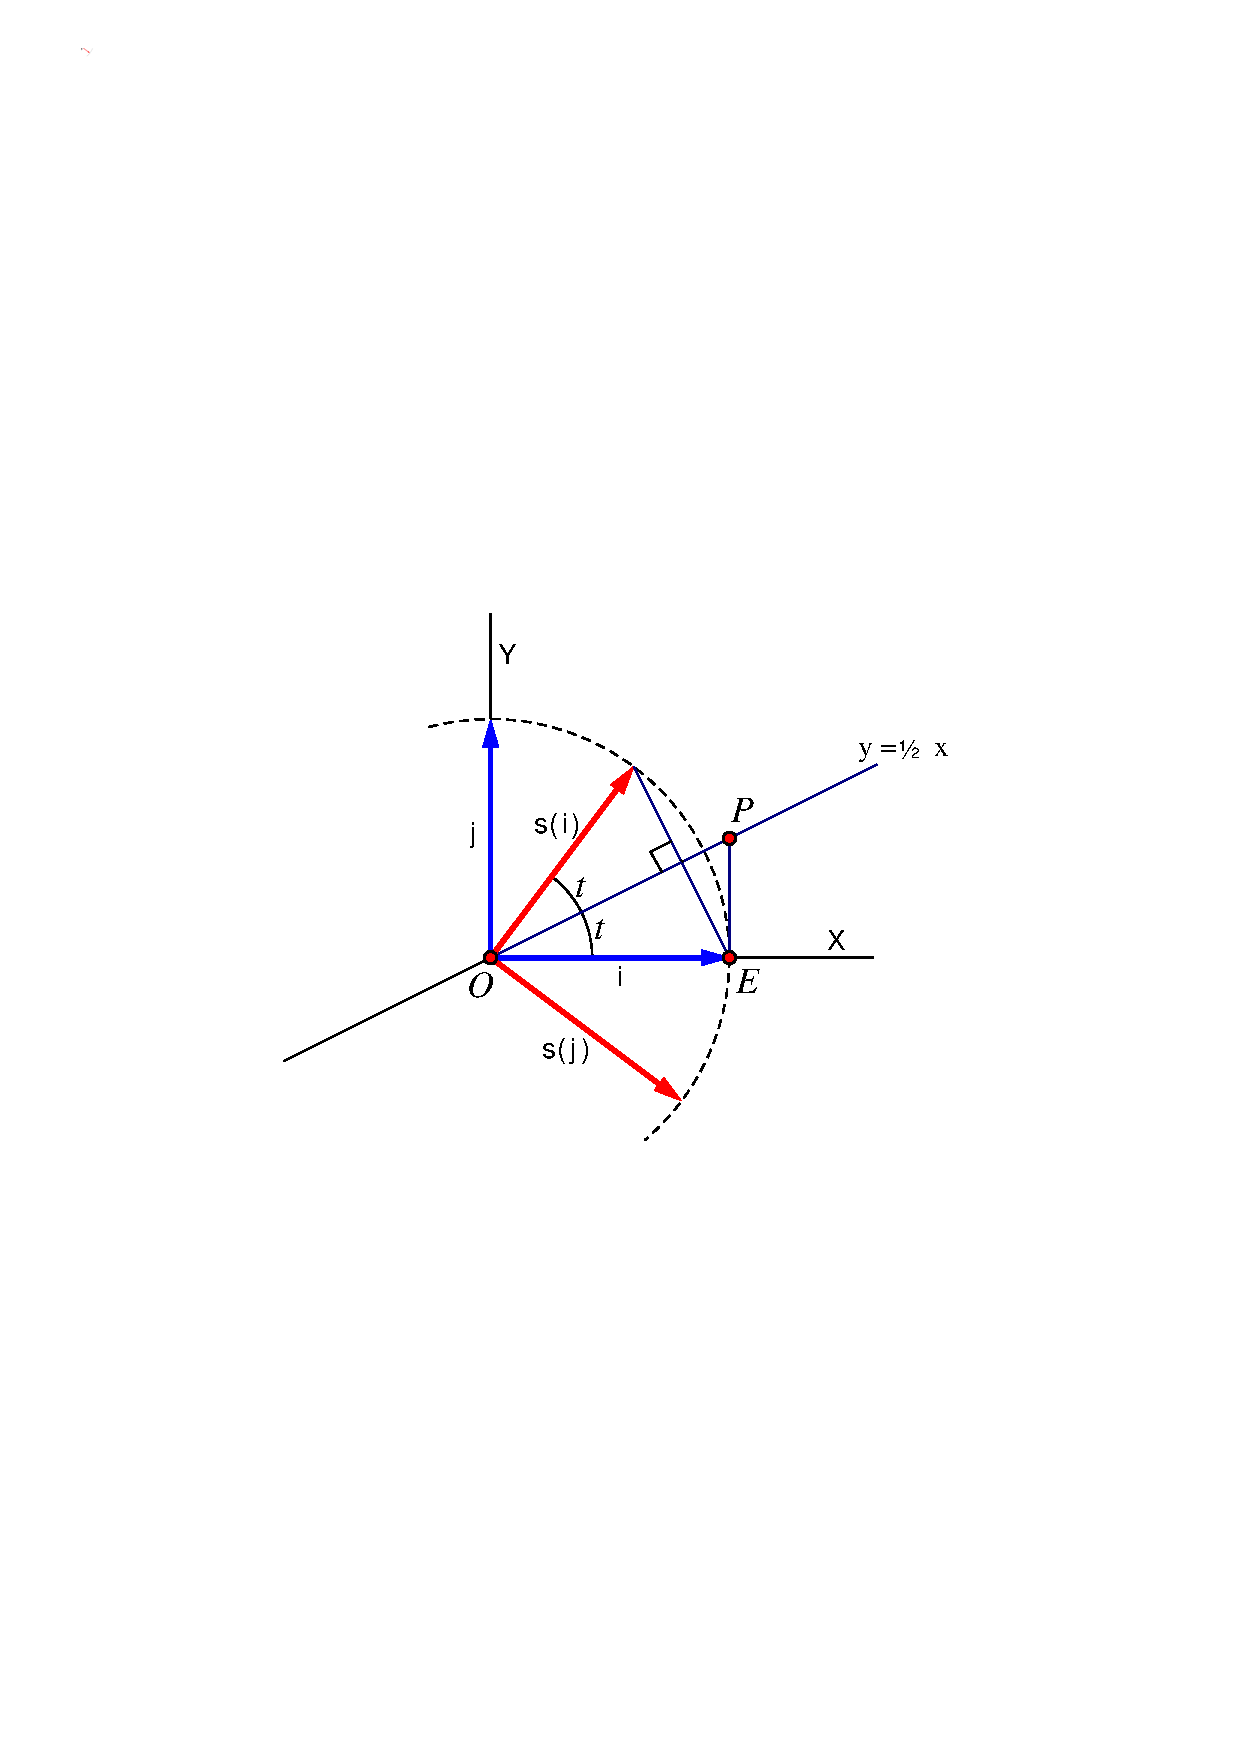
\includegraphics[trim=2cm 9cm 2cm
 12cm,width=0.60\textwidth,clip]{spejling2.pdf}
  \\Figur 8.11: Spejling af standardbasisvektorer.
\end{center}
\end{exercise}

\section{Om brug af afbildningsmatricer}\label{tn8.secBrugAfbildnM}

Afbildningsmatricer er et meget perspektivrigt redskab. Det tillader os at oversætte spørgsmål om lineære afbildninger mellem vektorrum til spørgsmål om matricer og koordinatvektorer som vi umiddelbart kan regne på. Metoderne forudsætter blot at der er valgt en basis i hvert af vektorrummene, og at den afbildningsmatrix som hører til de to baser, er opstillet. Sådan kan vi reducere spørgsmål af så forskellig karakter som at finde polynomier med visse egenskaber, at finde resultatet af en geometrisk konstruktion og at løse differentialligninger, til spørgsmål der kan undersøges ved hjælp af matrixalgebra.\bs

Som gennemgående eksempel ser vi på en lineær afbildning $\,f:V \rightarrow W\,$ hvor $V$ er et 4-dimensionalt vektorrum med  valgt basis $(\ma_1,\ma_2,\ma_3,\ma_4)$, og hvor $W$ er et 3-dimensionalt vektorrum med valgt basis $(\mc_1,\mc_2,\mc_3)\,$. Afbildningsmatricen for $f$ er:
\begin{equation}\label{tn8.exBrugAfbM}
\matind cFa=
\begin{matr}{rrrr}
1&3&-1&8\\
2&0&4&-2\\
1&-1&3&-4\end{matr}\,.
\end{equation}

\subsection{At finde kernen for \textit{f}}

Når man skal finde kernen for $f$, skal man finde alle $\mathbf x\in V$ som afbildes i $\mnul\in W$. Det vil sige at man skal løse vektorligningen 
$$
 f(\mathbf x)=\mnul\,.
$$
Denne ligning er ifølge sætning \ref{tn8.ThAfbMatrix} ensbetydende med matrixligningen  
$$
\matind cFa\,\vekind ax = \vekind c\mnul$$
$$\,\Leftrightarrow\,
\begin{matr}{rrrr}
1&3&-1&8\\
2&0&4&-2\\
1&-1&3&-4\end{matr}
\begin{matr}{r}x_1\\x_2\\x_3\\x_4\\\end{matr}
=\begin{matr}{r}0\\0\\0\\\end{matr}
$$
som svarer til et homogene lineære ligningssystem med totalmatricen:
$$
\mT=
\begin{matr}{rrrr|r}
1&3&-1&8&0\\
2&0&4&-2&0\\
1&-1&3&-4&0\end{matr}\,
\rightarrow \mathrm{trap}(\mT)=
\begin{matr}{rrrr|r}
1&0&2&-1&0\\
0&1&-1&3&0\\
0&0&0&0&0\end{matr}\,.
$$
Det ses at løsningsmængden er udspændt af to lineært uafhængige vektorer: $(-2,1,1,0)$ og $(1,-3,0,1)$. Lad  $\mathbf v_1$ og $\mathbf v_2$ være de to vektorer i $V$, som er bestemt ved $a$-koordinater således:
$$\vekind av_1=(-2,1,1,0)\mathrm{\;\;og\;\;}\vekind av_2=(1,-3,0,1)\,.$$
Så er $(\mathbf v_1,\mathbf v_2)$ en basis for kernen for $f$, og kernen for $f$ har dimensionen 2.\bs
\textit{Pointe}: Antallet $n=4$ af ubekendte i det løste ligningssystem er pr. definition lig med antallet af søjler i $\matind cFa\,$ som igen er lig med $ \dim(V) $, se definition \ref{tn8.DefAfbMatrix}. Endvidere bemærkes at ligningssystemets koefficientmatrix er identisk med $\matind cFa\,$. Hvis rangen af koefficientmatricen er $k\,$, ved vi at løsningsmængden og dermed kernen er udspændt af $(n-k)$ lineært uafhængige retningsvektorer hvor $k$ er rangen af koefficientmatricen. Derfor har vi:
$$\dim(\mathrm{kernen})=n-\rho\,(\matind cFa)=4-2=2\,.$$

\begin{method}[Bestemmelse af kernen]\label{tn8.metodeKerne}
I et vektorrum $V$ er der valgt en basis $a$, og i et vektorrum $ W $ er der valgt en basis $c$. Kernen for en lineær afbildning $\,f:V\rightarrow W,$ kan i koordinatform findes som løsningsmængden for det homogene lineære ligningssystem som har totalmatricen
$$\mT=
\begin{matr}{r|r}\matind cFa & \vekind c\mnul \end{matr}\,.$$
Kernen er et underrum i $V\,$, og dens dimension er bestemt ved:
\begin{equation}\label{tn8.methodKernen}
\mathrm{dim}(\,\ker(f)\,)=\mathrm{dim}(V)-\rho\,(\matind cFa)\,.
\end{equation}
\end{method}

\subsection{At løse vektorligningen \textit{f(x) = b}}
Hvordan kan man afgøre om en vektor $\mb \in W$ tilhører billedrummet for en given lineære afbildning. Spørgsmålet er om der findes (mindst) et $\mathbf x \in V$ som afbildes i $\mb\,,$ og det kan udvides til hvordan man kan bestemme alle $\mathbf x \in V$ med denne egenskab som afbildes i $\mb\,.$\bs
Vi betragter igen den lineære afbildning $\,f:V\rightarrow W\,$ der er repræsenteret af afbildningsmatricen (\ref{tn8.exBrugAfbM}), og vælger som eksempel den vektor $\mb \in W$ som har $c$-koordinaterne $(1,2,3)\,$. Vi skal løse vektorligningen 
$$f(\mathbf x)=\mb\,.$$
Regner vi i koordinater svarer vektorligningen til følgende matrixligning  
$$
\matind cFa\,\vekind ax = \vekind cb$$
det vil sige matrixligningen 
$$
\begin{matr}{rrrr}
1&3&-1&8\\
2&0&4&-2\\
1&-1&3&-4\end{matr}\,
\begin{matr}{r}x_1\\x_2\\x_3\\x_4\\\end{matr}
=\begin{matr}{r}1\\2\\3\\\end{matr}
$$
som svarer til et inhomogent lineært ligningssystem med totalmatricen:
$$
\mT=
\begin{matr}{rrrr|r}
1&3&-1&8&1\\
2&0&4&-2&2\\
1&-1&3&-4&3\end{matr}
$$
som ved GaussJordan-elimination reduceres til 
$$
\mathrm{trap}(\mT)=
\begin{matr}{rrrr|r}
1&0&2&-1&0\\
0&1&-1&3&0\\
0&0&0&0&1\end{matr}\,.
$$
Da rangen af totalmatricen her er større end rangen af koefficientmatricen, har det inhomogene ligningssystem ingen løsninger. Vi har altså fundet en vektor i $W$ som ingen ``originalvektor'' har i $V$. Bemærk at \textit{hvis} der havde været løsninger, så kunne den skrives op på strukturformen 
$\,L_{inhom} = \mathbf x_0 +L_{hom}\,$. Det vil i denne sammenhæng sige en partikulær løsning plus kernen for $f\,$.

\begin{method}[Løsning af vektorligningen \textit{f(x) = b}]\label{tn8.metodeVektorlign}
I et vektorrum $V$ er der valgt en basis $a$, og i et vektorrum $ W $ er der valgt en basis $c$. For en lineær afbildning $\,f:V\rightarrow W,$ og en egentlig vektor $\mb \in W$ kan ligningen
$$f(\mathbf x)=\mb$$
løses ved hjælp af det inhomogene lineære ligningssystem som har totalmatricen
$$\mT=
\begin{matr}{r|r}\matind cFa & \vekind cb \end{matr}\,$$
Hvis der findes løsninger, og $\mathbf x_0$ er én af disse løsninger, kan hele løsningsmængden opskrives som:
$$
\mathbf x_0+\ker(f)\,.$$
\end{method}

\subsection{At bestemme billedrummet}

Vi har ovenfor fundet at billedrummet for en lineær afbildning er et underrum i dispositionsrummet, se sætning \ref{tn8.thKernUrum}. Hvordan kan dette underrum afgrænses og karakteriseres? Det mest enkle og bekvemme er at finde en basis for underrummet!\bs
Vi betragter igen den lineære afbildning $\,f:V\rightarrow W\,$ der er repræsenteret af afbildningsmatricen (\ref{tn8.exBrugAfbM}). Da der er valgt basen $(\ma_1,\ma_2,\ma_3,\ma_4)$ for $ V $, kan vi opskrive samtlige vektorer i $V$ på én gang:
$$
\mathbf x=x_1\ma_1+x_2\ma_2+x_3\ma_3+x_4\ma_4\,,
$$
idet vi tænker os at $\,x_1,x_2,x_3\,$ og $\,x_4\,$ gennemløber alle tænkelige kombinationer af reelle værdier. Men så kan samtlige billeder i $W$ af vektorer i $V$ opskrives ved: 
%\begin{center}
\begin{align*}
f(\mathbf x)&=f(x_1\ma_1+x_2\ma_2+x_3\ma_3+x_4\ma_4)\\
&=x_1f(\ma_1)+x_2f(\ma_2)+x_3f(\ma_3)+x_4f(\ma_4)\,,
\end{align*}
%\end{center}
hvor vi har brugt $L_1$ og $L_2$, og hvor vi fortsat tænker os at $\,x_1,x_2,x_3\,$ og $\,x_4\,$ gennemløber alle tænkelige kombinationer af reelle værdier. Men så er:
$$f(V)=\mathrm{span}\left\{\,f(\ma_1),f(\ma_2),f(\ma_3),f(\ma_4)\,\right\}\,.$$
Billedrummet udspændes altså af $a$-basisvektorernes billeder! Men så kan vi efter ifølge \tref{NUID18-tn7.methodUdtynding}{metode} i eNote 7 bestemme en basis for billedrummet ved at finde de ledende 1-taller i trappeformen af 
$$\begin{matr}{rrrr}\vekind c f(\ma_1)&\vekind cf(\ma_2)&\vekind cf(\ma_3)&\vekind cf(\ma_4)\end{matr}\,.$$
Dette er jo afbildningsmatricen for $f$ med hensyn til de valgte baser
$$\matind cFa=
\begin{matr}{rrrr}
1&3&-1&8\\
2&0&4&-2\\
1&-1&3&-4\end{matr}
$$
som ved GaussJordan-elimination reduceres til
$$
\mathrm{trap}(\matind cFa)=
\begin{matr}{rrrr}
1&0&2&-1\\
0&1&-1&3\\
0&0&0&0\end{matr}\,.
$$
Til de to ledende 1-taller i $\,\mathrm{trap}(\matind cFa)\,$ svarer de to første søjler i $\,\matind cFa\,$. Vi konkluderer således:\bs
Lad  $\mathbf w_1$ og $\mathbf w_2$ være de to vektorer i W, som er bestemt ved $c$-koordinater således:
$$\vekind aw_1=(1,2,1)\mathrm{\;\;og\;\;}\vekind aw_2=(3,0,-1)\,.$$
Så er $(\mathbf w_1,\mathbf w_2)$ en basis for billedrummet $\,f(V)\,$.

\begin{method}[Bestemmelse af billedrummet]\label{tn8.metodeBilledrum}
I et vektorrum $V$ er der valgt en basis $a$, og i et vektorrum $W$ er der valgt en basis $c$. Billedrummet $\,f(V)\,$ for en lineær afbildning $\,f:V\rightarrow W,$ kan findes ud fra
\begin{equation}\label{tn8.methodBrum}
\mathrm{trap}(\matind cFa)
\end{equation}
på følgende måde: Hvis der i den $i$'te søjle i (\ref{tn8.methodBrum}) ikke er et ledende 1-tal, så fjernes $f(\ma_{\,i})$ fra vektorsættet $\,\big(\,f(\ma_1),f(\ma_2),\ldots,f(\ma_{\,n})\,\big)\,$. Når dette vektorsæt på denne måde er udtyndet, udgør det en basis for $\,f(V)\,$.\\

Da antallet af ledende 1-taller i (\ref{tn8.methodBrum}) er lig med antallet af basisvektorer i den valgte basis for $\,f(V)\,$, følger det at 
\begin{equation}\label{tn8.methodBrum2}
\mathrm{dim}(f(V))=\rho\,(\matind cFa)\,.
\end{equation}
\end{method}

\section{Dimensionssætningen}

I det foregående afsnits metode \ref{tn8.metodeKerne} fandt vi følgende udtryk for dimensionen af kernen for en lineær afbildning $\,f:V\rightarrow W\,$:
\begin{equation}\label{tn8.struktur1}
\mathrm{dim}(\,\ker(f)\,)=\mathrm{dim}(V)-\rho\,(\matind cFa)\,.
\end{equation}
Og i metode \ref{tn8.metodeBilledrum} et tilsvarende udtryk for billedrummet $f(V)\,$:
\begin{equation}\label{tn8.struktur2}
\mathrm{dim}(f(V)) = \rho\,(\matind cFa)\,.
\end{equation}
Ved at sammensætte (\ref{tn8.struktur1}) og (\ref{tn8.struktur2}) opnås en bemærkelsesværdig enkel sammenhæng mellem definitionsrummet, kernen og billedrummet for en lineær afbildning:

\begin{theorem}[Dimensionssætningen]\label{tn8.thDimension}
Lad $V$ og $W$ være to endeligt-dimensionale vektorrum. For en lineær afbildning $\,f:V\rightarrow W\,$ gælder:
$$
\mathrm{dim}(V)=\mathrm{dim}(\,\ker(f)\,)+
\mathrm{dim}\big(\,f(V)\,\big)\,.$$
\end{theorem}

Her er nogle umiddelbare konsekvenser af sætning \ref{tn8.thDimension}:
\begin{aha}
Billedrummet for en lineær afbildning kan aldrig have højere dimension end definitionsrummet.
\end{aha}
\begin{aha}
Hvis kernen kun indeholder $\mnul$-vektoren, bevarer billedrummet definitionsrummets dimension.
\end{aha}
\begin{aha} Hvis kernen har dimensionen $p>0$, så ``forsvinder'' der gennem afbildningen $p$ dimensioner. 
\end{aha}

\begin{exercise}\label{tn8.opgDimension1}
En lineær afbildning $f:\mathbb R^3\rightarrow \mathbb R^3$ har med hensyn til standardbasen i $\mathbb R^3$ afbildningsmatricen
$$\matind eFe =\begin{matr}{rrr}1&2&1\\2&4&0\\3&6&0\end{matr}\,.$$
Det oplyses at kernen for $f$ har dimensionen 1. Find straks, ved hovedregning, en basis for $\,f(V)\,$. 
\end{exercise}

\begin{exercise}\label{tn8.opgDimension2}
I rummet er der givet et standard $\,(O,\mathbf i,\mathbf j,\mathbf k)$-koordinatsystem. Alle vektorer tænkes afsat ud fra Origo. Afbildningen $\,p\,$ projicerer vektorer ned i $(X,Y)$-planen i rummet, se figur 8.12\,.

\begin{center}
		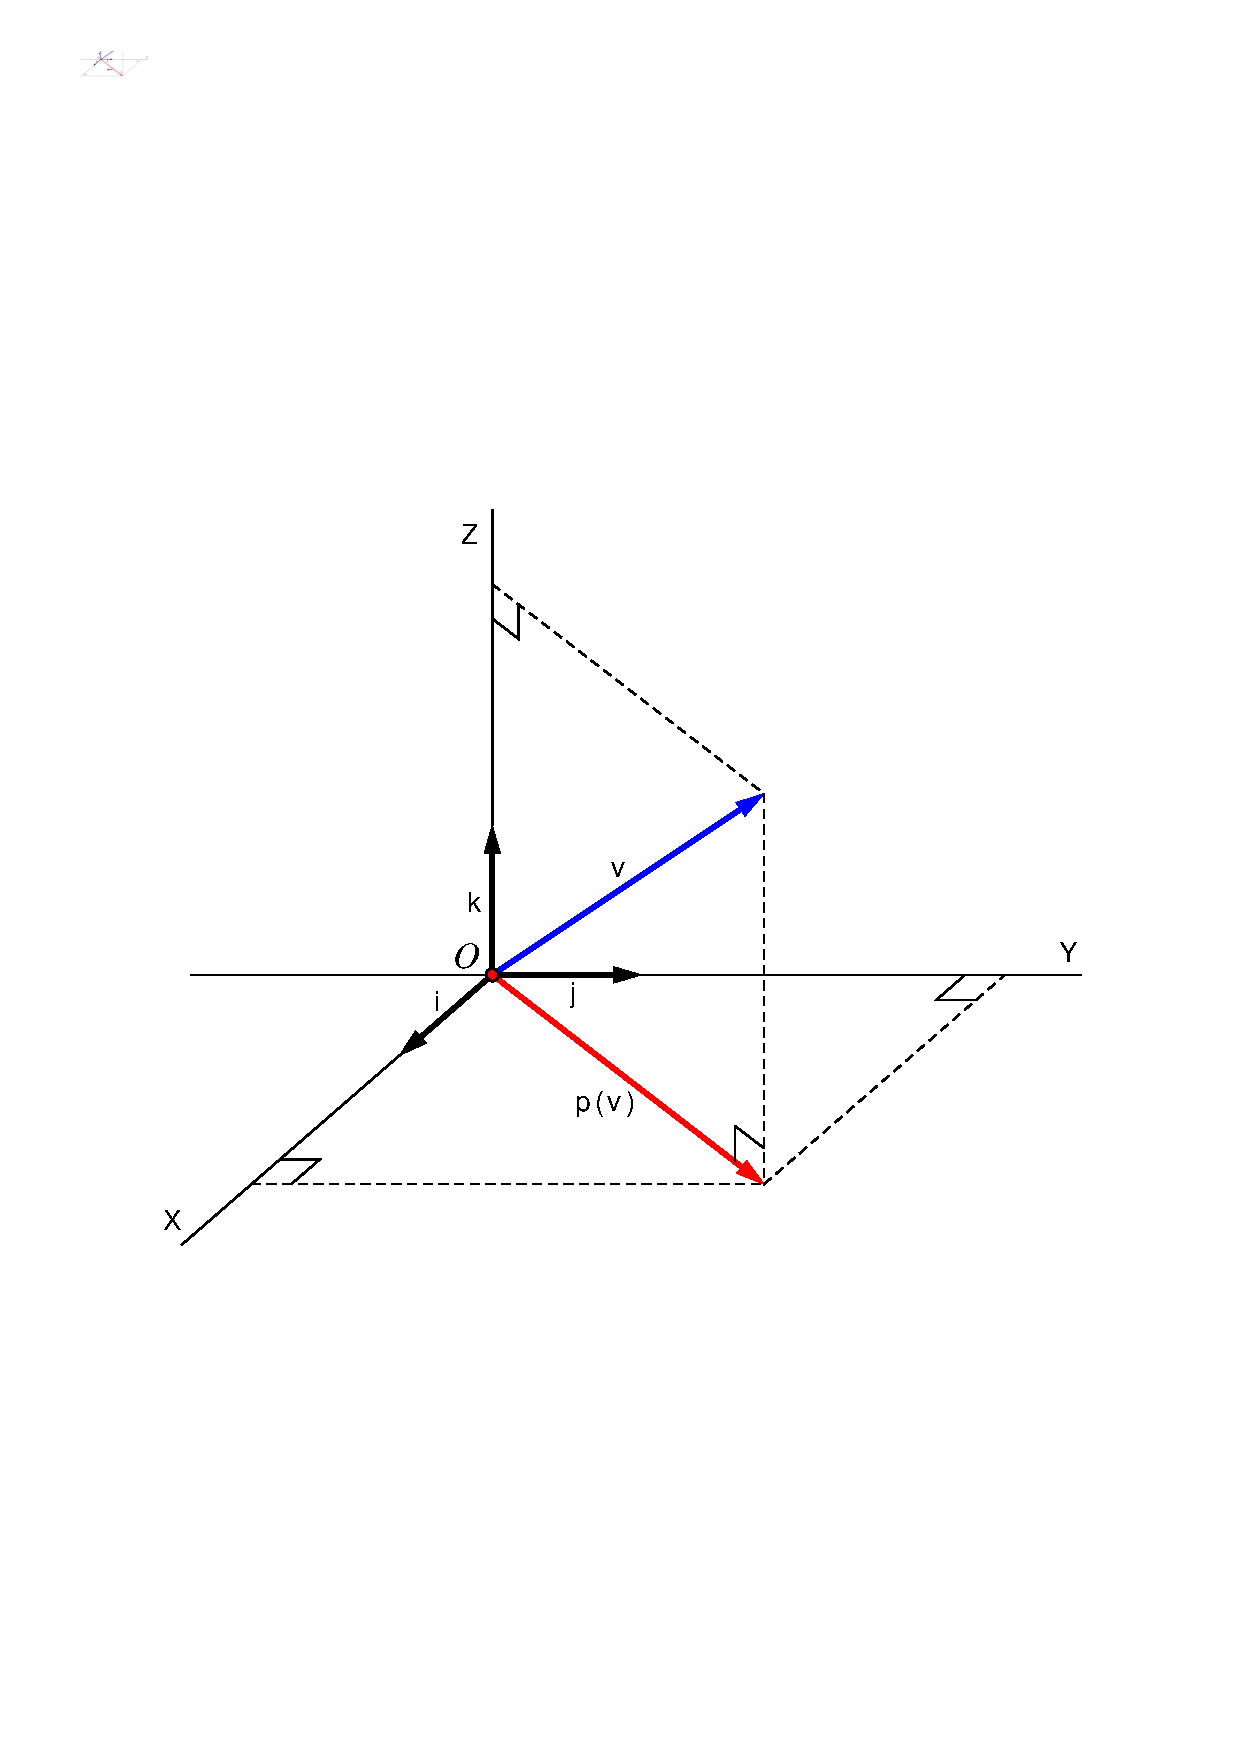
\includegraphics[trim=2cm 8cm 2cm
 8cm,width=0.50\textwidth,clip]{projektion.pdf}
  \\Figur 8.12: Projektion ned i  $(X,Y)$-planen
\end{center}

Vis at $\,p\,$ er lineær, og opstil afbildningsmatricen $\matind ePe$ for $p$. Bestem en basis for projektionens kerne og billedrum. Tjek at dimensionssætningen er opfyldt.

\end{exercise}
%\begin{example}
%Når man fotograferer, afbildes rummet på en plan, objektet mister en dimension ved afbildningen. Inspiration.\\TO BE DONE.
%\end{example}
%\begin{theorem}[]\label{tn8.struktur3}
%Finde afbildningen ud fra billederne af $n$ lineært uafhængige %vektorer. \\
%TO BE DONE.
%\end{theorem}

%\begin{exercise}
%Linealer afbildes på linealer. En lineær afbildning er bestemt ved %to foreliggende linealer.\\
%TO BE DONE.
%Figur 8.11. TO BE DONE
%\end{exercise}


\section{Ændring af afbildningsmatricen når der skiftes basis}\label{tn8.AfsnitBasisskifte}

Afbildningsmatricen for en lineær afbildning $\,f:V\rightarrow W\,$ kan kun opstilles når der er valgt en basis i $V$ og en basis i $W$. Med afbildningsmatricens symbol $\,\matind cFa$ viser vi netop at dens grundlag er  en given basis $a$ i $V$ og en given basis $c$ i $W$.\bs
Ofte ønsker man at skifte basen i $V$ eller basen i $W$. I det første tilfældes ændres koordinaterne for de vektorer $\mathbf x\in V$ der skal afbildes, mens koordinaterne for deres billeder $\mathbf y = f(\mathbf x)$ er uforandrede. I det andet tilfælde er omvendt. Her er koordinaterne for $\mathbf x$ er de samme, mens billedets koordinaterne skifter. Hvis der skiftes basis i både i $V$ og $W$, så ændres koordinaterne både for $\mathbf x$ og $\mathbf y =f(\mathbf x)$.\bs
I dette afsnit opstilles metoder til at finde den nye  afbildningsmatrix for $f\,$, når der skiftes basis i enten definitionsrummet, dispositionsrummet eller i dem begge. Først viser vi hvordan en vektors koordinater skifter, når der skiftes basis i vektorrummet (som nærmere beskrevet i \tref{NUID18-tn7.methSkifte}{metode} i eNote 7.)\bs
Antag at der er i $V$ er givet en $a$-basis $(\ma_1,\ma_2,\ldots,\ma_n)\,$, og at der vælges en ny $b$-basis $(\mb_1,\mb_2,\ldots,\mb_n)\,$ i $V$. Hvis en vektor $\mathbf x$ har $\,b$-koordinatvektoren $\,\vekind bx\,$, så kan dens $\,a$-koordinatvektor udregnes ved matrixvektor-produktet 
\begin{equation}\label{tn8.skiftAfbM1}
\vekind av = \matind aMb\,\vekind bv\,
\end{equation}
hvor \textit{basisskiftematricen} $\,\matind aMb\,$ er givet ved
\begin{equation}\label{tn8.skiftAfbM2}
\matind aMb=\begin{matr}{rrrr}\vekind ab_1&\vekind ab_2&\ldots&\vekind ab_n\end{matr}\,.
\end{equation}
Vi viser nu to eksempler på brug af (\ref{tn8.skiftAfbM2}). I det første er det de ``nye'' koordinater der er givne hvorefter de ``gamle'' beregnes. I det andet er det omvendt: de ``gamle'' kendes, og de ``nye'' bestemmes.

\begin{example}[Fra nye koordinater til gamle]\label{tn8.exAbildM1}
I et 3-dimensionalt vektorrum $V$ er der givet en basis $(\ma_1,\ma_2,\ma_3)\,$, hvorefter der vælges en ny basis bestående af vektorerne $$\mb_1=\ma_1-\ma_3,\, \mb_2=2\ma_1-2\ma_2+\ma_3\,\,\,\mathrm{og}\,\,\,\mb_3=-3\ma_1+3\ma_2-\ma_3\,.$$
\textit{Opgave}: Bestem koordinatvektoren $\,\vekind ax\,$ for $\,\mathbf x=\mb_1+2\mb_2+3\mb_3\,$.\bs
\textit{Løsning}: Først ser vi at
\begin{equation}\label{tn8.exAbildM1.1}
\vekind bx = \begin{matr}{r}1\\2\\3\end{matr}\mathrm{\;\;og\;\;}
\matind aMb=\begin{matr}{rrr}1&2&-3\\0&-2&3\\-1&1&-1\end{matr}\,.
\end{equation}
Herefter får vi
\begin{equation}\label{tn8.exAbildM1.2}
\vekind ax =\matind aMb \,\vekind bx=
\begin{matr}{rrr}1&2&-3\\0&-2&3\\-1&1&-1\end{matr}\,
\begin{matr}{r}1\\2\\3\end{matr}=
\begin{matr}{r}-4\\5\\-2\end{matr}\,.
\end{equation}
\end{example}

\begin{example}[Fra gamle koordinater til nye]\label{tn8.exAbildM2}
I et 2-dimensionalt vektorrum $W$ er der givet en basis $(\mc_1,\mc_2)\,$, hvorefter der vælges en ny basis bestående af vektorerne $$\md_1=2\mc_1+\mc_2\,\,\,\mathrm{og}\,\,\,\md_2=\mc_1+\mc_2\,.$$
\textit{Opgave}: Bestem koordinatvektoren $\,\vekind dy\,$ for $\,\mathbf y=10\mc_1+6\mc_2\,$.\bs
\textit{Løsning}: Først ser vi at
\begin{equation}\label{tn8.exAbildM2.1}
\vekind cy = \begin{matr}{r}10\\6\end{matr}\mathrm{\;\;og\;\;}
\matind cMd=\begin{matr}{rr}2&1\\1&1\end{matr}\,
\Rightarrow
\matind dMc=(\matind cMd)^{\mathrm{-}1}=\begin{matr}{rr}1&-1\\-1&2\end{matr}\,.
\end{equation}
\begin{equation}\label{tn8.exAbildM2.2}
\vekind dy =\matind dMc \,\vekind cy = 
\begin{matr}{rr}1&-1\\-1&2\end{matr}\,  
\begin{matr}{r}10\\6\end{matr}=\begin{matr}{r}4\\2\end{matr}\,.
\end{equation}
%Vi tilføjer at $\,\mathbf y=-2\md_1+5\md_2\,$.\\
\end{example}

\subsection{Basisskifte i definitionsrummet}

\begin{center}
		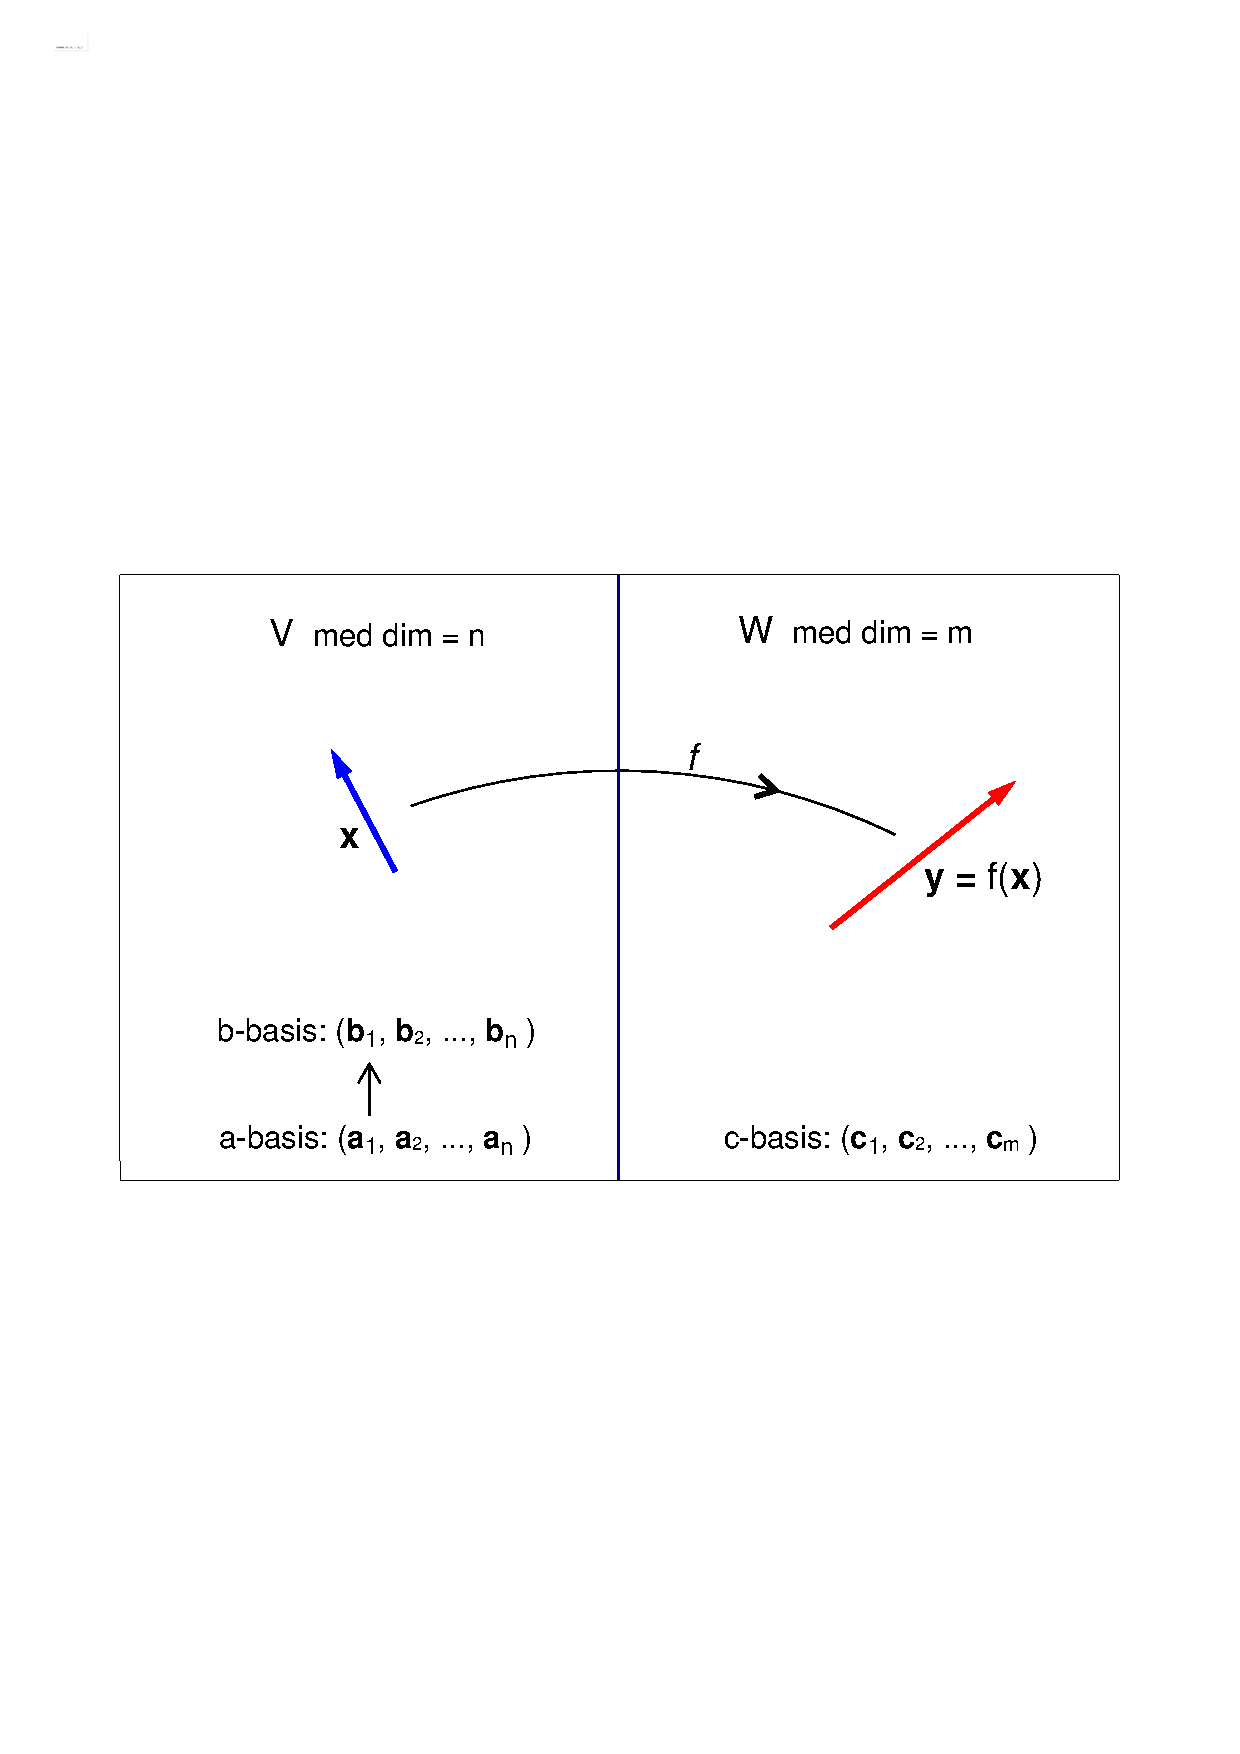
\includegraphics[trim=2cm 9cm 2cm
 9cm,width=0.60\textwidth,clip]{linAfbVW2.pdf}
  \\Figur 8.12: Lineær afbildning 
\end{center}

På figur 8.12 er der givet en lineær afbildning $\,f:V\rightarrow W\,$ som med hensyn til $a$-basis i $V$ og $c$-basis i $W$ har en afbildningsmatrix $\,\matind cFa\,$. Vi skifter basis i $V$ fra $a$-basis til $b$-basis. Afbildningsmatricen for $f$ har nu symbolet $\,\matind cFb\,$. Lad os finde den. Ligningen
$$
\mathbf y = f(\mathbf x)$$
oversættes til koordinater og omformes:
$$
\vekind cy =\matind cFa\,\vekind ax
=\matind cFa\,(\matind aMb\,\vekind bx)
=(\matind cFa\,\matind aMb)\,\vekind bx \,.
$$
Heraf kan vi udlede at afbildningsmatricen for $f$ med hensyn til $b$-basis i $V$ og $c$-basis i $W$ dannes ved et matrixprodukt:
\begin{equation}%\label{tn8.bFa}
 \matind cFb=\matind cFa\,\matind aMb\,.
\end{equation}

\begin{example}[Ændring af afbildningsmatrix]%\label{tn8.exAbildM3}
Vi betrager det 3-dimensionale vektorrum $V$ som er behandlet i eksempel \ref{tn8.exAbildM1}, og det 2-dimensionale vektorrum $W$ som er behandlet i eksempel \ref{tn8.exAbildM2}. En lineær afbildning $\,f:V\rightarrow W\,$ er givet ved afbildningsmatricen:
$$
\matind cFa=\begin{matr}{rrr}9&12&7\\6&8&5\end{matr}\,.
$$
\textit{Opgave}: Bestem $\mathbf y=f(\mathbf x)$ hvor $\mathbf x=\mb_1+2\mb_2+3\mb_3\,$.\bs
\textit{Løsning}: Vi afprøver to forskellige veje.
1) Vi bruger $a$-koordinaterne $\mathbf x$ som fundet i (\ref{tn8.exAbildM1.1}):
$$\vekind cy=\matind cFa\,\vekind ax=
\begin{matr}{rrr}9&12&7\\6&8&5\end{matr}\,\begin{matr}{r}-4\\5\\-2\end{matr}
=\begin{matr}{r}10\\6\end{matr}\,.$$
2) Vi ændrer afbildningsmatricen for $f\,$:
$$
\matind cFb=\matind cFa\,\matind aMb =
\begin{matr}{rrr}9&12&7\\6&8&5\end{matr}\,
\begin{matr}{rrr}1&2&-3\\0&-2&3\\-1&1&-1\end{matr}
=\begin{matr}{rrr}2&1&2\\1&1&1\end{matr}\,.
$$
Så kan vi direkte bruge de givne $b$-koordinater for $\mathbf x\,$:
$$\vekind cy=\matind cFb\,\vekind bx=
\begin{matr}{rrr}2&1&2\\1&1&1\end{matr}\,\begin{matr}{r}1\\2\\3\end{matr}
=\begin{matr}{r}10\\6\end{matr}\,.$$
I begge tilfælde får vi $\mathbf y = 10\mc_1+6\mc_2\,$.
 
\end{example}
\subsection{Basisskifte i dispositionsrummet}

\begin{center}
		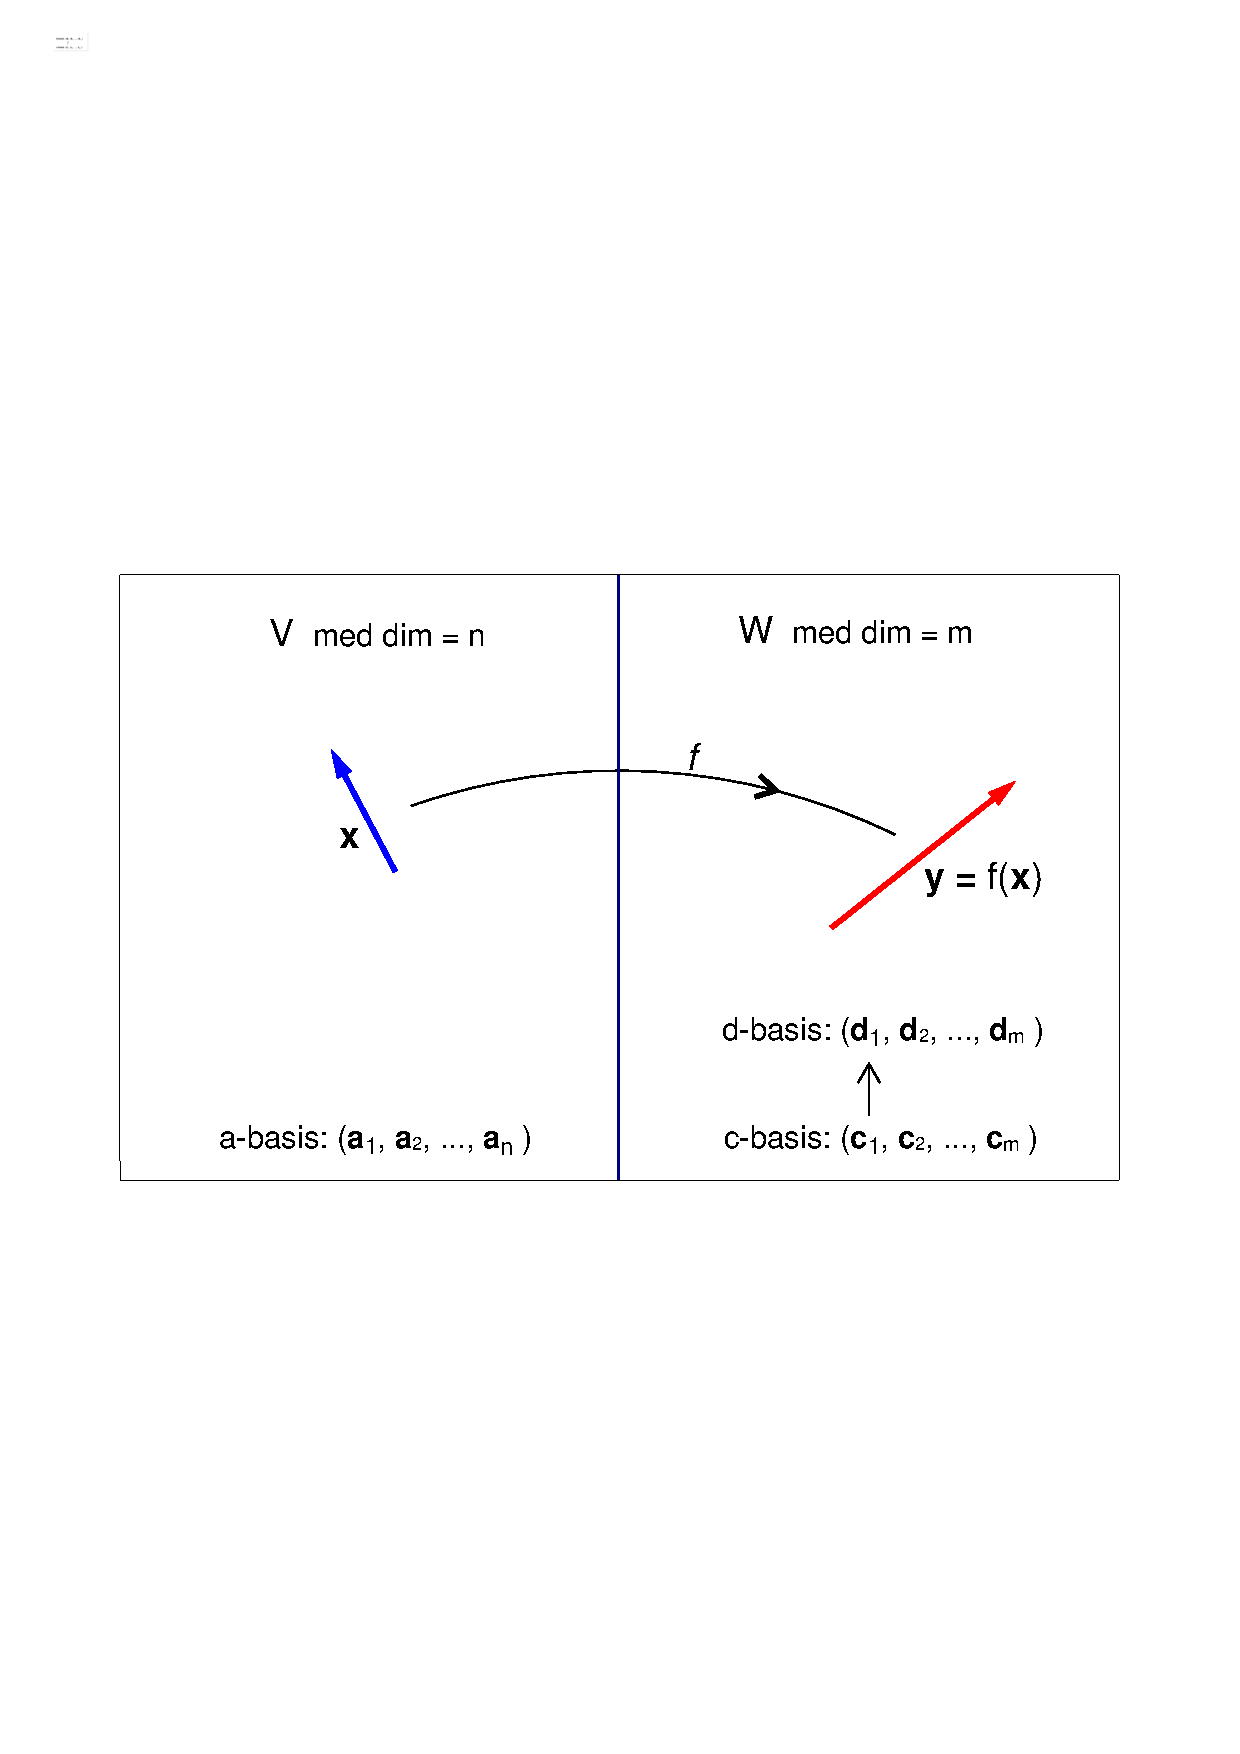
\includegraphics[trim=2cm 9cm 2cm
 9cm,width=0.60\textwidth,clip]{linAfbVW3.pdf}
  \\Figur 8.13: Lineær afbildning 
\end{center}

På figur 8.13 er der givet en lineær afbildning $\,f:V\rightarrow W\,$ som med hensyn til $a$-basis i $V$ og $c$-basis i $W$ har en afbildningsmatrix $\,\matind cFa\,$. Vi skifter basis i $W$ fra $c$-basis til $d$-basis. Afbildningsmatricen for $f$ har nu symbolet $\,\matind dFa\,$. Lad os finde den. Ligningen $$ \mathbf y = f(\mathbf x)$$ oversættes til matrixligningen $$
\vekind cy =\matind cFa\,\vekind ax $$
som er ensbetydende med
$$
\matind dMc\,\vekind cy=\matind dMc\,(\matind cFa\,\vekind ax)$$
hvoraf fås
$$
\vekind dy=(\matind dMc\,\matind cFa)\,\vekind ax\,.
$$ 

Heraf udleder vi at afbildningsmatricen for $f$ med hensyn til $a$-basis i $V$ og $d$-basis i $W$ dannes ved et matrixprodukt:
\begin{equation}%\label{tn8.bFa}
 \matind dFa=\matind dMc\,\matind cFa\,.
\end{equation}

\begin{example}[Ændring af afbildningsmatrix]%\label{tn8.exAbildM3}
Vi betrager det 3-dimensionale vektorrum $V$ som er behandlet i eksempel \ref{tn8.exAbildM1}, og det 2-dimensionale vektorrum $W$ som er behandlet i eksempel \ref{tn8.exAbildM2}. En lineær afbildning $\,f:V\rightarrow W\,$ er givet ved afbildningsmatricen:
$$
\matind cFa=\begin{matr}{rrr}9&12&7\\6&8&5\end{matr}\,.
$$
\textit{Opgave}: Givet vektoren $\,\mathbf x=-4\ma_1+5\ma_2-2\ma_3\,$. Bestem billedet $\mathbf y=f(\mathbf x)$ som en linearkombination af $\mathbf d_1$ og $\mathbf d_2\,$. \bs
\textit{Løsning}: Vi afprøver to forskellige veje.\\
1) Vi bruger den givne afbildningsmatrix:
$$\vekind cy=\matind cFa\,\vekind ax=
\begin{matr}{rrr}9&12&7\\6&8&5\end{matr}\,\begin{matr}{r}-4\\5\\-2\end{matr}
=\begin{matr}{r}10\\6\end{matr}\,.$$
Og oversætter resultatet til $d$-koordinater ved hjælp af (\ref{tn8.exAbildM2.2}):
$$\vekind dy=\matind dMc\,\vekind cy = 
\begin{matr}{rr}1&-1\\-1&2\end{matr} \begin{matr}{r}10\\6\end{matr}
=\begin{matr}{r}4\\2\end{matr}\,$$
2) Vi ændrer afbildningsmatricen for $f$ ved hjælp af (\ref{tn8.exAbildM2.1}):
$$
\matind dFa=\matind dMc\matind cFa\, =
\begin{matr}{rr}1&-1\\-1&2\end{matr}\,
\begin{matr}{rrr}9&12&7\\6&8&5\end{matr}\,
=\begin{matr}{rrr}3&4&2\\3&4&3\end{matr}\,.
$$
Så kan vi direkte aflæse $d$-koordinaterne:
$$\vekind dy=\matind dFa\,\vekind ax=
\begin{matr}{rrr}3&4&2\\3&4&3\end{matr}\,\begin{matr}{r}-4\\5\\-2\end{matr}
=\begin{matr}{r}4\\2\end{matr}\,.$$
I begge tilfælde får vi $\mathbf y = 4\md_1+2\md_2\,$.
\end{example}

\subsection{Basisskifte i både definitions- og dispositionsrummet}
\begin{center}
		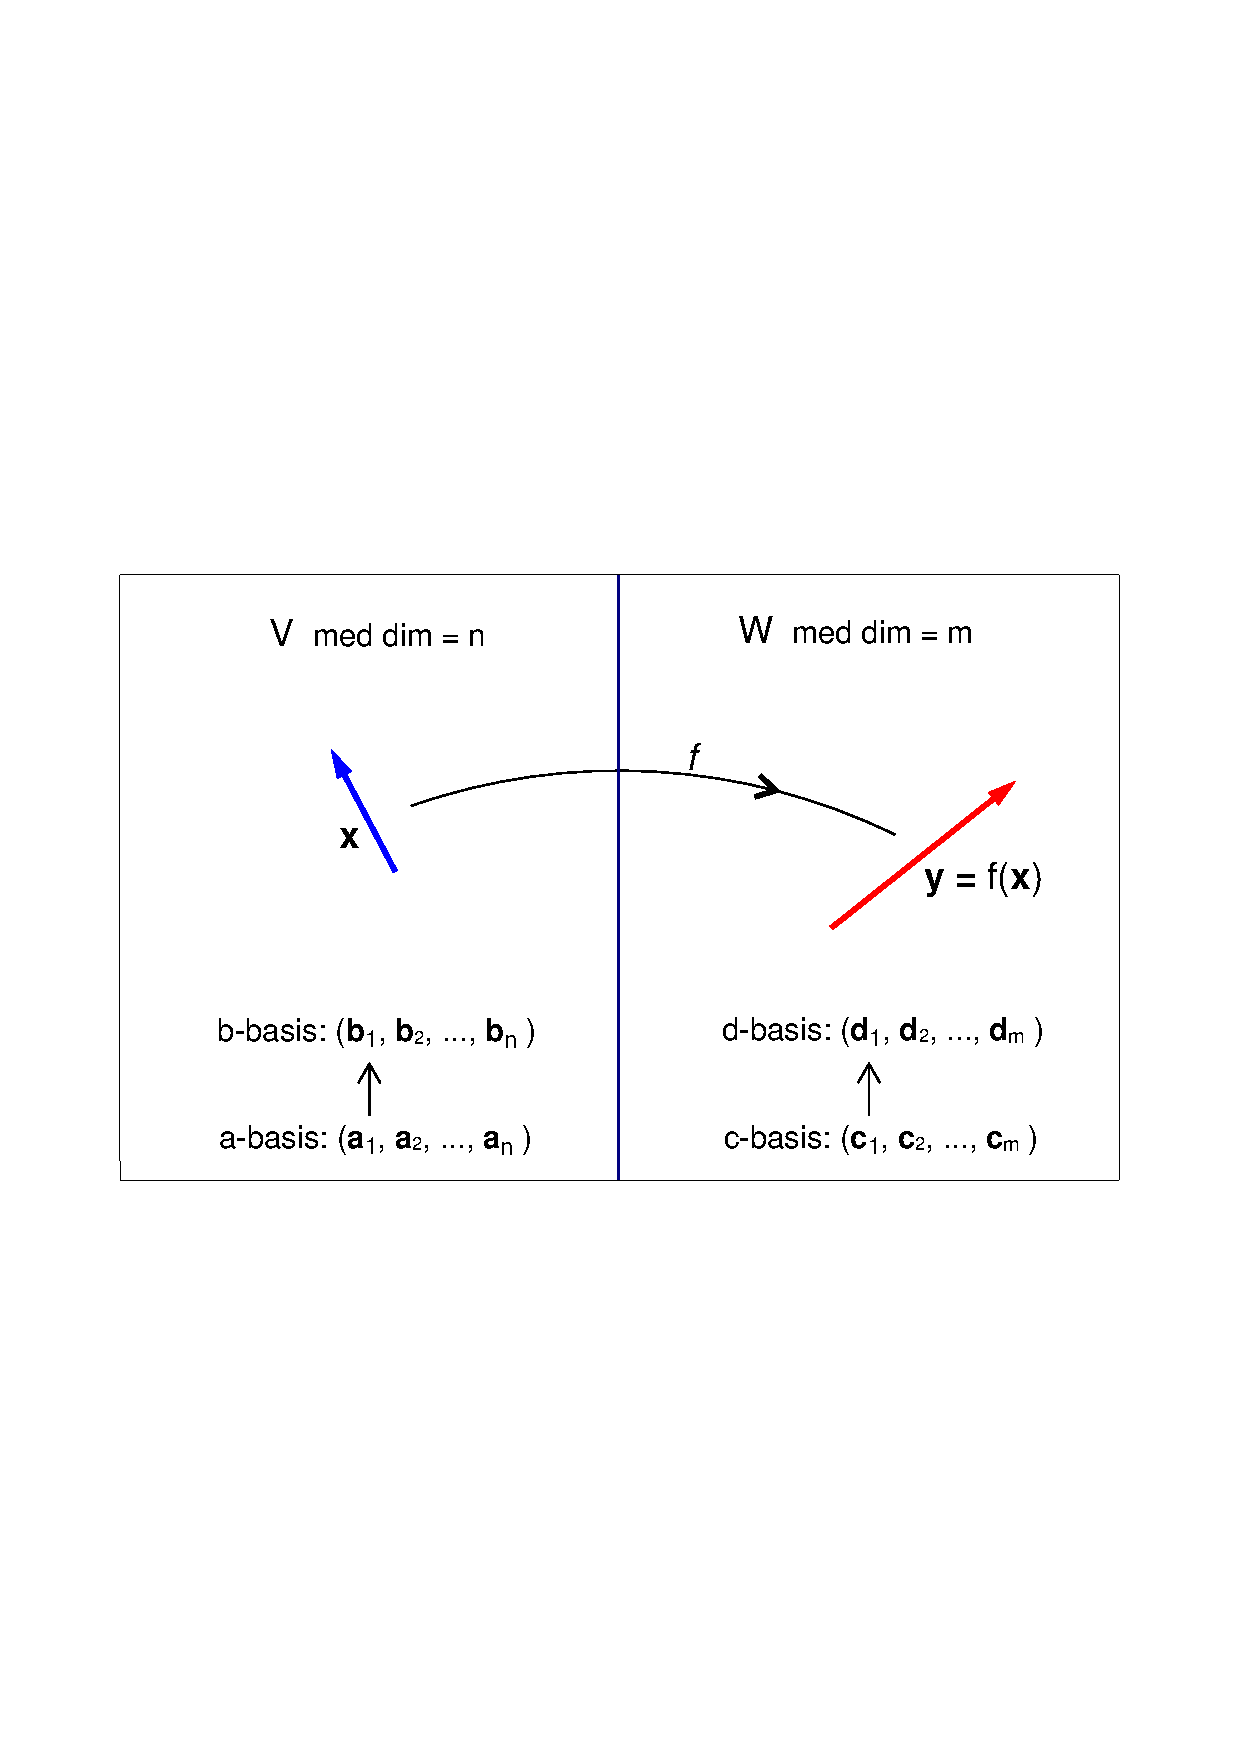
\includegraphics[trim=2cm 9cm 2cm
 9cm,width=0.60\textwidth,clip]{linAfbVW4.pdf}
  \\Figur 8.14: Lineær afbildning 
\end{center}

På figur 8.14 er der er givet en lineær afbildning $\,f:V\rightarrow W\,$ som med hensyn til $a$-basis i $V$ og $c$-basis i $W$ har afbildningsmatricen $\,\matind cFa\,$. Vi skifter basis i $V$ fra $a$-basis til $b$-basis, og i $W$ fra $c$-basis til $d$-basis. Afbildningsmatricen for $f$ har nu symbolet $\,\matind dFb\,$.Lad os finde den. Ligningen 
$$
y = f(\mathbf x)$$ svarer i koordinater til
$$\vekind cy=\matind cFa\,\vekind ax $$
som er ensbetydende med
$$\matind dMc\,\vekind cy=\matind dMc\,\big(\,\matind cFa\,(\matind aMb\,\vekind bx)\,\big)$$ hvoraf fås
$$\vekind dy=(\matind dMc\,\matind cFa\,\matind aMb)\,\vekind bx\,.$$

Heraf udleder vi at afbildningsmatricen for $f$ med hensyn til $b$-basis i $V$ og $d$-basis i $W$ dannes ved et matrixprodukt:
\begin{equation}\label{tn8.bFa}
 \matind dFb=\matind dMc\,\matind cFa\,\matind aMb\,.
\end{equation}
\begin{example}[Ændring af afbildningsmatrix]%\label{tn8.exAbildM3}
Vi betrager det 3-dimensionale vektorrum $V$ som er behandlet i eksempel \ref{tn8.exAbildM1}, og det 2-dimensionale vektorrum $W$ som er behandlet i eksempel \ref{tn8.exAbildM2}. En lineær afbildning $\,f:V\rightarrow W\,$ er givet ved afbildningsmatricen:
$$
\matind cFa=\begin{matr}{rrr}9&12&7\\6&8&5\end{matr}\,.
$$
\textit{Opgave}: Givet vektoren $\,\mathbf x=\mb_1+2\mb_2+3\mb_3\,$. Bestem $\mathbf y=f(\mathbf x)$ som en linearkombination af $\mathbf d_1$ og $\mathbf d_2\,$.\bs
\textit{Løsning}: Vi ændrer afbildningsmatricen ved hjælp af (\ref{tn8.exAbildM2.1}) og (\ref{tn8.exAbildM1.1}):
$$
\matind dFb=\matind dMc\,\matind cFa\,\matind aMb =
\begin{matr}{rr}1&-1\\-1&2\end{matr}\,
\begin{matr}{rrr}9&12&7\\6&8&5\end{matr}\,
\begin{matr}{rrr}1&2&-3\\0&-2&3\\-1&1&-1\end{matr}
=\begin{matr}{rrr}1&0&1\\0&1&0\end{matr}\,.
$$
Så kan vi direkte bruge de givne $b$-koordinater og direkte aflæse $d$-koordinaterne:
$$\vekind dy=\matind dFb\,\vekind bx=
\begin{matr}{rrr}1&0&1\\0&1&0\end{matr}\,\begin{matr}{r}1\\2\\3\end{matr}
=\begin{matr}{r}4\\2\end{matr}\,.$$
Konklusion: $\mathbf y = 4\md_1+2\md_2\,$.\bs
Basisskiftet viser sig at være ganske praktisk. Med den nye afbildningsmatrix $\,\matind dFb\,$ er det meget nemmere at udregne billedvektorer: man lægger blot første- og tredjekoordinaten fra den givne vektor sammen og beholder andenkoordinaten!  
\end{example}

\subsection{Opsummering vedrørende basisskifte}

Vi samler resultaterne vedrørende basisskifte i de foregående underafsnit i den følgende metode:

\begin{method}[Ændring af afbildningsmatrix ved basisskifte]
I vektorrummet $V$ er der givet en basis $\,(\ma_1,\ma_2,\ldots,\ma_n)\,$ og en ny basis $\,(\mb_1,\mb_2,\ldots,\mb_n)\,$. I vektorrummet $W$ er der givet en basis $\,(\mc_1,\mc_2,\ldots,\mc_m)\,$ og en ny basis $\,(\md_1,\md_2,\ldots,\md_m)\,$.\bs
Hvis $f$ er en lineær afbildning $\,f:V\rightarrow W\,$ som med hensyn til $a$-basis i $V$ og $c$-basis i $W$ har afbildningsmatricen $\matind cFa\,$, så gælder:
\begin{enumerate}
\item
Afbildningsmatricen for $\,f\,$ med hensyn til $b$-basis i $V$ og $c$-basis i $W$ er
\begin{equation}\label{tn8.methSkiftAfbildM1}
\matind cFb=\matind cFa\,\matind aMb\,.\end{equation}
\item
Afbildningsmatricen for $\,f\,$ med hensyn til $a$-basis i $V$ og $d$-basis i $W$ er
\begin{equation}\label{tn8.methSkiftAfbildM2}
\matind dFa=(\matind cMd)^{\mathrm{-}1}\,\matind cFa\, = \matind dMc \, \matind cFa\,.\end{equation}
\item
Afbildningsmatricen for $\,f:\,$ med hensyn til $b$-basis i $V$ og $d$-basis i $W$ er 
\begin{equation}\label{tn8.methSkiftAfbildM3}
\matind dFb=(\matind cMd)^{\mathrm{-}1}\,\matind cFa\,\matind aMb\, = \matind dMc \, \matind cFa \, \matind aMb \,.\end{equation}
\end{enumerate}
I de tre formler har vi brugt basisskiftematricerne:
$$\matind aMb=
\begin{matr}{rrrr}\vekind ab_1 & \vekind ab_2 & \cdots & \vekind ab_n \end{matr}\;\;\mathrm{og}\;\;\matind cMd=
\begin{matr}{rrrr}\vekind cd_1 & \vekind cd_2 & \cdots & \vekind cd_m \end{matr}\,.$$
\end{method}


%%%%%%%%%%%%%%%%%%%%%%%%%%%%%%%%%%%%%%%
%%% HER SKAL DU STOPPE MED AT SKRIVE %%%%%%%%
%%%%%%%%%%%%%%%%%%%%%%%%%%%%%%%%%%%%%%%%%%%%%
%%%%%%%%%%%%%%%%%%%%%%%%%%%%%%%%%%%%%%%%%%%%%


\end{document} 